\documentclass[mathpazo]{cicp}

\usepackage{times,amsmath,amsbsy,amssymb,amscd,mathrsfs}
%\usepackage{slashbox}\usepackage{graphicx,subfigure,epstopdf,wrapfig,chemarrow}

\usepackage{algorithm2e} 
\usepackage{multicol,multirow}
\usepackage{mathtools}
\usepackage[usenames,dvipsnames,svgnames,table]{xcolor}
\usepackage[all]{xy}
\usepackage{wrapfig}
\usepackage{tcolorbox}
\usepackage{booktabs} 

\usepackage[labelformat=empty]{subfig}
%\usepackage[hang,small,bf]{caption}

\usepackage{tikz,tikz-cd}
\usepackage[utf8]{inputenc}
\usepackage{pgfplots} 
\usepackage{pgfgantt}
\usepackage{pdflscape}
\pgfplotsset{compat=newest} 
\pgfplotsset{plot coordinates/math parser=false}
\newlength\fwidth

%\usepackage[notcite,notref]{showkeys}
\usepackage[numbered]{mcode}

\definecolor{myBlue}{rgb}{0.0,0.0,0.55}
%\definecolor{green}{rgb}{0.0,0.7,0.2}
\usepackage[pdftex,colorlinks=true,citecolor=myBlue,linkcolor=myBlue]{hyperref}

\usepackage[hyperpageref]{backref}

%\newcommand{\LC}[1]{\textcolor{cyan}{#1}}
\newcommand{\LC}[1]{\textcolor{red!80!black}{#1}}
\newcommand{\XH}[1]{\textcolor{cyan}{#1}}
\newcommand{\CC}[1]{\textcolor{orange}{#1}}

\usepackage{comment,enumerate,multicol,xspace}

  \newcounter{mnote}
  \setcounter{mnote}{0}
  \newcommand{\mnote}[1]{\addtocounter{mnote}{1}
    \ensuremath{{}^{\bullet\arabic{mnote}}}
    \marginpar{\footnotesize\em\color{red}\ensuremath{\bullet\arabic{mnote}}#1}}
  \let\oldmarginpar\marginpar
    \renewcommand\marginpar[1]{\-\oldmarginpar[\raggedleft\footnotesize #1]%
    {\raggedright\footnotesize #1}}

%\usepackage[pdftex,dvipsnames]{xcolor}

%\usepackage{xargs} % Use more than one optional parameter in a new commands
%\usepackage[colorinlistoftodos,prependcaption,textsize=footnotesize]{todonotes}
%
%\newcounter{mycomment}
%\newcommand{\mycomment}[2][]{%
%% initials of the author (optional) + note in the margin
%\refstepcounter{mycomment}%
%{%
%\todo[linecolor=blue,backgroundcolor=blue!25,bordercolor=blue]{%
%\textbf{Comment [{\sc #1\themycomment}]:}\\#2}%
%}}
%
%\newcommandx{\change}[2][1=]
%{\todo[linecolor=OliveGreen,backgroundcolor=OliveGreen!25,bordercolor=OliveGreen,#1]{%
%{\sc Change}:\\#2}}
%
%\newcommandx{\improvement}[2][1=]
%{\todo[linecolor=Plum,backgroundcolor=Plum!25,bordercolor=Plum,#1]{%
%{\sc Improvement}:\\#2}}
%
%\newcommandx{\unsure}[2][1=]
%{\todo[linecolor=red,backgroundcolor=red!25,bordercolor=red,#1]{%
%{\sc Unsure}:\\ #2}}
%

% \newcommand{\mnote}[1]{}
\newcommand{\breakline}{
\begin{center}
------------------------------------------------------------------------------------------------------------
\end{center}
}
%\usepackage{geometry}
%%\usepackage{graphicx,pst-eps,epstopdf}
%\geometry{letterpaper, margin=1.5in}

%\newtheorem{theorem}{Theorem}[section]
%\newtheorem{lemma}[theorem]{Lemma}
\newtheorem{corollary}[theorem]{Corollary}
%\newtheorem{proposition}[theorem]{Proposition}
%\newtheorem{definition}[theorem]{Definition}
%\newtheorem{example}[theorem]{Example}
\newtheorem{exercise}[theorem]{Exercise}
\newtheorem{question}[theorem]{Question}
%\newtheorem{remark}[theorem]{Remark}
\newtheorem{alg}[theorem]{Algorithm}
%\newtheorem{answer}[proof]{Question}

\newcommand{\dx}{\,{\rm d}x}
\newcommand{\dd}{\,{\rm d}}
\newcommand{\deq}{\stackrel{\rm def}{=}}
\newcommand{\mbb}{\mathbb}
\newcommand{\mbf}{\bs}
\newcommand{\bs}{\boldsymbol}
\newcommand{\mcal}{\mathcal}
\newcommand{\mc}{\mcode}
\newcommand{\lla}{\langle}
\newcommand{\rra}{\rangle}
\newcommand{\supp}{\operatorname{supp}}
\newcommand{\range}{\operatorname{range}}
\newcommand{\PartSize}{\fontsize{0.85cm}{0.85cm}\selectfont} 
\newcommand{\mscr}{\mathscr}
\DeclarePairedDelimiter\ceil{\lceil}{\rceil}
\DeclarePairedDelimiter\floor{\lfloor}{\rfloor}

%\newcommand{\span}{\rm span}
\newcommand{\red}{\color{red}}
\newcommand{\green}{\color{green}}
\newcommand{\blue}{\color{blue}}
\newcommand{\gray}{\color{gray}}

%\DeclareMathOperator*{\curl}{curl}
\DeclareMathOperator*{\img}{img}
\DeclareMathOperator*{\spa}{span}
\DeclareMathOperator*{\diag}{diag}
\newcommand{\curl}{{\rm curl\,}}
\renewcommand{\div}{\operatorname{div}}
%\renewcommand{\grad}{\operatorname{grad}}
\newcommand{\grad}{{\rm grad\,}}
%\DeclareMathOperator*{\tr}{tr}
\DeclareMathOperator*{\rot}{rot}
\DeclareMathOperator*{\var}{Var}
\DeclareMathOperator{\rank}{rank}
\DeclareMathOperator{\dist}{dist}
%\DeclareMathOperator{\span}{span}
\newcommand{\tr}{\operatorname{tr}}
\newcommand{\dev}{\operatorname{dev}}
\newcommand{\sym}{\operatorname{sym}}
\newcommand{\skw}{\operatorname{skw}}
\newcommand{\spn}{\operatorname{spn}}
\newcommand{\mspn}{\operatorname{mspn}}
\newcommand{\vspn}{\operatorname{vspn}}
\newcommand{\mskw}{\operatorname{mskw}}
\newcommand{\vskw}{\operatorname{vskw}}
\newcommand{\defm}{\operatorname{def}}
\newcommand{\hess}{\operatorname{hess}}
\newcommand{\inc}{\operatorname{inc}}
\newcommand{\dex}{\operatorname{dex}}

\newcommand{\step}[1]{\noindent\raisebox{1.5pt}[10pt][0pt]{\tiny\framebox{$#1$}}\xspace}

%\usepackage[margins]{trackchanges}
%\renewcommand{\initialsOne}{chen}

\newcommand{\norm}[1]{\left\Vert#1\right\Vert}
\newcommand{\snorm}[1]{\left\vert#1\right\vert}
\newcommand{\vertiii}[1]{{\left\vert\kern-0.25ex\left\vert\kern-0.25ex\left\vert #1 
    \right\vert\kern-0.25ex\right\vert\kern-0.25ex\right\vert}}


\let\listofalgorithms\relax
\let\listalgorithmname\relax
\usepackage{algorithm}
\usepackage{algpseudocode}
\usepackage{stmaryrd}
\usepackage{scalefnt}
\usepackage{graphicx}
\usepackage{caption}
\usepackage{listings}
\usepackage[T1]{fontenc}
\usepackage{siunitx}
\usepackage{float}

\definecolor{codegray}{rgb}{0.95,0.95,0.95}
\definecolor{codeframe}{rgb}{0.5,0.5,0.5}
\definecolor{codecomment}{rgb}{0.4,0.4,0.4}
\definecolor{codegreen}{rgb}{0,0.6,0}
\definecolor{codeblue}{rgb}{0,0,0.8}
\definecolor{codepurple}{rgb}{0.6,0,0.6}

\lstset{
	backgroundcolor=\color{codegray},    % 浅灰色背景
	basicstyle=\ttfamily\scriptsize,     % 使用更小的等宽字体
	breakatwhitespace=false,
	breaklines=true,
	captionpos=t,                        % 标题位置在 top
	commentstyle=\color{codecomment},    % 注释样式
	frame=lines,                         % 只在上下添加边框线
	rulecolor=\color{codeframe},         % 边框颜色
	keywordstyle=\color{codepurple},     % 关键字样式
	numbersep=5pt,                       % 行号和代码的距离
	numberstyle=\tiny\color{codecomment},% 行号的样式
	showspaces=false,                    % 不显示空格符号
	showstringspaces=false,              % 不显示字符串中的空格符号
	showtabs=false,                      % 不显示制表符
	stringstyle=\color{codegreen},       % 字符串样式
	tabsize=4,                           % 制表符等于4个空格
	numbers=left,                        % 在左侧显示行号
	xleftmargin=2em,                     % 左边距,为行号腾出空间
	framexleftmargin=1.5em,              % 框架左边距
	aboveskip=10pt,                      % 上边距
	belowskip=10pt,                      % 下边距
	keepspaces=true                     % 保持用户输入的空格
}

\newcommand{\Oplus}{\ensuremath{\vcenter{\hbox{\scalebox{1.5}{$\oplus$}}}}}
\newcommand{\prox}{\operatorname{Prox}}

\renewcommand{\lstlistingname}{Code}
\renewcommand{\thealgorithm}{2.\arabic{algorithm}}

\lstset{basicstyle=\ttfamily}
\captionsetup[figure]{font=rm}

%%%%% author macros %%%%%%%%%
% place your own macros HERE
%%%%% end %%%%%%%%%

\begin{document}
\title[Efficient Multi-Backend Implementation]{SOPTX: A High-Performance Multi-Backend Framework for Topology Optimization}

%%%%% author(s) :
% single author:
% \author[name in running head]{AUTHOR\corrauth}
% [name in running head] is NOT OPTIONAL, it is a MUST.
% Use \corrauth to indicate the corresponding author.
% Use \email to provide email address of author.
% \footnote and \thanks are not used in the heading section.
% Another acknowlegments/support of grants, state in Acknowledgments section
% \section*{Acknowledgments}
%\author[O.~Author]{Only Author\corrauth}
%\address{School of Mathematical Sciences, Beijing Normal University,
%Beijing 100875, P.R. China}
%\email{{\tt author@email} (O.~Author)}

\author[He L, Wei H Y, T tian, Wang P X]{Liang He \affil{1}, 
Huayi Wei\affil{2}\comma\corrauth, Tian Tian\affil{3}, Wang Pengxiang\affil{4}}
\address{\affilnum{1}\ 
School of Mathematics and Computational Science, Xiangtan University; 
National Center of  Applied Mathematics in Hunan, Hunan Key Laboratory for 
Computation and Simulation in Science and Engineering Xiangtan 411105, China\\
\affilnum{2}\ 
Department of Mathematics, University of California at Irvine, Irvine, CA 92697,
USA\\
\affilnum{3}\ 
School of Mathematics, Shanghai University of Finance and Economics, Shanghai 200433, China
}

\emails{
	{\tt 202331510117@smail.xtu.edu.cn} (L.~Liang), 
	{\tt weihuayi@xtu.edu.cn} (H.~Wei),
	{\tt chenlong@math.uci.edu} (T.~Tian),
	{\tt huang.xuehai@sufe.edu.cn} (P.~Wang)
	}

% multiple authors:
% Note the use of \affil and \affilnum to link names and addresses.
% The author for correspondence is marked by \corrauth.
% use \emails to provide email addresses of authors
% e.g. below example has 3 authors, first author is also the corresponding
%      author, author 1 and 3 having the same address.
% \author[Zhang Z R et.~al.]{Zhengru Zhang\affil{1}\comma\corrauth,
%       Author Chan\affil{2}, and Author Zhao\affil{1}}
% \address{\affilnum{1}\ School of Mathematical Sciences,
%          Beijing Normal University,
%          Beijing 100875, P.R. China. \\
%           \affilnum{2}\ Department of Mathematics,
%           Hong Kong Baptist University, Hong Kong SAR}
% \emails{{\tt zhang@email} (Z.~Zhang), {\tt chan@email} (A.~Chan),
%          {\tt zhao@email} (A.~Zhao)}
% \footnote and \thanks are not used in the heading section.
% Another acknowlegments/support of grants, state in Acknowledgments section
% \section*{Acknowledgments}


%%%%% Begin Abstract %%%%%%%%%%%
\begin{abstract}
Topology optimization (TO) has gained widespread attention but remains challenging due to tight coupling between structural analysis and optimization algorithms. This paper presents SOPTX, a high-performance, modular TO framework built on FEALPy, featuring a non-intrusive design and multi-backend support (NumPy, PyTorch, JAX) for efficient computation on central processing units (CPUs) and graphics processing units (GPUs), along with automatic differentiation (AD) for sensitivity analysis. Core innovations include: (1) cross-platform backend integration with AD, (2) fast matrix assembly techniques significantly accelerating finite element computations, and (3) a modular architecture enabling flexible configuration and extensibility of optimization workflows. Using compliance minimization problems as examples, numerical experiments demonstrate SOPTX's superior efficiency, especially in large-scale scenarios, and its strong potential for research, education, and engineering applications.

%In recent years, topology optimization (TO) has gained widespread attention in both industry and academia as an ideal structural design method. However, its application has high barriers to entry due to the deep expertise and extensive development work typically required. Traditional numerical methods for TO are tightly coupled with computational mechanics methods such as finite element analysis (FEA), making the algorithms intrusive and requiring comprehensive understanding of the entire system. This paper presents SOPTX, a TO package based on FEALPy, which implements a modular architecture that decouples analysis from optimization, supports multiple computational backends (NumPy/PyTorch/JAX), and achieves a non-intrusive design paradigm.
%
%The main innovations of SOPTX include: (1) A cross-platform, multi-backend support system compatible with various computational backends such as NumPy, PyTorch, and JAX, enabling efficient algorithm execution on CPUs and flexible acceleration using GPUs, as well as efficient sensitivity computation for objective and constraint functions via automatic differentiation (AD); (2) A fast matrix assembly technique, overcoming the performance bottleneck of traditional numerical integration methods and significantly enhancing computational efficiency; (3) A modular framework designed to support TO problems for arbitrary dimensions and meshes, complemented by a rich library of composable components, including diverse filters and optimization methods, enabling users to flexibly configure and extend optimization workflows according to specific needs.
%
%Taking the density-based method as an example, this paper elaborates the architecture, computational workflow, and usage of SOPTX through the classical compliance minimization problem with volume constraints. Numerical examples demonstrate that SOPTX significantly outperforms existing open-source packages in terms of computational efficiency and memory usage, especially exhibiting superior performance in large-scale problems. The modular design of the software not only enhances the flexibility and extensibility of the code but also provides opportunities for exploring novel TO problems, offering robust support for education, research, and engineering applications in TO.
\end{abstract}
%%%%% end %%%%%%%%%%%

%%%%% AMS/PACs/Keywords %%%%%%%%%%%
%\pac{}
\ams{65N30, 35Q60}
\keywords{Topology Optimization, Multi-Backend Computing,  Automatic Differentiation, Modular Framework}

%%%% maketitle %%%%%
\maketitle


%%%% Start %%%%%%
\section{Introduction}
Topology optimization (TO) is a class of structural optimization techniques aimed at improving structural performance by optimizing material distribution within a given design domain. Widely applied in aerospace, automotive, and civil engineering, TO addresses critical design challenges by efficiently utilizing materials. Among various approaches, density-based methods are particularly popular due to their intuitive concept and practicality. The Solid Isotropic Material with Penalization (SIMP) method, introduced by Bendsøe et al.~\cite{Bendsøe2004}, is the most widely adopted density-based approach, promoting binary ($0-1$) solutions by penalizing intermediate densities and integrating effectively with finite element analysis (FEA).

However, TO inherently involves large-scale computations due to the tight coupling between structural analysis and optimization. Each iteration requires solving boundary value problems and performing sensitivity analysis for gradient-based optimization algorithms. For large-scale problems, repeatedly solving large linear systems and evaluating sensitivities imposes significant demands on computational resources. Therefore, improving computational efficiency and scalability without sacrificing accuracy remains a major challenge in TO research and applications.

Meanwhile, efforts in open-source software development have also advanced TO practices. Chung et al.~\cite{chung2019topology} leveraged OpenMDAO~\cite{gray2019openmdao}, decomposing TO into modular components with automated derivative assembly, enhancing flexibility and extensibility. Gupta et al.~\cite{gupta202055} developed a parallel-enabled implementation using the FEniCS finite element framework~\cite{alnaes2015fenics}, addressing large-scale optimization. Recently, Ferro and Pavanello~\cite{ferro2023simple} provided an efficient 51-line TO implementation integrating FEniCS, Dolfin Adjoint, and Interior Point Optimizer, simplifying the development process. These projects provided standardized interfaces for convenient integration with existing FEA tools, reducing implementation complexity. However, despite improvements, existing open-source TO packages still face limitations in terms of functionality extensibility and flexibility, particularly for complex engineering applications.

To accelerate the development of TO, automating sensitivity analysis has become a critical step. This involves automatically computing derivatives of objectives, constraints, material models, projections, filters, and other components with respect to the design variables. Currently, the common practice involves manually calculating sensitivities, which, despite not being theoretically complex, can be tedious and error-prone, often becoming a bottleneck in the development of new TO modules and exploratory research. Automatic differentiation (AD) provides an efficient and accurate approach for evaluating derivatives of numerical functions ~\cite{griewank2008evaluating}. By decomposing complex functions into a series of elementary operations (such as addition and multiplication), AD accurately computes derivatives of arbitrary differentiable functions. In TO, the Jacobian matrices represent sensitivities of objective functions and constraints with respect to design variables, and software can automate this process, relieving developers from manually deriving and implementing sensitivity calculations. With its capability of easily obtaining accurate derivative information, AD offers significant advantages in design optimization, particularly for highly nonlinear optimization problems.

In recent years, the adoption of AD in TO has gradually increased. For instance, Nørgaard et al.~\cite{norgaard2017applications} employed the AD tools CoDiPack and Tapenade to achieve automatic sensitivity analysis in unsteady flow TO, significantly enhancing computational efficiency. Building upon this, Chandrasekhar~\cite{chandrasekhar2021auto} utilized the high-performance Python library JAX~\cite{bradbury2018jax} to apply AD techniques in density-based TO, achieving efficient solutions to classical TO problems, exemplified by compliance minimization..

Although the programs described above—including early educational codes, open-source software implementations, and initial frameworks incorporating AD—have significantly promoted the adoption and development of TO methods, they typically employ a procedural programming paradigm. This approach divides the numerical computation process into multiple interdependent subroutines, leading to a tightly coupled relationship between analysis modules (e.g., FEA) and optimization modules. Such tightly coupled architectures limit code extensibility and reusability: on one hand, the strong interdependencies between subroutines mean that even adding a new objective function or constraint often requires invasive modifications across multiple modules, increasing development time and potentially introducing new errors; on the other hand, this coupled architectural pattern makes it challenging to integrate TO programs as standalone modules within multidisciplinary design optimization (MDO) frameworks or system-level engineering processes. For instance, in aerospace applications, TO modules need seamless integration with other disciplines (such as fluid mechanics or thermodynamics), yet tightly coupled architectures typically result in complicated and inefficient integration procedures, hindering the application of TO in more complex scenarios. Consequently, designing an architecture that decouples analysis from optimization, thereby enhancing extensibility and reusability without sacrificing algorithmic accuracy, has become an important challenge that urgently needs addressing in the TO community.

To address the aforementioned challenges, this paper proposes SOPTX, a high-performance topology optimization framework built upon the FEALPy platform ~\cite{fealpy}. FEALPy is an open-source intelligent CAE computing engine providing an efficient, flexible, and extensible platform for numerical simulation. The choice of FEALPy as the underlying platform is motivated by several key advantages:
\vspace{-1ex}
\begin{enumerate}
	\item FEALPy supports multiple computational backends, including NumPy, PyTorch, and JAX, enabling efficient execution across a wide range of hardware architectures such as central processing units (CPUs) and graphics processing units (GPUs).
	\item FEALPy supports a broad range of numerical schemes, including finite element methods (FEM) of arbitrary order and dimension, as well as alternative methods such as the virtual element method (VEM) and the finite difference method (FDM).
	\item FEALPy adopts highly efficient vectorized operations that fully exploit the computational power of modern processors.
	\item FEALPy features a clean and extensible API design, which aligns well with our goal of developing a modular and reusable TO framework.
\end{enumerate}
\vspace{-1ex}
Consequently, FEALPy provides a robust and versatile foundation for developing modular and extensible TO frameworks.

Building on the strengths of FEALPy, the SOPTX framework achieves a highly modular design. SOPTX adopts the component-based philosophy commonly used in MDO. Complex systems are decomposed into independent and reusable modules to enhance flexibility and maintainability. Specifically, SOPTX introduces a clear separation between analysis and optimization, with numerical solvers, AD tools, and optimization algorithms implemented as independent, interchangeable modules. This architecture allows users to flexibly select or replace components based on specific needs without substantial changes to the overall code structure. Through this modular design, SOPTX inherits the efficiency and flexibility of FEALPy while significantly enhancing extensibility and reusability, providing strong support for complex engineering applications.

Leveraging this modular foundation, SOPTX seamlessly integrates AD into the topology optimization workflow. It supports multiple computational backends and can automatically switch between them based on hardware availability and performance requirements. Moreover, SOPTX mitigates computational bottlenecks associated with traditional numerical integration through a fast matrix assembly technique, which separates element-dependent and element-independent components, avoiding redundant computations during iterative procedures. Symbolic integration via SymPy~\cite{unknown} further reduces computational cost while improving accuracy. Maintaining extensibility and reusability, SOPTX adopts a non-intrusive design, enabling users to easily replace or augment filters, constraints, and objectives without modifying the core framework. Overall, SOPTX is designed as a low-barrier, high-performance platform for TO research and engineering applications, empowering developers to focus on algorithmic innovation and problem modeling rather than implementation details. These features make SOPTX not only well-suited for education and research, but also capable of supporting complex and multiphysics-coupled scenarios in TO and MDO.

The remainder of this paper is organized as follows. Section 2 introduces the mathematical formulation of TO, covering density-based methods, compliance minimization, optimization algorithms, and filtering techniques. Section 3 presents the design philosophy of SOPTX built on FEALPy, with emphasis on its modular architecture and backend switching for high-performance, flexible implementation. Section 4 demonstrates SOPTX installation and usage via a classical 2D cantilever beam problem. Section 5 showcases its effectiveness through a series of 2D and 3D examples, including comparative studies with different filters and optimization algorithms, and performance analyses of fast matrix assembly, AD, and backend switching. Section 6 concludes the paper and outlines future research directions.

\section{Density-based Topology Optimization: Formulation, Algorithms, and Regularization}\label{sec:math}
In this chapter, we first introduce the density-based method widely employed in topology optimization (TO), elucidating the fundamental idea of optimizing material distribution through the definition of a material density function and interpolation models. Next, taking the compliance minimization problem as an example, we explicitly present both continuous and discrete mathematical formulations of this method. Subsequently, we provide detailed descriptions of two classical optimization algorithms commonly used in TO: the Optimality Criteria (OC) method and the Method of Moving Asymptotes (MMA), including their algorithmic implementations and characteristics. Finally, we discuss critical filtering techniques in TO, including sensitivity, density, and the Heaviside projection filters, analyzing how these methods effectively mitigate numerical instabilities and enhance the physical feasibility of optimization results.
\paragraph{Notation.}Italic symbols such as $\rho, u, f$ and Greek symbols such as $\sigma, \varepsilon$ denote continuous fields, whereas
bold symbols such as $\boldsymbol{\rho}, \mathbf{U}, \mathbf{F}, \mathbf{K}$ denote discrete vectors or matrices arising from the finite-element discretisation.

\subsection{Density-based Method}\label{sec:DbM}
The core objective of TO is to determine the optimal material distribution within a given design domain to achieve predefined performance targets. Density-based methods are among the most widely used strategies in the field of TO. These methods parameterize the structure by defining a material density function $\rho(x)$, where:
\begin{itemize}
	\item $\rho(x) = 1$ indicates regions occupied by solid material;
	\item $\rho(x) = 0$ represents void regions;
	\item $0 < \rho(x) < 1$ corresponds to intermediate densities, introduced to avoid the non-convexity inherent in discrete optimization problems by employing continuous design variables.
\end{itemize}

In a discretized design domain, the mechanical properties (e.g., stiffness) of material elements transition smoothly between solid and void states via interpolation models~\cite{bendsoe1989optimal}. Among these, the power-law interpolation model has been widely adopted due to its implicit penalization of intermediate densities. This method, known as the Solid Isotropic Material with Penalization (SIMP) approach \cite{zhou1991coc}, establishes a power-law relationship between the material density $\rho$ and Young's modulus $E$:
\begin{equation*}
	E(\rho) = \rho^p E_0,\quad \rho \in [0,1],
\end{equation*}
where $E_0$ denotes the Young's modulus of solid material, and $p>1$ is the penalization factor. By increasing the relative stiffness cost of intermediate densities, this power-law relationship encourages the optimization results toward a clear $0-1$ distribution.

As the element density $\rho$ approaches zero, the standard SIMP model causes the element stiffness matrix to approach zero, potentially leading to singularities in the global stiffness matrix. To address this issue, the modified SIMP model introduces a minimum Young's modulus $E_{\min}$:
\begin{equation*}
	E(\rho) = E_{\min} + \rho^p(E_0 - E_{\min}),\quad \rho \in [0,1],
\end{equation*}
where $E_{\min} = 10^{-9} E_0$. This modification ensures that the stiffness matrix remains positive definite at $\rho = 0$, preventing numerical failure \cite{sigmund2007morphology}.

Although the SIMP method suppresses intermediate densities through the penalization factor, optimization results may still contain "gray areas", i.e., regions where the density is neither $0$ nor $1$, lacking clear physical correspondence to either material or void regions, potentially causing manufacturing difficulties. In practical applications, the SIMP approach is often combined with Heaviside projection filters to achieve a distinct $0-1$ topology. Additionally, sensitivity or density filtering techniques are typically employed alongside the SIMP model to mitigate numerical instabilities, such as checkerboard patterns.

\subsection{Compliance Minimization Problem}
The goal of compliance minimization with a volume constraint is to find a material density field $\rho(x)\in[0,1]$ that minimizes the total strain energy of an elastic body occupying a bounded domain $\Omega\subset\mathbb{R}^d~(d=2,3)$ under prescribed loads and boundary conditions, while the available material does not exceed a given volume $V^*$. Throughout this paper we assume the displacement $u\in{H}^1(\Omega)$, the density $\rho\in{L}^2(\Omega)$ and the material stiffness tensor $D(\rho)\in{L}^{\infty}(\Omega)$.

The compliance minimization problem in its continuous form can be formulated as follows:
\begin{equation}\label{eq:cmpc}
	\begin{aligned}
		\min_{\rho}:
		&~c(\rho) = \int_{\Omega}\sigma(u):\varepsilon(u)~\mathrm{d}x \\
		\text{subject~to}:
		&~g(\rho) = v(\rho) - V^*\leq0,\quad0\leq\rho(x)\leq1,\\
		&~-\nabla\cdot\sigma(u) = f\quad\text{in}~\Omega,\\
		&~u = 0~\text{on}~\Gamma_D,\quad\sigma(u)\cdot{n} = t~\text{on}~\Gamma_N,
	\end{aligned}
\end{equation}
where $c(\rho)$ is defined as $\int_{\Omega}\sigma(u):\varepsilon(u)~\mathrm{d}x$, this definition equals twice the strain energy, a convention widely adopted in TO literature, $g(\rho) = v(\rho) - V^*\leq0$ denotes the volume constraint, $v(\rho) = \int_{\Omega}\rho~\mathrm{d}x$ is the material volume, $\varepsilon(u) = \frac{1}{2}(\nabla{u}+\nabla{u}^T)$ is the strain tensor, and $\sigma(u) = D(\rho):\varepsilon(u)$ is the stress tensor. Here $f$ and $t$ denote body forces and surface tractions, respectively, and $\Gamma_D \cup \Gamma_N = \partial\Omega$.

Discretising $\Omega$ into $N_e$ finite elements and letting $\bs{\rho} = [\rho_1, \rho_2, \dots, \rho_{N_e}]^T$ be the element-wise constant densities, the problem becomes
\begin{equation}\label{eq:cmpd}
	\begin{aligned} 
		\min_{\bs{\rho}}:
		&~c(\bs{\rho}) = \mathbf{F}^T\mathbf{U}(\bs{\rho})\\ 
		\text{subject~to}:
		&~g(\bs{\rho}) = v(\bs{\rho})- V^*\leq0,\quad0\leq\rho_e\leq1,\\
		&~\mathbf{K}(\bs{\rho})\mathbf{U} = \mathbf{F},\\ 
	\end{aligned}
\end{equation}
with
\begin{equation*}
	v(\bs{\rho}) = \sum_{e=1}^{N_e} v_e\rho_e,\quad\mathbf{K}(\bs{\rho}) = \sum_{e=1}^{N_e}E(\rho_e)\mathbf{K}_e^0.
\end{equation*}
Here $v_e$ is the volume of element $e$, $E(\rho_e)$ follows the SIMP interpolation introduced in Section~\ref{sec:DbM}, and $\mathbf{K}_e^0$ is the elemental matrix for unit Young’s modulus.

Solving $\mathbf{K}(\bs{\rho})\mathbf{U}(\bs{\rho}) = \mathbf{F}$ yields the discrete displacement vector $\mathbf{U}$, after which the objective $c(\bs{\rho})$ and its sensitivities are evaluated for the optimization algorithm.

\subsection{Optimization Algorithms}
The Optimality Criteria (OC) method is a classical TO algorithm widely used for compliance minimization problems under volume constraints. This method iteratively updates the design variables to improve the structural topology by satisfying the optimality conditions of the optimization problem. The core idea of the OC method is to adjust the material density $\rho_e$ based on the update factor
\begin{equation*}
	B_e = -\frac{\partial{c}(\rho)}{\partial\rho_e}\left(\lambda\frac{\partial{g}(\rho)}{\partial\rho_e}\right)^{-1},
\end{equation*}
where $\lambda$ is the Lagrange multiplier associated with the volume constraint.
 
Bendsøe \cite{bendsoe1995optimization} proposed a heuristic update scheme for the design variables, given by the following formula:
\begin{equation*}
	\rho_e^{\text{new}}=
	\begin{cases}
		\max(0,\rho_e-m)\quad&\text{if}\quad \rho_eB_e^\eta\leq\max(0,\rho_e-m)\\
		\min(1,\rho_e+m)\quad&\text{if}\quad\rho_eB_e^\eta \geq \min(1,\rho_e+m)\\
		\rho_eB_e^\eta\quad&\text{if}\quad\text{otherwise}
	\end{cases}
\end{equation*}
where $m$ is the move limit (maximum change in each iteration) and $\eta\in(0,1]$ is a damping exponent controlling the step size. 

The procedure of the OC method is summarized in Algorithm~\ref{alg:oc}.
\vspace{-1ex}
\begin{algorithm}[H]
	\caption{OC pseudo-code}
	\label{alg:oc}
	\begin{minipage}{\textwidth}
		\KwIn{Initial design variables $\bs{\rho}^{(0)}$ (with $0 \leq \rho_e^{(0)} \leq 1$), volume constraint $V^*$, move limit $m$, damping factor $\eta$, maximum iterations $\text{MaxIter}$, convergence tolerance $\epsilon$}
		\KwOut{Optimized design variables $\bs{\rho}$}
		Set $\bs{\rho}^{(k)} \leftarrow \bs{\rho}^{(0)}$, $k \leftarrow 0$\;
		
		\While{$k < \mathrm{MaxIter}$ and $\|\bs{\rho}^{(k+1)} - \bs{\rho}^{(k)}\|_\infty > \epsilon$}
		{
			Evaluate the objective function $c(\bs{\rho}^{(k)})$ and the volume constraint $g(\bs{\rho}^{(k)})$\;
			
			Compute the sensitivities $\nabla c(\bs{\rho}^{(k)})$ and $\nabla g(\bs{\rho}^{(k)})$\;
			
			(Optional) Apply a filter to the sensitivities\;
			
			Update the Lagrange multiplier $\lambda$ using the bisection method\;
			
			Update the design variables $\bs{\rho}^{\text{new}}$ using the optimality criterion\;
			
			(Optional) Apply a filter to $\bs{\rho}^{\text{new}}$\;
			
			Set $\bs{\rho}^{(k+1)} \leftarrow \bs{\rho}^{\text{new}}$, $k \leftarrow k + 1$\;
		}
	\end{minipage}
\end{algorithm}
\vspace{-1ex}

In TO, in addition to the OC method, the Method of Moving Asymptotes (MMA) is a widely used gradient-based optimization algorithm proposed by Svanberg \cite{svanberg1987method}. It is particularly well-suited for problems involving multiple constraints or complex objective functions. The core idea of MMA is to dynamically adjust the approximation range of the design variables using “moving asymptotes,” thereby transforming the original nonlinear optimization problem into a sequence of convex subproblems. This strategy ensures numerical stability throughout the iterative process.

In the compliance minimization problem, MMA approximates the original problem by the following convex subproblem:
\begin{equation*}
	\begin{aligned}
		\min:
		&~\tilde{f}_0^{(k)}(\boldsymbol{\rho}) + a_0z + \sum_{i=1}^m(c_iy_i+\frac{1}{2}d_iy_i^2)\\
		\text{subject~to}:
		&~\tilde{f}_i^{(k)}(\boldsymbol{\rho}) - a_iz - y_i \leq 0,\quad&{i}=1,\cdots,m\\
		&~\alpha_j^{(k)}\leq{\rho}_j\leq\beta_j^{(k)},\quad&{j}=1,\cdots,n\\
		&~{y}_i\geq0,~z\geq0,
	\end{aligned}
\end{equation*}
where $m$ is the number of constraints, $n$ is the number of design variables, and $\rho_j$ denotes the $j$-th design variable. The lower and upper bounds of the design variables in the $k$-th iteration are denoted by $\alpha_j^{(k)}$ and $\beta_j^{(k)}$, respectively. The variables $y_i$ and $z$ are auxiliary variables introduced to ensure convex approximations of the objective and constraint functions. The parameters $a_0, a_i, c_i, d_i$ are given constants. 

The convex approximation functions are defined as: 
\begin{equation*}
	\tilde{f}_i^{(k)}(\boldsymbol{\rho}) = \sum_{j=1}^n\left(\frac{p_{ij}^{(k)}}{u_{j}^k-\rho_j} + \frac{q_{ij}^{(k)}}{\rho_{j}-l_j^{(k)}}\right) + r_i^{(k)},
\end{equation*}
where $l_j^{(k)}$ and $u_j^{(k)}$ are the lower and upper asymptotes (moving bounds) for $\rho_j$ in the $k$-th iteration, and the coefficients $p_{ij}^{(k)}$, $q_{ij}^{(k)}$, and $r_i^{(k)}$ are computed based on the gradient information at the current iteration. Here, $i = 0$ corresponds to the approximation of the objective function, and $i \geq 1$ corresponds to the approximations of the constraint functions.

Compared to the OC method, which is primarily suitable for problems with a single constraint, MMA is capable of efficiently handling multiple constraints and thus offers broader applicability.

The procedure of the MMA method is summarized in Algorithm~\ref{alg:mma}.
\vspace{-0.5ex} % 可调节
\begin{algorithm}[H]
	\caption{MMA pseudo-code}
	\label{alg:mma}
	\begin{minipage}{\textwidth}
		\KwIn{Initial design variables $\bs{\rho}^{(0)}$, problem-specific parameters, MMA parameters}
		\KwOut{Optimized design variables $\bs{\rho}$}
		Set $\bs{\rho}^{(k)} \leftarrow \bs{\rho}^{(0)}$, $k \leftarrow 0$\;
		
		\While{$k < \mathrm{MaxIter}$ and $\|\bs{\rho}^{(k+1)} - \bs{\rho}^{(k)}\|_\infty > \epsilon$}{
			Compute sensitivities $\nabla f_0(\bs{\rho}^{(k)})$ and $\nabla f_i(\bs{\rho}^{(k)})$, $i = 1, \dots, m$\;
			
			(Optional) Apply filter to the sensitivities\;
			
			Update asymptotes $l_j^{(k+1)}$ and $u_j^{(k+1)}$\;
			
			Define variable bounds $\alpha_j^{(k)}$ and $\beta_j^{(k)}$\;
			
			Construct convex approximations $\tilde{f}_i^{(k)}(\bs{\rho})$ to form the MMA subproblem\;
			
			Solve the MMA subproblem using a primal-dual Newton method to obtain $\bs{\rho}^{\text{new}}$\;
			
			(Optional) Apply filter to $\bs{\rho}^{\text{new}}$\;
			
			Set $\bs{\rho}^{(k+1)} \leftarrow \bs{\rho}^{\text{new}}$, $k \leftarrow k + 1$\;
		}
	\end{minipage}
\end{algorithm}
\vspace{-0.5ex} % 可调节

\subsection{Filtering Methods}
In practical computations of TO, pathological issues such as mesh dependency, checkerboard patterns, and local minima are frequently encountered~\cite{bendsoe2013topology}. These numerical difficulties can lead to suboptimal or unstable designs. Filtering techniques serve as an important form of regularization by smoothing the spatial distribution of either design variables or sensitivities, thereby suppressing numerical oscillations and improving both the reliability and physical realizability of the optimized structures~\cite{sigmund1998numerical}. A comprehensive overview of various filtering methods was provided by Sigmund~\cite{sigmund2007morphology}. 

The sensitivity filter was proposed by Sigmund\cite{sigmund1997design} as a means to smooth the update of design variables by performing a weighted average on the sensitivities. The original mesh-dependent sensitivity filtering formula is given by:
\begin{equation*}
	\widetilde{\frac{\partial{f}}{\partial\rho_i}} = \frac{1}{\max\{\gamma,\rho_i\}\sum_{j\in{N}_i}H_{ij}}
	\sum_{j\in{N}_i}H_{ij}\rho_j\frac{\partial{f}}{\partial\rho_j},
\end{equation*}
where $H_{ij} = \max\{0, r_{\min}-\text{dist}(i,j)\}$ is a linearly decaying weight, $N_i = \{j : \text{dist}(i,j) \leq r_{\min} \}$ the neighbour set, $\text{dist}(i,j)$ the centroidal distance, $r_{\min}$ the filter radius, and $\gamma = 10^{-3}$ a small stabilising constant.

The density filter was originally proposed by Bruns and Tortorelli\cite{bruns2001topology}, and later mathematically justified by Bourdin~\cite{bourdin2001filters} as a valid regularization technique. The basic form of the filtered density function is defined as:
\begin{equation*}
	\tilde\rho_i = \frac{\sum_{j\in{N}_i}H_{ij}v_j\rho_j}{\sum_{j\in{N}_i}H_{ij}v_j},
\end{equation*}
where $\tilde{\rho}_i$ is the filtered physical density, $\rho_j$ is the original design variable associated with element $j$, and $v_j$ is the volume of element $j$.

The density filter smooths the spatial distribution of material by computing a weighted average of the densities within the neighborhood of each element using the weights $H_{ij}$. As a result, the original design variable $\rho_i$, which is directly updated during the optimization process, loses a clear physical interpretation. Instead, the filtered physical density $\tilde{\rho}_i$ is used to evaluate the structural performance and constraints. Therefore, the filtered density should be regarded as the final design in practical applications.

The sensitivity of the objective or constraint function $\psi$ with respect to the design variable $\rho_j$ is computed using the chain rule:
\begin{equation*}
	\frac{\partial\psi}{\partial{\rho}_j} = \sum_{i\in{N}_j}\frac{\partial\psi}{\partial\tilde\rho_i}\frac{\partial\tilde\rho_i}{\partial\rho_j} = \sum_{i\in{N}_j}\frac{H_{ij}v_j}{\sum_{k\in{N}_i}H_{ik}v_k}\frac{\partial\psi}{\partial\tilde\rho_i}
\end{equation*}
where:
\begin{itemize} 
	\item $\psi$ denotes an objective or constraint function (e.g., compliance $c$ or volume constraint $g$);
	\item $N_j$ is the set of elements affected by the design variable $\rho_j$, i.e., all elements $i$ for which $\rho_j \in N_i$. 
\end{itemize}

In addition to sensitivity and density filters, the Heaviside projection filter is another important filtering technique, widely used to achieve clear black-and-white structural topologies\cite{guest2004achieving}. The main objectives of the Heaviside projection filter are: (1) to impose a minimum length scale in the optimized design; and (2) to obtain a crisp, binary ($0-1$) solution.

The Heaviside projection filter introduces a Heaviside step function on top of the density filter to project the intermediate density $\tilde{\rho}_i$ to a physical density $\bar{\rho}_i$.  Ideally, if $\tilde{\rho}_i > 0$, then the physical density $\bar{\rho}_i = 1$; and if $\tilde{\rho}_i < 0$, then $\bar{\rho}_i = 0$. To ensure differentiability and stability of the optimization algorithm, a smooth approximation is used in practice to replace the traditional Heaviside step function:
\begin{equation*}
	\bar\rho_i= 1 - e^{-\beta\tilde\rho_i} + \tilde\rho_ie^{-\beta},
\end{equation*}
where the parameter $\beta$ controls the smoothness of the approximation function. To avoid convergence to poor local minima and to ensure both the convergence and numerical stability of the algorithm, a continuation scheme is typically employed in numerical implementations, where $\beta$ is gradually increased during the optimization. This progressively enhances the black-and-white projection effect of the filter, leading to a clearer structural topology.

After applying the Heaviside projection filter, the sensitivities of the objective and constraint functions with respect to the intermediate density $\tilde{\rho}_i$ must also be computed using the chain rule: 
\begin{equation*}
	\frac{\partial\psi}{\partial\tilde\rho_i} = \frac{\partial\psi}{\partial\bar\rho_i} \frac{\partial\bar\rho_i}{\partial\tilde\rho_i},
\end{equation*} 
where the derivative of the physical density $\bar{\rho}_i$ with respect to the intermediate density $\tilde{\rho}_i$ is given by:
\begin{equation*}
	\frac{\partial\bar\rho_i}{\partial\tilde\rho_i} = \beta{e}^{-\beta\tilde\rho_i} + e^{-\beta}.
\end{equation*}

The choice of the filter radius $r_{\min}$ has a significant impact on the optimization result: 
\begin{itemize} 
	\item When $r_{\min} \to 0$, the effect of the filter diminishes, making the optimized structure prone to local oscillations or checkerboard patterns; 
	\item When $r_{\min} \to \infty$, the filter becomes overly aggressive, leading to excessive smoothing and loss of design details. 
\end{itemize}

\section{SOPTX Framework Design and Multi-Backend Switching}
This chapter introduces the design principles and key components of the SOPTX framework, emphasizing its multi-backend switching capability for improved computational performance and flexibility on central processing units (CPUs) and graphics processing units (GPUs). The chapter is divided into three parts: an overview of the FEALPy architecture as the tensor computation foundation, a description of SOPTX’s modular structure (material, solver, filter, and optimization modules), and an analysis of the multi-backend mechanism supporting NumPy, PyTorch, and JAX for diverse computational needs.

\subsection{FEALPy Architecture Design}
As shown in Figure~\ref{fs:fig1}, FEALPy adopts a layered architecture with four levels, arranged from bottom to top: tensor, common, algorithm, and field. Building on this, FEALPy introduces the Tensor Backend Manager, which unifies the management of computational backends like NumPy, PyTorch, and JAX. This manager provides a consistent tensor operation interface, following the Python Array API Standard v2023.12~\cite{arrayapi2023}, enabling seamless adaptation across various software and hardware platforms.
\vspace{-0.5ex} % 可调节
\begin{figure}[htp]
	\centering
	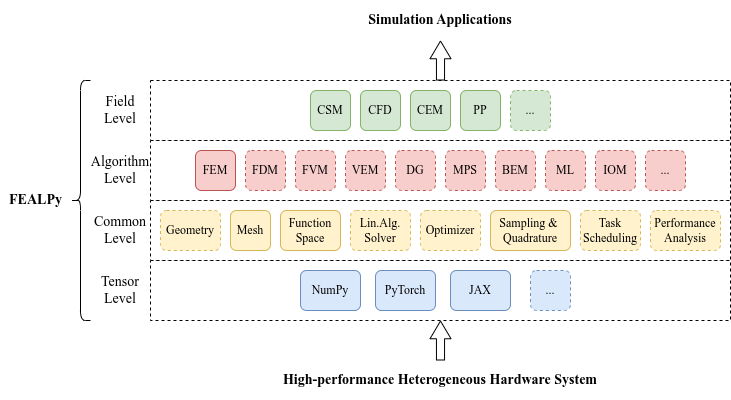
\includegraphics[width=0.8\textwidth]{figures/fealpy_structure.png}
	\caption{The layered architecture of FEALPy, comprising tensor, common, algorithm, and field levels, progressing from low-level functionalities to high-level applications. Modules in dashed boxes are under development.}
	\label{fs:fig1}
\end{figure}
\vspace{-0.5ex} % 可调节

Specifically, the functions of each layer are as follows:
\begin{enumerate} 
	\item \textbf{Tensor level}: Provides core tensor operations and manages backends (NumPy, PyTorch, JAX) via the Tensor Backend Manager, supporting SOPTX’s multi-backend switching. It also enables automatic differentiation (AD) in PyTorch and JAX, simplifying sensitivity computations in topology optimization (TO).
	\item \textbf{Common level}: Includes mesh generation and finite element spaces, supporting rapid construction of meshes and function spaces for finite element analysis in SOPTX.
	\item \textbf{Algorithm level}: Encompasses solvers and optimization algorithms, offering efficient and stable computational support for SOPTX’s optimization methods.
	\item \textbf{Field level}: Targets specific physical problems (e.g., linear elasticity), enabling SOPTX to address diverse TO problems, such as compliance minimization under volume constraints, with tailored application support.
\end{enumerate}
This layered design ensures FEALPy’s functionality, extensibility, and performance, with the Tensor Backend Manager abstracting backend differences to enhance user focus on algorithms and applications.

\subsection{SOPTX Architecture Design}
The SOPTX framework is positioned within the field level of FEALPy’s layered architecture, targeting structural topology optimization (STO) applications. SOPTX fully inherits and extends FEALPy’s \textit{Tensor Backend Manager}, diverse numerical algorithm components, and general-purpose mesh and geometry handling capabilities. This design not only ensures flexibility and extensibility, but also significantly improves computational efficiency for TO problems.

As shown in Figure~\ref{fs:fig2}, SOPTX adopts a modular architecture consisting of four primary components: the material, solver, filter, and optimizer modules. These components communicate and share data through well-defined interfaces, forming a loosely coupled and easily extensible multi-backend framework for TO.
\vspace{-0.5ex} % 可调节
\begin{figure}[htp]
	\centering
	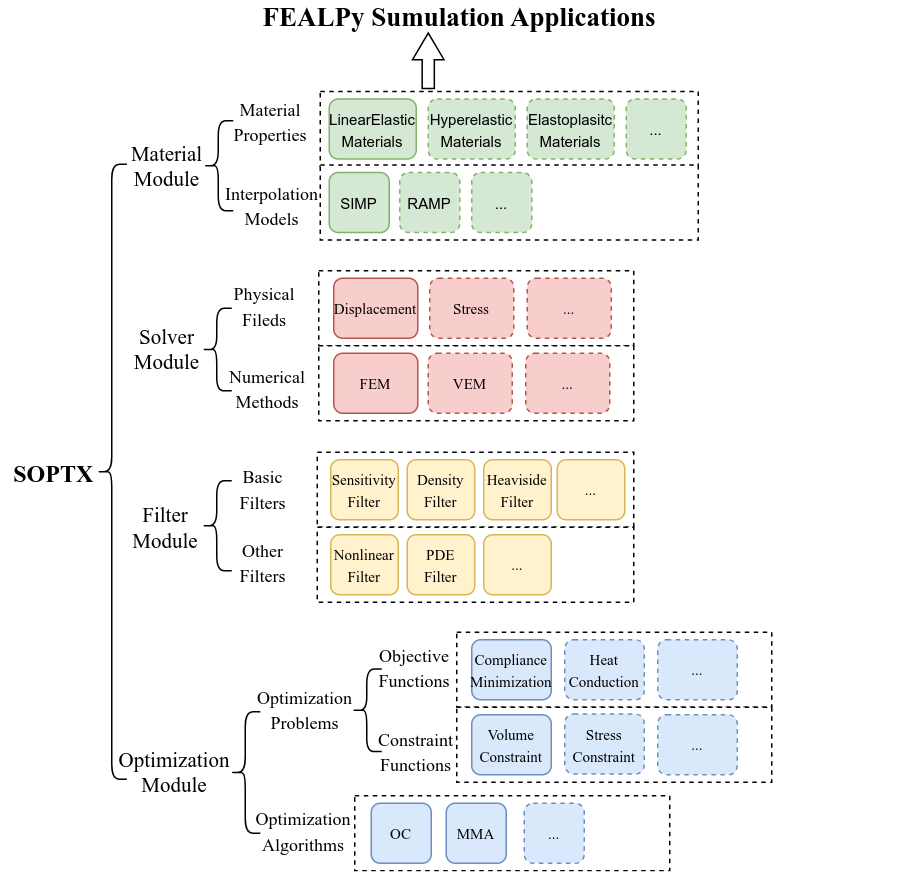
\includegraphics[width=0.7\textwidth]{figures/soptx_structure.png} % 保证 0.75
	\caption{The modular architecture of SOPTX, consisting of material, solver, filter, and optimization modules. The material module serves as the foundation, while the solver and filter modules manage intermediate computations, collectively supporting the optimization module. Components in dashed boxes are under development.}
	\label{fs:fig2}
\end{figure}
\vspace{-0.5ex} % 可调节

\subsubsection{Material Module}
The material module in SOPTX currently focuses on linear elastic materials, extending FEALPy’s implementation with TO-specific interfaces for computing Lamé constants, elasticity matrices, and strain matrices. It implements the Solid Isotropic Material with Penalization (SIMP) model, typically using a penalization factor $p = 3$, to transform continuous density fields into discrete material distributions. The module’s abstract interface design ensures extensibility, allowing future support for models like the Rational Approximation of Material Properties (RAMP) or complex behaviors such as anisotropy, hyperelasticity, and elastoplasticity through subclassing.

The module encapsulates the interpolation, update, and evaluation of elastic constants within a unified interface, providing essential material data for downstream modules. Its key functional interfaces include:
\begin{enumerate}
	\item Computing elasticity tensors from density fields for the solver module.
	\item Efficient batch updates of material properties for iterative optimization.
	\item Providing base material parameters (e.g., elastic constants) for optimization.
\end{enumerate}

These interfaces ensure consistent backend compatibility and optimized performance. The material module bridges physical modeling and numerical optimization, maintaining independence while supplying essential data throughout the TO workflow. Its modular design simplifies current linear elasticity solutions and provides a flexible foundation for future material model extensions.

\subsubsection{Solver Module}
The solver module forms the computational core of the SOPTX framework, tasked with solving physical field problems (e.g., displacement fields) based on given material properties, boundary conditions, and external loads. Its design philosophy centers on creating an efficient, flexible, and backend-independent solver engine to address the demands of repeatedly solving large-scale linear systems in TO. To achieve this, the module enhances computational efficiency through optimized matrix assembly, intelligent caching, and multi-backend acceleration, with support for backends such as NumPy, PyTorch, and JAX.

In its current version, SOPTX primarily adopts the finite element method (FEM) to solve linear elasticity equations, leveraging functionalities from FEALPy’s finite element module. The key features of the solver module include:
\begin{enumerate}
	\item \textbf{Dimensional and element adaptability}: It supports various spatial dimensions, element types, and boundary conditions, with the current version representing the density field as piecewise constant per element and the displacement field using linear finite elements to ensure stability and efficiency
	\item \textbf{Efficient numerical strategies}: The module implements a fast matrix assembly technique that separates element-independent and element-dependent components to eliminate redundant computations. Additionally, it incorporates symbolic integration to boost efficiency by precomputing exact expressions.
	\item \textbf{Multiple solution strategies}: It provides both direct solvers (e.g., MUMPS) and iterative solvers (e.g., Conjugate Gradient, CG), with automatic optimization tailored to the backend, such as utilizing GPU acceleration on PyTorch and JAX.
\end{enumerate}

The solver module is designed with strong extensibility, allowing for future incorporation of additional physical fields (e.g., stress fields) and numerical methods (e.g., Virtual Element Method), as well as adaptation to nonlinear mechanics and multiphysics coupling scenarios.

Within the SOPTX framework, the solver module acts as a bridge between physical analysis and optimization computation through the following interactions:
\begin{enumerate}
	\item \textbf{Interaction with the material module}: It receives material properties, such as elasticity matrices, via standardized interfaces, ensuring the solver remains independent of specific material interpolation schemes.
	\item \textbf{Output to the optimization module}: It supplies the displacement field for objective function evaluation and the stiffness matrix for sensitivity analysis.
	\item \textbf{Result reuse}: It employs an intelligent caching mechanism to avoid recomputing invariant components, substantially reducing computational overhead.
\end{enumerate}
Through its modular design and well-defined interfaces, the solver module efficiently conducts physical field computations, delivering critical support to the TO process while ensuring consistency and high performance across multiple backends.

\subsubsection{Filter Module}
The filter module in SOPTX is a cornerstone of TO, tasked with processing design variables and applying regularization techniques. Its primary functions are to mitigate numerical instabilities, such as checkerboarding and mesh dependency, and to improve the manufacturability of optimized structures. Adhering to the framework’s loosely coupled design, the filter module operates as an independent unit with efficient data exchange across modules. It offers a unified interface supporting multiple computational backends, with backend-specific optimizations ensuring high computational efficiency.

The module implements three key filtering techniques:
\begin{enumerate}
	\item \textbf{Sensitivity filtering}: Applies weighted averaging to objective function sensitivities, effectively suppressing checkerboard patterns.
	\item \textbf{Density filtering}: Maps raw design variables to physical densities, overcoming locality limitations of sensitivity filtering.
	\item \textbf{Heaviside projection filtering}: Enhances density filtering with a smoothed Heaviside function, driving intermediate densities toward 0 or 1 for distinct black-and-white designs.
\end{enumerate}

The module employs a KD-tree-based neighborhood search to construct filtering matrices, enabling efficient regularization on unstructured meshes and complex geometries. Optimization strategies, such as precomputed neighborhoods and sparse matrix representations, ensure scalability for large-scale TO problems.

The filter module is highly extensible. Users can subclass the base filter class to implement custom algorithms (e.g., nonlinear filters or PDE-based filters), inheriting multi-backend compatibility seamlessly. Additionally, the framework supports chained filter combinations, allowing tailored regularization strategies for diverse optimization needs.

The filter module interacts with other components in the following ways:
\begin{enumerate}
	\item \textbf{Solver Module}: Receives raw design variables and outputs filtered physical densities.
	\item \textbf{Optimization Module}: Filters unprocessed sensitivities to maintain numerical stability during optimization
	\item \textbf{Material Module}: Provides filtered densities for material interpolation, forming a streamlined data flow:
	\begin{equation*}
		\text{design variables} \to \text{filtering} \to \text{physical density} \to \text{material properties} \to \text{physical response}.
	\end{equation*}
\end{enumerate}

Through its modular and extensible design, the filter module not only resolves numerical challenges in TO but also lays a robust foundation for advanced regularization, facilitating high-quality, manufacturable structural designs within the SOPTX framework.

\subsubsection{Optimization Module}
The optimization module serves as the computational core of the SOPTX framework, tasked with formulating and solving mathematical optimization problems by integrating physical field solutions with user-defined objectives. It collaborates seamlessly with the material, solver, and filter modules to drive the topology optimization (TO) pipeline. Adhering to the framework’s multi-backend design, it offers a unified interface across NumPy, PyTorch, and JAX, leveraging backend-specific optimizations, such as GPU acceleration in PyTorch and JAX, for enhanced performance.

The module currently focuses on compliance minimization under volume constraints, a foundational problem in TO, and supports two mainstream algorithms: Optimality Criteria (OC), a lightweight method for volume-constrained problems, and Method of Moving Asymptotes (MMA), based on Svanberg’s 2007 formulation~\cite{Svanberg2007MmaAG}, adapted for multi-backend compatibility and optimized for efficiency.

The design of the optimization module follows two core principles
\vspace{-0.5ex} % 可调节
\begin{enumerate}
	\item \textbf{Decoupling of problem and algorithm}: The optimization problem (e.g., objectives, constraints, sensitivities) is separated from the solving algorithm, enabling flexible pairing of formulations and solvers.
	\item \textbf{Dual-mode sensitivity}: Supports both manually derived sensitivities for transparency and AD in PyTorch or JAX for ease and scalability.
\end{enumerate}
\vspace{-0.5ex} % 可调节

The optimization module is designed with high extensibility, allowing users to
\vspace{-0.5ex} % 可调节
\begin{enumerate}
	\item \textbf{Custom problems}: Users can extend the module by subclassing the base problem class to introduce new objectives (e.g., heat conduction, compliant mechanisms) or constraints (e.g., stress, frequency).
	\item \textbf{Algorithm integration}: Additional algorithms, such as Sequential Quadratic Programming (SQP) or Sequential Linear Programming (SLP), can be incorporated modularly.
\end{enumerate}
\vspace{-0.5ex} % 可调节

The optimization module serves as a central hub within the SOPTX framework, coordinating closely with other modules through the following interactions
\vspace{-0.5ex} % 可调节
\begin{enumerate}
	\item \textbf{Solver Module}: Utilizes physical outputs (e.g., displacement fields, stiffness matrices) to compute objectives and sensitivities.
	\item \textbf{Filter Module}: Sends raw sensitivities for processing, receives filtered sensitivities for updates, and applies filtering to design variables to derive physical densities.
\end{enumerate}
\vspace{-0.5ex} % 可调节

With its modular and extensible architecture, the optimization module efficiently tackles classical TO problems while laying a versatile foundation for advanced multiphysics optimization. It acts as the decision-making hub of SOPTX, balancing performance, flexibility, and user adaptability.

\subsection{Multi-Backend Switching}
In structural topology optimization (STO), computational performance is a central concern in both research and engineering. To meet diverse computational demands, the SOPTX framework builds upon FEALPy to implement a flexible multi-backend architecture. This allows seamless switching between tensor computation backends such as NumPy, PyTorch, and JAX, enhancing software applicability, efficiency, portability, and flexibility across various hardware and software platforms.

Specifically, each backend offers distinct advantages for different scenarios
\vspace{-0.5ex} % 可调节
\begin{itemize} 
	\item \textbf{NumPy backend}: Ideal for small-scale tasks and rapid prototyping, providing stable performance and efficient memory management on standard CPU platforms.
	\item \textbf{PyTorch and JAX backends}: Both support GPU acceleration and AD, making them suitable for large-scale or high-dimensional problems. AD streamlines sensitivity analysis, while JAX offers just-in-time (JIT) compilation and automatic vectorization, which can further enhance performance on GPU platforms.
\end{itemize}
\vspace{-0.5ex} % 可调节

\section{Getting Started with SOPTX}
This chapter provides installation instructions and usage guidance for SOPTX, enabling readers to quickly grasp the framework's operations and apply it to topology optimization (TO) tasks. Built on FEALPy, SOPTX leverages a multi-backend switching mechanism and modular design to deliver an efficient and flexible computational environment. The chapter is structured into two sections: first, a detailed guide on installing SOPTX and its dependency FEALPy, ensuring proper configuration of the development environment; second, a demonstration of SOPTX's workflow through a classical 2D cantilever beam compliance minimization example.

\subsection{Software Installation}
SOPTX is a TO toolkit built on top of FEALPy, an intelligent CAE simulation engine that provides numerical computing capabilities. Installing FEALPy is required before SOPTX. For flexibility and the latest features, install both from source. Ensure Git and Python are installed. Use a virtual environment to avoid dependency conflicts.

Core installation steps:
\vspace{-0.5ex} % 可调节
\begin{enumerate} 
	\item Clone the FEALPy repository from GitHub:
\vspace{-0.5ex} % 可调节
\begin{lstlisting}[language=bash]
git clone https://github.com/weihuayi/fealpy.git
\end{lstlisting}
\vspace{-0.5ex} % 可调节
	\item Change into the FEALPy directory and install it in editable mode:
\vspace{-0.5ex} % 可调节
\begin{lstlisting}[language=bash]
cd fealpy
pip install -e . 
\end{lstlisting}
\vspace{-0.5ex} % 可调节
	\item Similarly, install SOPTX:
\vspace{-0.5ex} % 可调节
\begin{lstlisting}[language=bash]
git clone https://github.com:weihuayi/soptx.git
cd soptx
pip install -e . 
\end{lstlisting}
\vspace{-0.5ex} % 可调节
\end{enumerate}
\vspace{-0.5ex} % 可调节

For the complete installation guide, please refer to the official documentation at: \url{https://github.com/weihuayi/fealpy}.

\subsection{Example: 2D Cantilever Beam}\label{sec:exp_canti_beam}
We use a popular compliance minimization benchmark to demonstrate the usage of SOPTX: minimizing the structural compliance of a cantilever beam under tip loading (see Figure~\ref{fig:cantilever})~\cite{bendsoe2013topology}. The left end of the beam is fixed, and a downward concentrated load $T = -1$ is applied to the bottom of the right end. A $160 \times 100$ uniform quadrilateral mesh is used. The target volume fraction is set to 0.4, with material properties $E = 1$ and $\nu = 0.3$. The penalization factor is $p = 3$, and the sensitivity filter radius is $r = 6.0$, which matches the mesh element size to ensure structural smoothness and eliminate checkerboard patterns.
\vspace{-2ex} % 可调节
\begin{figure}[htp]
	\centering
	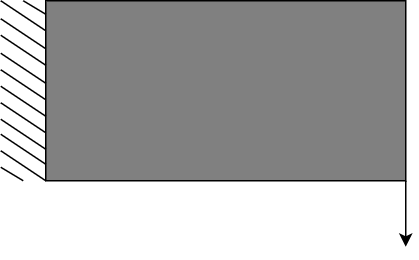
\includegraphics[width=0.5\textwidth]{figures/cantilever_2d.png}
	\caption{Cantilever beam geometry: fixed on the left, with a downward concentrated load on the right.}
	\label{fig:cantilever}
\end{figure}
\vspace{-2ex} % 可调节

To begin, we import essential modules from FEALPy (backend, mesh, function spaces) and SOPTX (material, solver, filter, optimization), as shown in Code~\ref{code:mouldes_pde}. The partial differential equation (PDE) model for the cantilever beam, defined in \texttt{Cantilever2dData1} (see~\ref{sec:code_canti_2d}), specifies the geometry, load, and boundary conditions via standard SOPTX interfaces.

\vspace{-0.5ex} % 可调节
\begin{lstlisting}[language=python, caption={Module imports and PDE model}, label={code:mouldes_pde}]
from fealpy.backend import backend_manager as bm
from fealpy.mesh import UniformMesh2d
from fealpy.functionspace import LagrangeFESpace, TensorFunctionSpace

from soptx.material import DensityBasedMaterialConfig, DensityBasedMaterialInstance
from soptx.solver import ElasticFEMSolver, AssemblyMethod
from soptx.filter_ import SensitivityBasicFilter
from soptx.opt import ComplianceObjective, ComplianceConfig, VolumeConstraint, VolumeConfig
from soptx.opt import OCOptimizer
from soptx.pde import Cantilever2dData1

pde = Cantilever2dData1(xmin=0, xmax=160, ymin=0, ymax=100,	T = -1)
\end{lstlisting}
\vspace{-0.5ex} % 可调节

Next, we define the mesh and finite element spaces (Code~\ref{code:mesh_space}). The displacement field uses a first-order continuous Lagrange space, while the density field is represented in a zeroth-order discontinuous Lagrange space, aligning with typical TO discretizations.

\vspace{-0.5ex} % 可调节
\begin{lstlisting}[language=python, caption={Mesh and function space definitions}, label={code:mesh_space}]
mesh = UniformMesh2d(extent=[0, 160, 0, 100], h=[1, 1], origin=[0, 0])
space_C = LagrangeFESpace(mesh=mesh, p=1, ctype='C')
tensor_space_C = TensorFunctionSpace(scalar_space=space_C, shape=(-1, 2))
space_D = LagrangeFESpace(mesh=mesh, p=0, ctype='D')
\end{lstlisting}
\vspace{-0.5ex} % 可调节

The material module is then instantiated with the specified properties and SIMP interpolation model (Code~\ref{code:material}). This module handles material property computations based on the density field.

\vspace{-0.5ex} % 可调节
\begin{lstlisting}[language=python, caption={Material module}, label={code:material}]
material_config = DensityBasedMaterialConfig(
		elastic_modulus=1.0, minimal_modulus=1e-9, 
		poisson_ratio=0.3, plane_assumption="plane_stress",  
		interpolation_model="SIMP", penalty_factor=3.0)
materials = DensityBasedMaterialInstance(config=material_config)
\end{lstlisting}
\vspace{-0.5ex} % 可调节

Subsequently, the solver module is initialized with the material module, PDE model, standard matrix assembly, and a direct solver (MUMPS), as shown in Code~\ref{code:solver_filter}. A sensitivity filter with radius $r = 6.0$ is also set up to regularize the optimization.

\vspace{-0.5ex} % 可调节
\begin{lstlisting}[language=python, caption={Solver and filter module}, label={code:solver_filter}] 
solver = ElasticFEMSolver(materials=materials,
			tensor_space=tensor_space_C, pde=pde,
			assembly_method=AssemblyMethod.STANDARD,
			solver_type='direct',
			solver_params={'solver_type': 'mumps'})
sens_filter = SensitivityBasicFilter(mesh=mesh, rmin=6.0)
\end{lstlisting}
\vspace{-0.5ex} % 可调节

The optimization problem is defined by instantiating the compliance objective and volume constraint classes, followed by configuring the Optimality Criteria (OC) optimizer with a maximum of 200 iterations and a convergence tolerance of 0.01 (Code~\ref{code:optimizer}).

\vspace{-0.5ex} % 可调节
\begin{lstlisting}[language=python, caption={Optimization module}, label={code:optimizer}]
objective = ComplianceObjective(solver=solver)
constraint = VolumeConstraint(solver=solver, volume_fraction=0.4)
optimizer = OCOptimizer(objective=objective,
			constraint=constraint, filter=sens_filter,
			options={'max_iterations': 200, 'tolerance': 0.01})
\end{lstlisting}
\vspace{-0.5ex} % 可调节

Finally, the initial density field is uniformly set to the target volume fraction, and the optimization is executed. Results are saved, and convergence history is plotted (Code~\ref{code:main_post}).

\vspace{-0.5ex} % 可调节
\begin{lstlisting}[language=python, caption={Main program and post-processing}, label={code:main_post}]
if __name__ == "__main__":
	@cartesian
	def density_func(x):
		val = config.init_volume_fraction * bm.ones(x.shape[0], **kwargs)
		return val
	rho = space_D.interpolate(u=density_func)
	rho_opt, history = optimizer.optimize(rho=rho[:])
	
	from soptx.opt import save_optimization_history, plot_optimization_history
	save_optimization_history(mesh, history)
	plot_optimization_history(history)
\end{lstlisting}
\vspace{-0.5ex} % 可调节

Figure~\ref{fig:canti_04_convergence} shows the convergence histories of the compliance $c(\rho)$ and the volume fraction $v(\rho)$ for an initial density of 0.4. After running the code, Figure~\ref{fig:canti_04_convergence} shows the convergence histories of the compliance $c(\rho)$ and the volume fraction $v(\rho)$. Compliance decreases rapidly from its initial value of approximately 500 to around 100 in the first 10 iterations, converging by iteration 57. The volume fraction remains stably around 0.4, with only minor fluctuations.

\vspace{-2ex} % 可调节
\begin{figure}[htp]
	\centering
	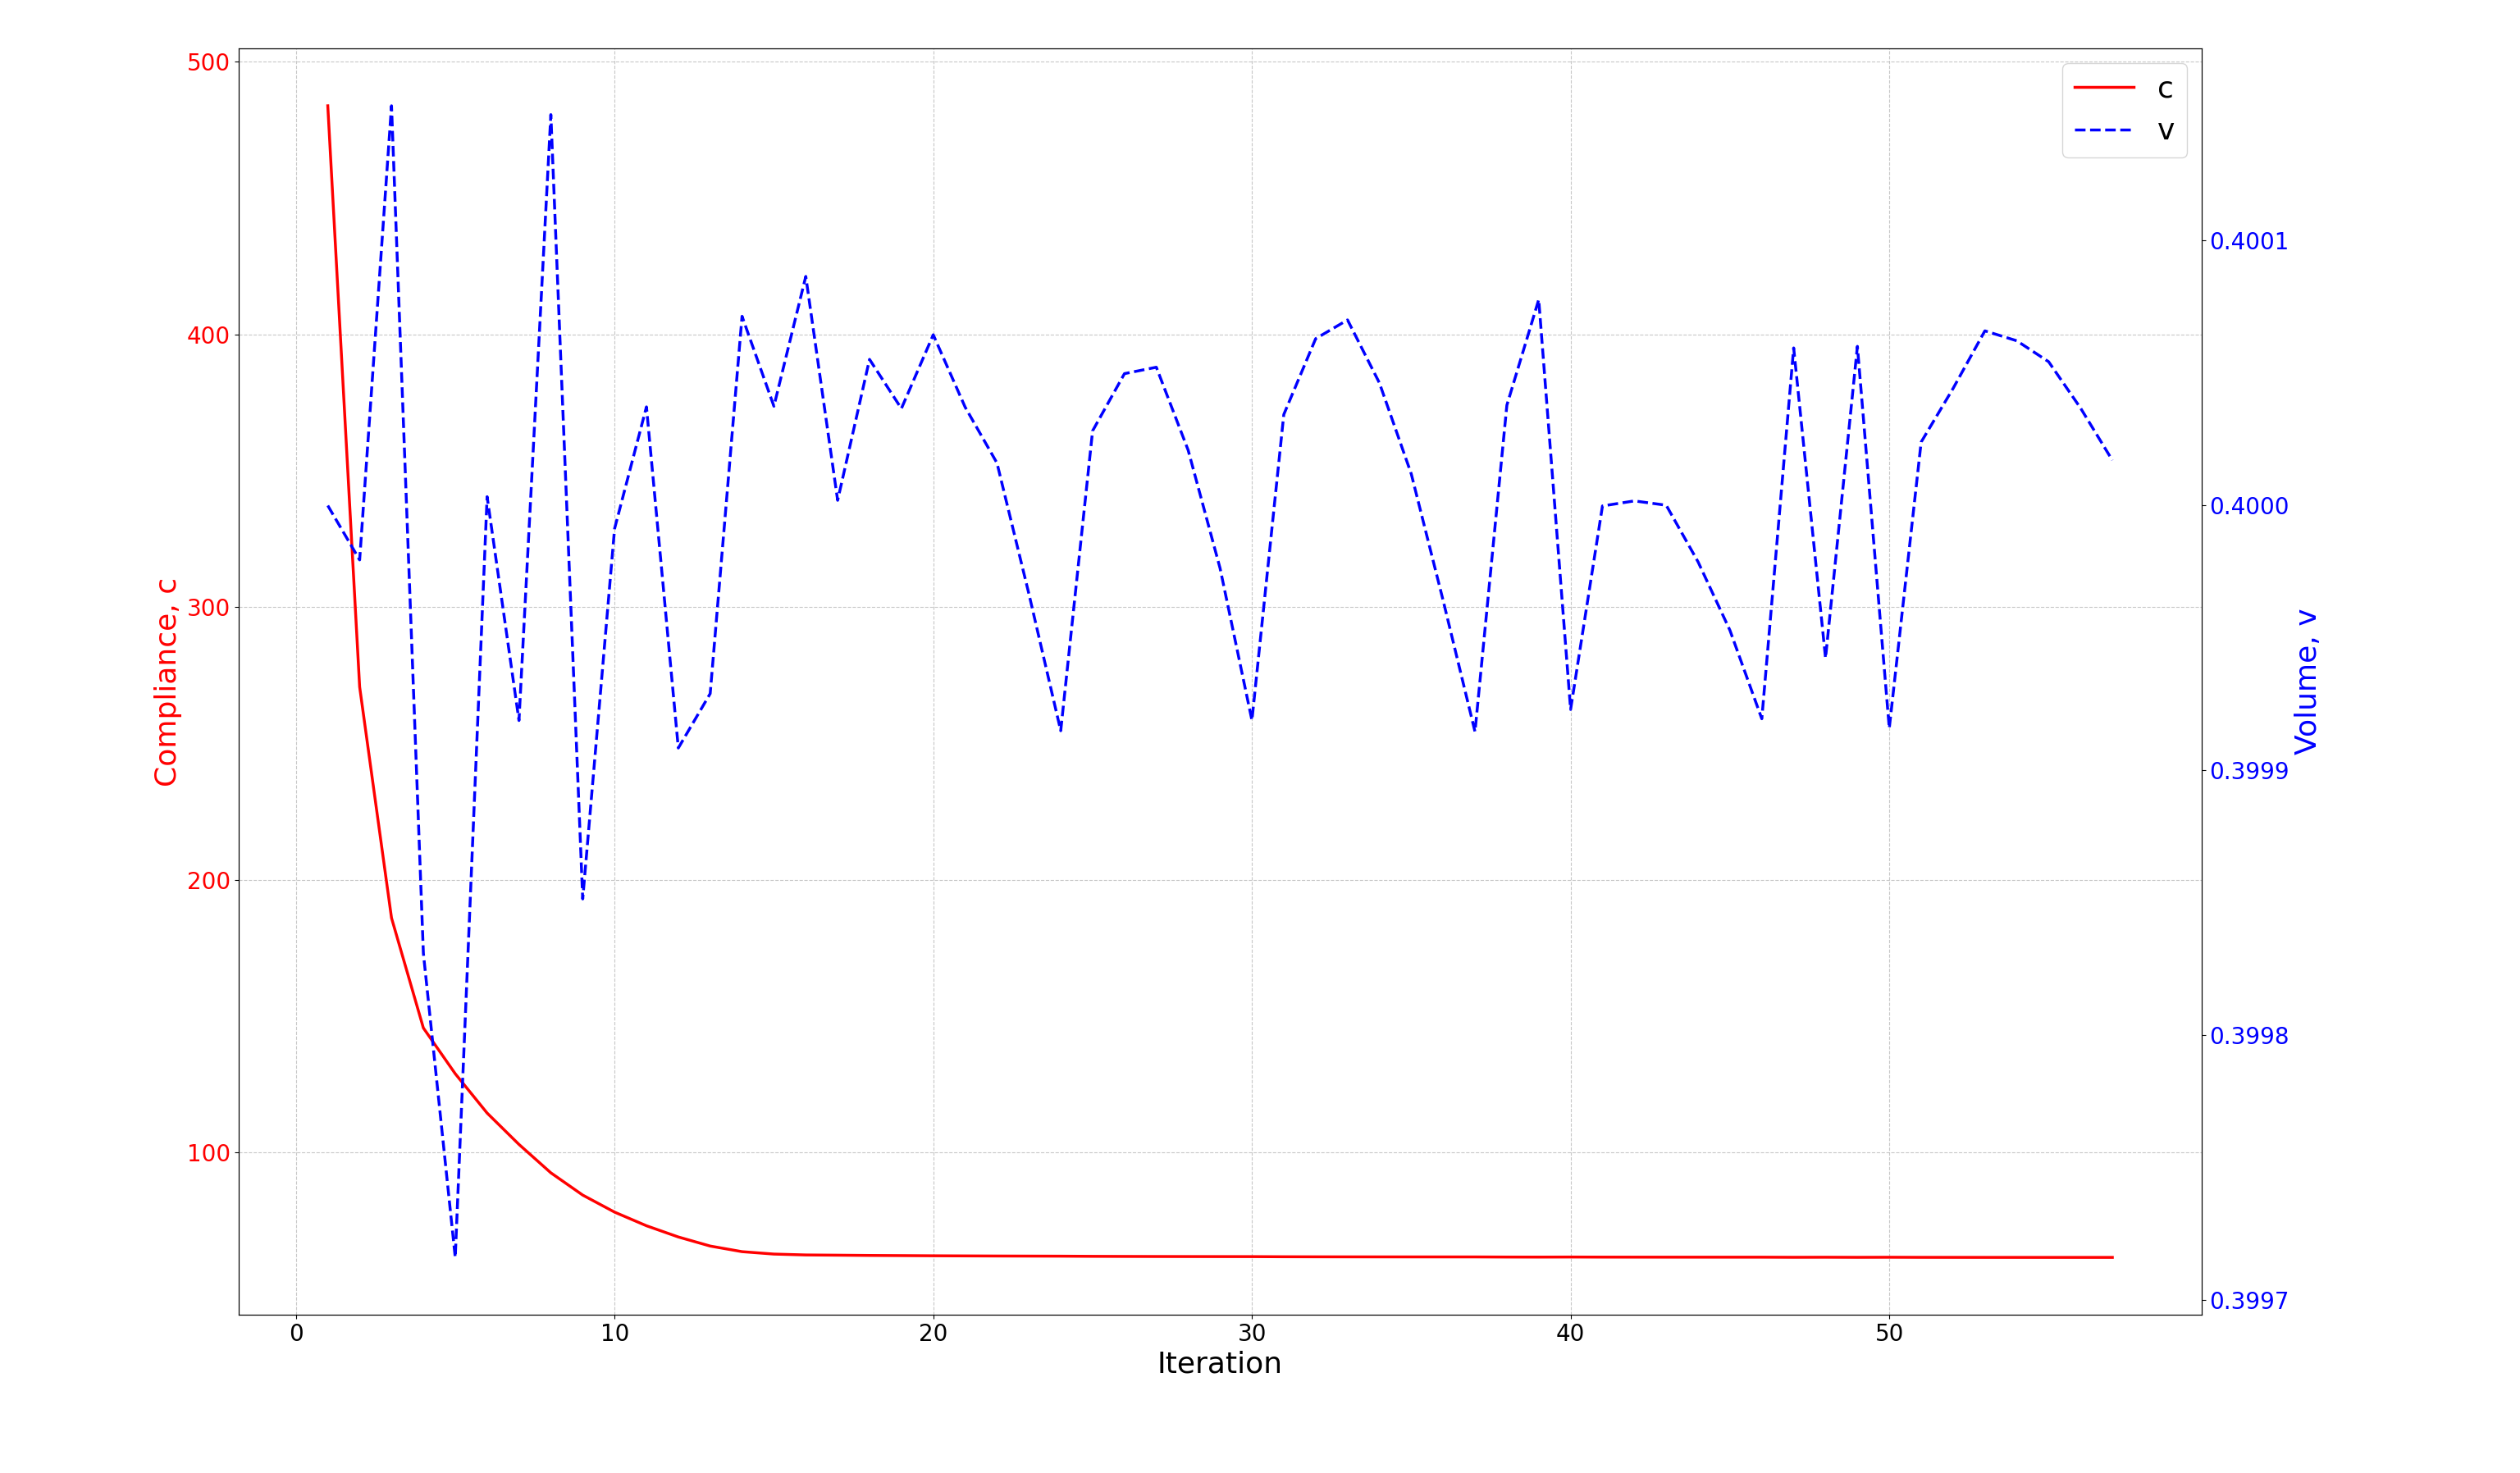
\includegraphics[width=0.85\textwidth]{figures/cantilever_2d_04_convergence.png}
	\caption{Convergence histories of the compliance $c(\rho)$ and volume fraction $v(\rho)$ for the 2D cantilever beam initialized with a uniform density of 0.4.}
	\label{fig:canti_04_convergence}
\end{figure}
\vspace{-2ex} % 可调节

Figure~\ref{fig:canti_04_all} displays the resulting topologies at iterations 3, 30, and 57.

\vspace{-2ex} % 可调节
\begin{figure}[htp]
	\centering
	\subfloat[$c(\rho)=145.5753,~v(\rho)=0.3998$]{
		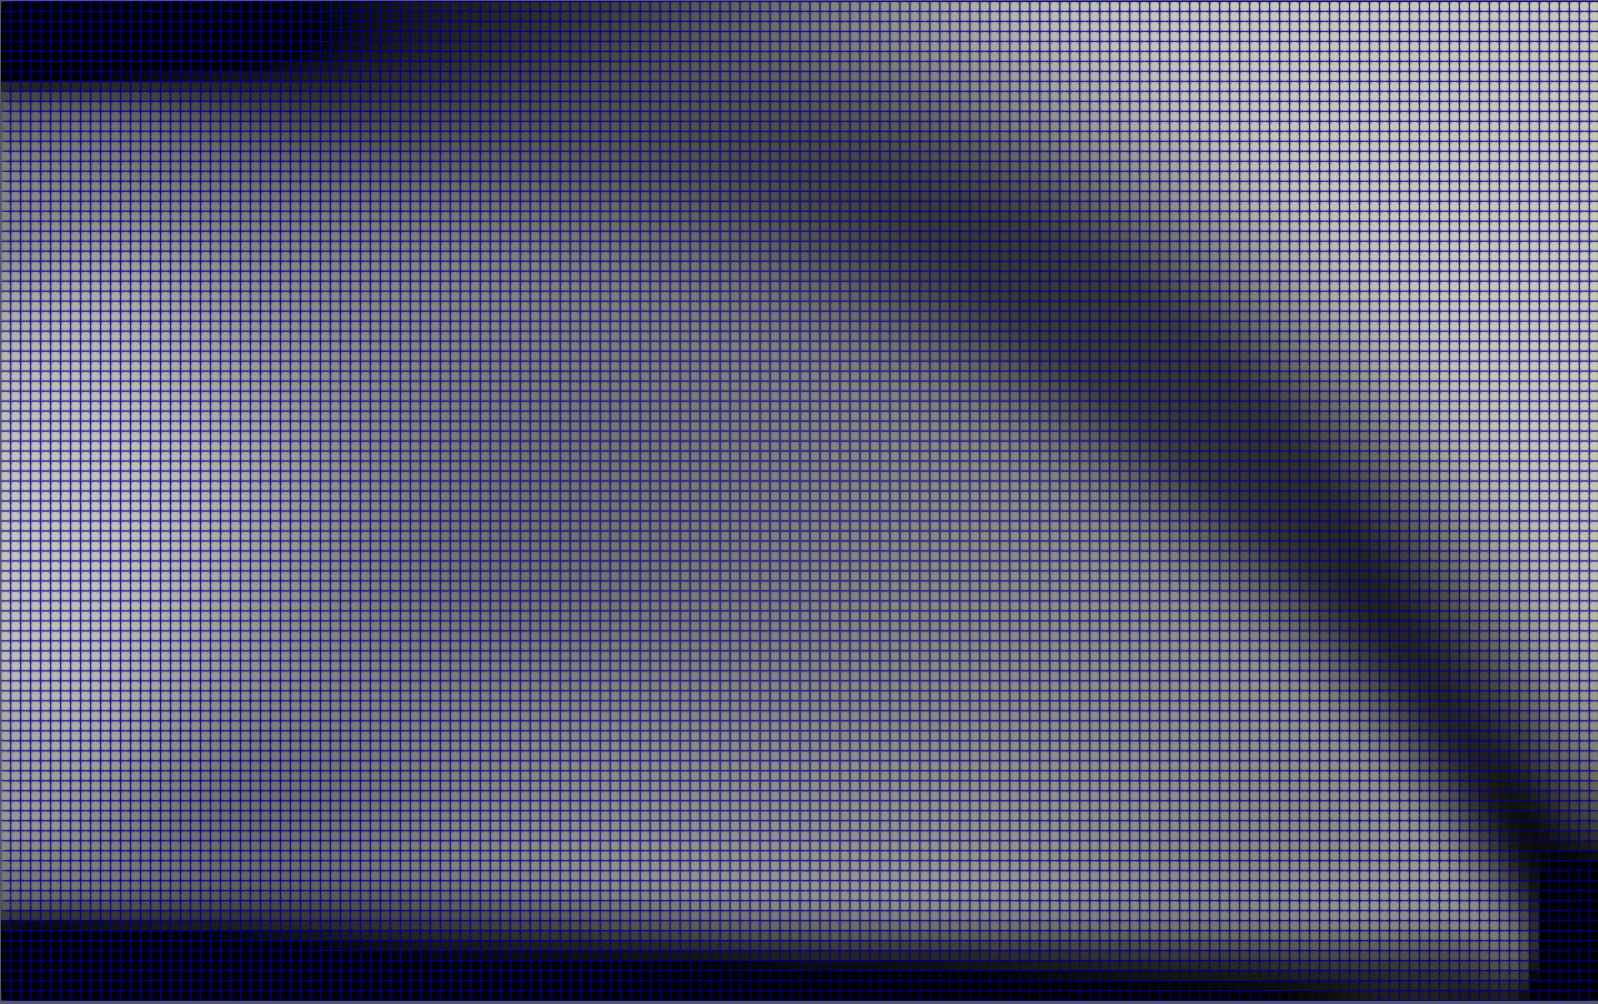
\includegraphics[width=0.32\textwidth]{figures/cantilever_2d_04_1.png}
		\label{fig:canti_04_1}
	}
	\subfloat[$c(\rho)=61.7084,~v(\rho)=0.3999$]{
		
\includegraphics[width=0.32\textwidth]{figures/cantilever_2d_04_2.png}
		\label{fig:canti_04_2}
	}
	\subfloat[$c(\rho)=61.4208,~v(\rho)=0.4000$]{
		
\includegraphics[width=0.32\textwidth]{figures/cantilever_2d_04_3.png}
		\label{fig:canti_04_3}
	}
	\caption{Topology layouts at iterations 3, 30, and 57 during the optimization process. Each subfigure also reports the corresponding compliance and volume fraction values.}
	\label{fig:canti_04_all}
\end{figure}
\vspace{-2ex} % 可调节

Figure~\ref{fig:canti_1_convergence} illustrates the convergence behavior for an initial density of 1. The volume fraction decreases from 1 to 0.4 within 5 iterations, while compliance initially increases to around 500 before decreasing to convergence at iteration 60. This process requires slightly more iterations due to the initial adjustment to meet the volume constraint.

\vspace{-2ex} % 可调节
\begin{figure}[htp]
	\centering
	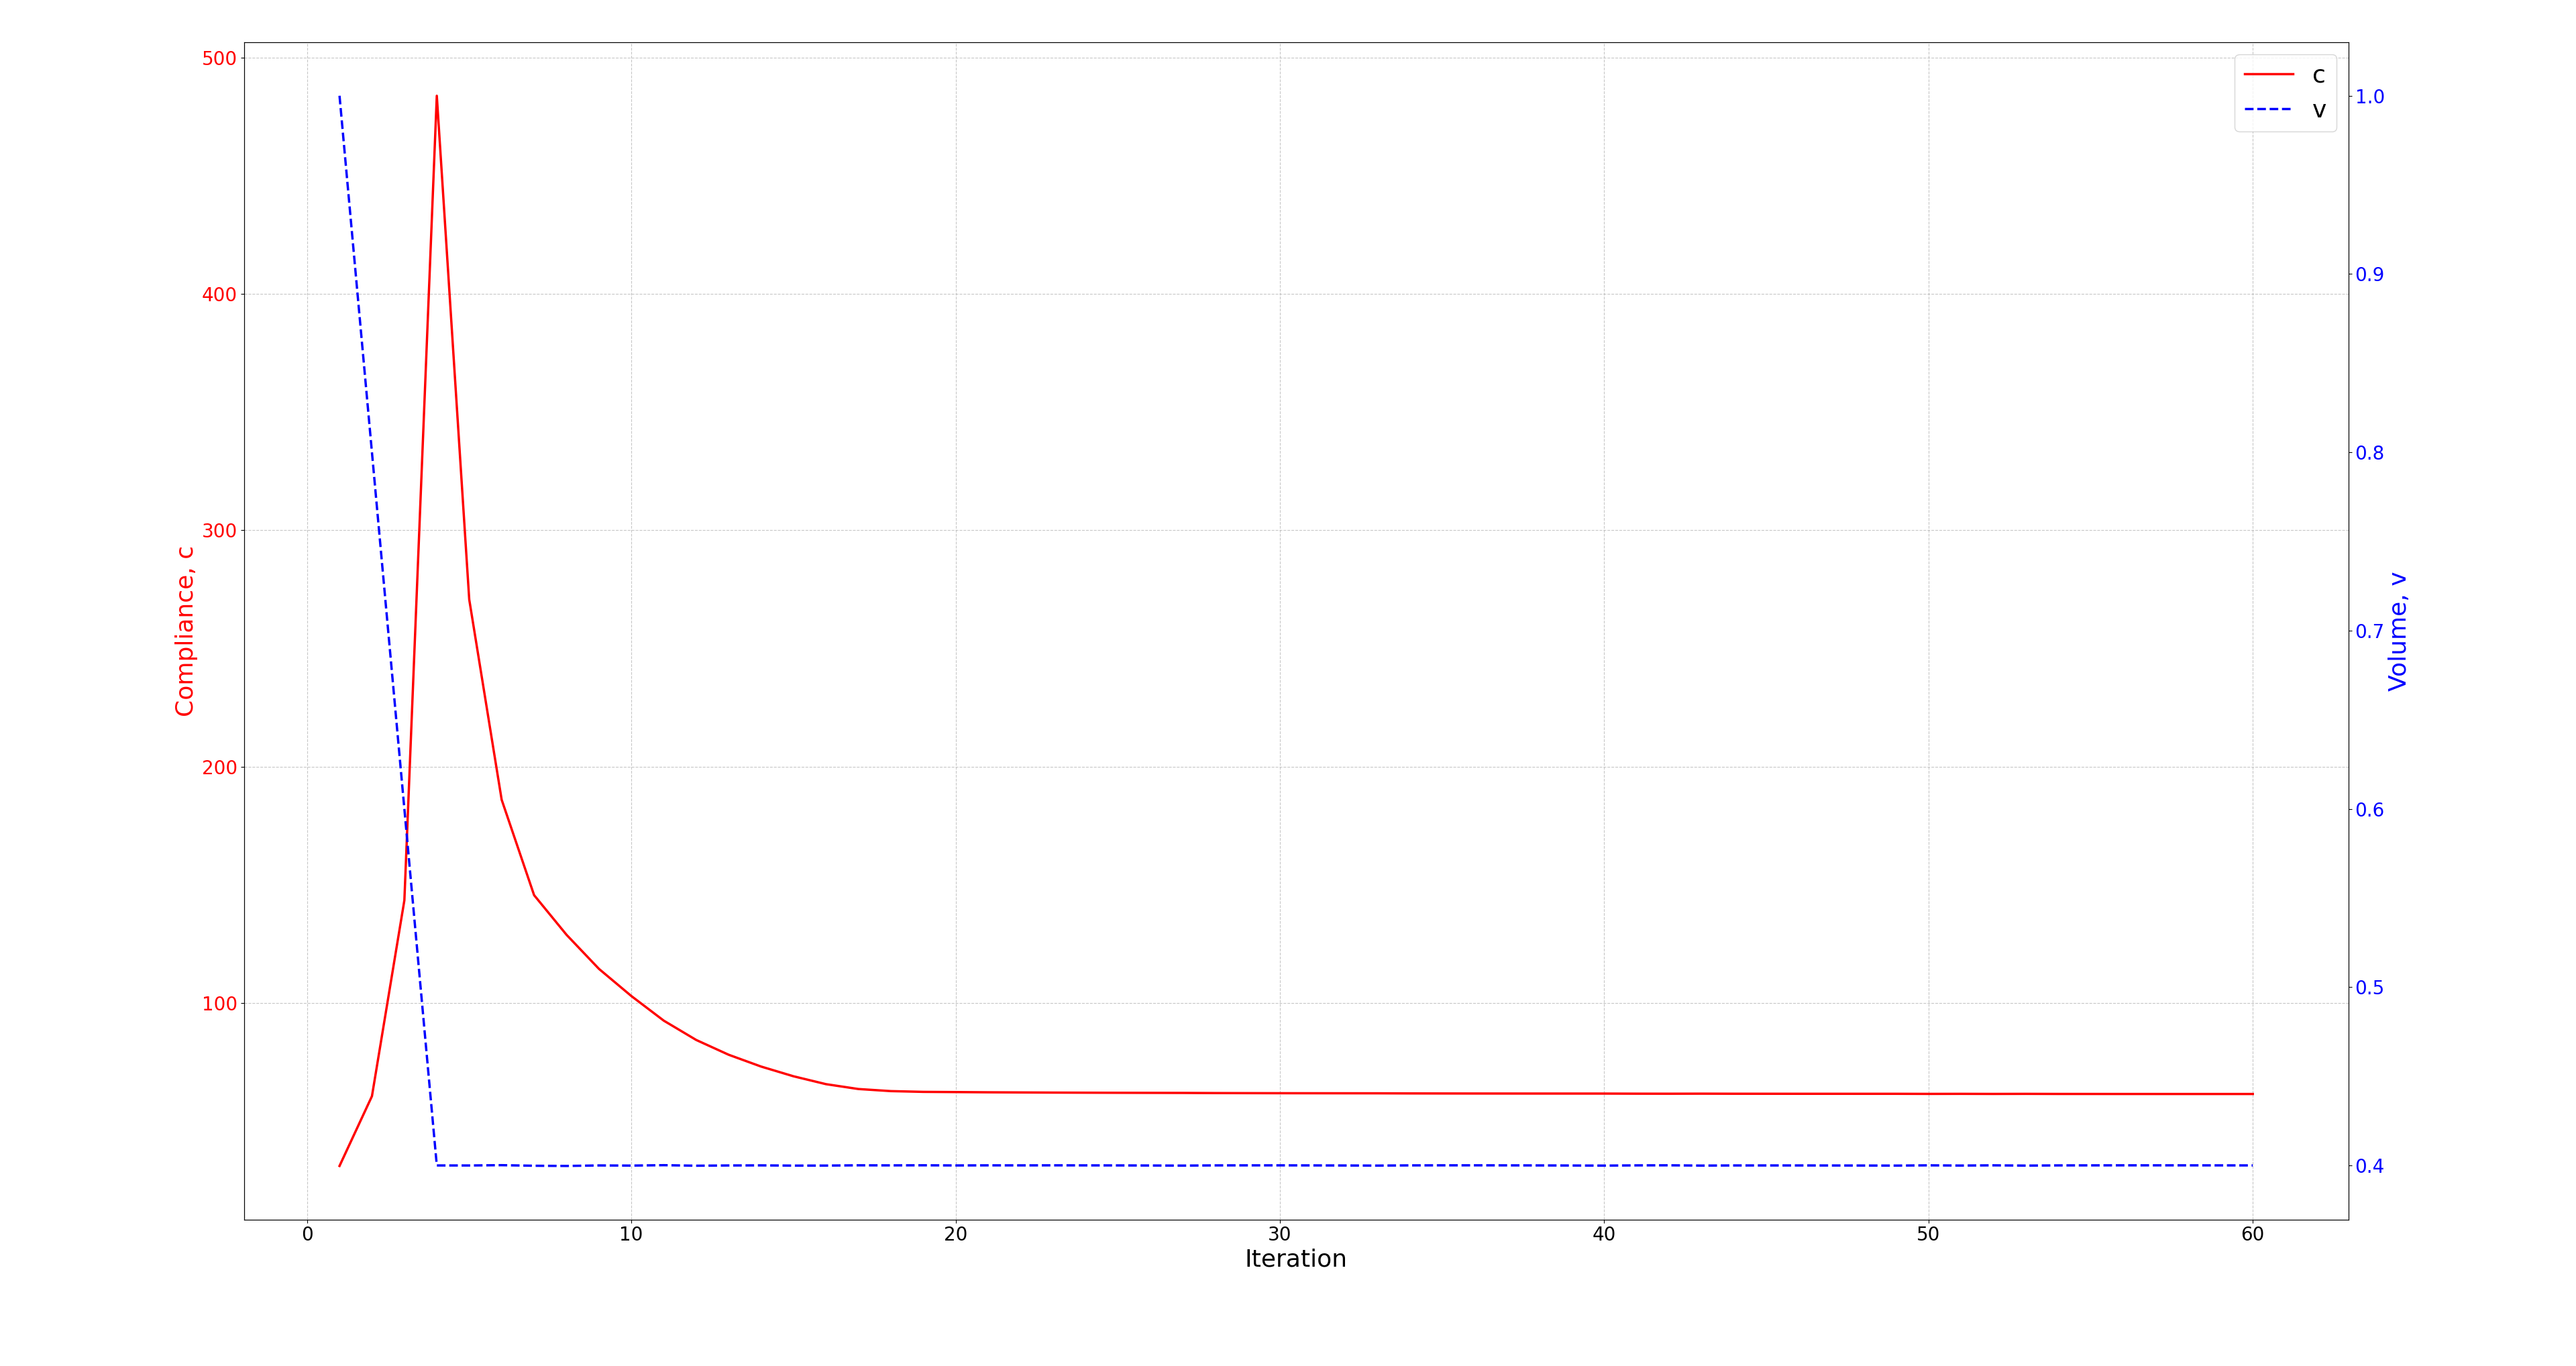
\includegraphics[width=0.85\textwidth]{figures/cantilever_2d_1_convergence.png}
	\caption{Convergence histories of the compliance $c(\rho)$ and volume fraction $v(\rho)$ for the 2D cantilever beam with an initial density of $1$.}
	\label{fig:canti_1_convergence}
\end{figure}
\vspace{-2ex} % 可调节

Figure~\ref{fig:canti_1_all} shows the topology layouts at iterations 6, 33, and 60.

\vspace{-2ex} % 可调节
\begin{figure}[htp]
	\centering
	\subfloat[$c(\rho)=185.9530,~v(\rho)=0.4002$]{
		
\includegraphics[width=0.32\textwidth]{figures/cantilever_2d_1_1.png}
		\label{fig:canti_1_1}
	}
	\subfloat[$c(\rho)=61.7084,~v(\rho)=0.3999$]{
		
\includegraphics[width=0.32\textwidth]{figures/cantilever_2d_1_2.png}
		\label{fig:canti_1_2}
	}
	\subfloat[$c(\rho)=61.4208,~v(\rho)=0.4000$]{
		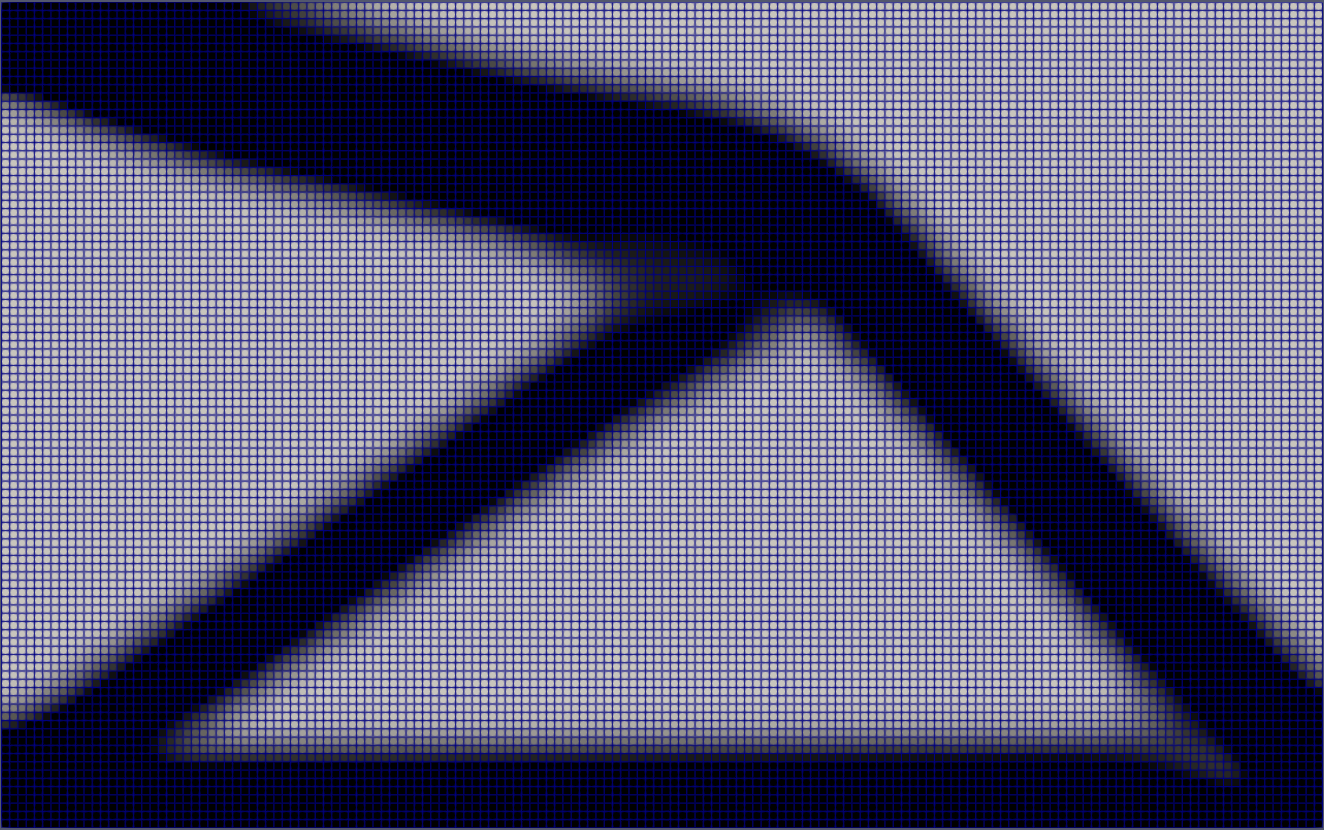
\includegraphics[width=0.32\textwidth]{figures/cantilever_2d_1_3.png}
		\label{fig:canti_1_3}
	}
	\caption{Topology layouts at iterations 6, 33, and 60 during the optimization process. Each subfigure includes the compliance and volume fraction values.}
	\label{fig:canti_1_all}
\end{figure}
\vspace{-2ex} % 可调节

These results highlight the robustness of SOPTX in handling different initial conditions and its efficiency in achieving convergence with the OC algorithm.

\section{Numerical Examples}
This chapter presents numerical examples to validate the SOPTX framework's capabilities in topology optimization (TO), spanning 2D MBB beam problems to 3D cantilever structures. These examples demonstrate SOPTX's versatility across diverse partial differential equation (PDE) models, meshes, filters, and algorithms, while showcasing advanced features like fast matrix assembly, automatic differentiation (AD), and multi-backend switching.

The chapter is organized as follows: Section~\ref{sec:exp_mbb_beam} tests robustness across mesh resolutions; Section 5.2 explores filtering effects; Section 5.3 introduces algorithm switching and an updated MMA optimizer; Section 5.4 extends to 3D TO; Section 5.5 quantifies matrix assembly gains; Section 5.6 highlights AD in sensitivity analysis; and Section 5.7 assesses multi-backend and graphics processing units (GPUs) acceleration benefits. These examples underscore SOPTX's strengths and its potential in research and engineering.

\subsection{MBB Beam}\label{sec:exp_mbb_beam}
As introduced, we first validate SOPTX using the MBB beam, a classical benchmark in TO widely used to assess optimization algorithms. This section minimizes the structural compliance of the MBB beam (see Figure~\ref{fig:mbb_beam}), demonstrating SOPTX's adaptability to various PDE models and meshes. The beam is hinged at the left edge and bottom right corner, with horizontal displacements constrained, and a downward load $T = -1$ applied at the upper left corner. The target volume fraction is 0.5, with material properties $E = 1$ and $\nu = 0.3$, penalization factor $p = 3$, and filter radius $r = 6.0$ to ensure smooth topology and suppress checkerboard patterns.
\vspace{-2ex} % 可调节
\begin{figure}[htp]
	\centering
	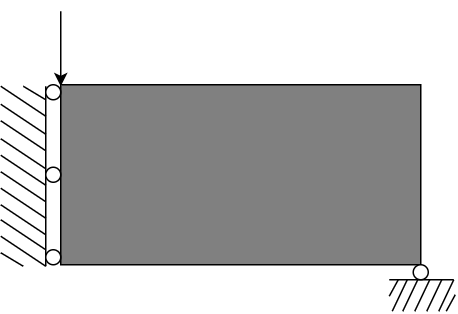
\includegraphics[width=0.6\textwidth]{figures/mbb_2d.png}
	\caption{Geometry of the MBB beam: hinged at the left edge and bottom right corner, with a downward concentrated load applied at the top left.}
	\label{fig:mbb_beam}
\end{figure}
\vspace{-2ex} % 可调节

Compared to the cantilever beam in Section~\ref{sec:exp_canti_beam}, SOPTX enables a seamless switch to the MBB beam problem. Users can modify the PDE model as follows:
\begin{lstlisting}[language=Python]
from soptx.pde import MBBBeam2dData1
pde = MBBBeam2dData1(xmin=0, xmax=150, ymin=0, ymax=50, T=-1)
\end{lstlisting}
The complete model definition is provided in Appendix~\ref{sec:code_mbb}.

To demonstrate SOPTX's adaptability across mesh types, we perform TO on a $150 \times 50$ uniform quadrilateral mesh and a triangular mesh, both initialized with a uniform material density equal to the target volume fraction 0.5. The triangular mesh is generated using:
\vspace{-0.5ex} % 可调节
\begin{lstlisting}[language=Python]
from fealpy.mesh import TriangleMesh
mesh = TriangleMesh.from_box([0, 150, 0, 50], nx=150, ny=50)
\end{lstlisting}
\vspace{-0.5ex} % 可调节

The optimized topologies, shown in Figure~\ref{fig:mbb_2d_all}, are consistent across both mesh types, with compliance and volume fraction differences below $1\%$. This consistency underscores SOPTX's mesh-independence and algorithmic robustness, facilitated by its modular design, which allows easy switching between PDE models and mesh configurations.

\vspace{-2ex} % 可调节
\begin{figure}[htp]
	\centering
	\subfloat[$c(\rho)=219.5199,~v(\rho)=0.5001$]{
		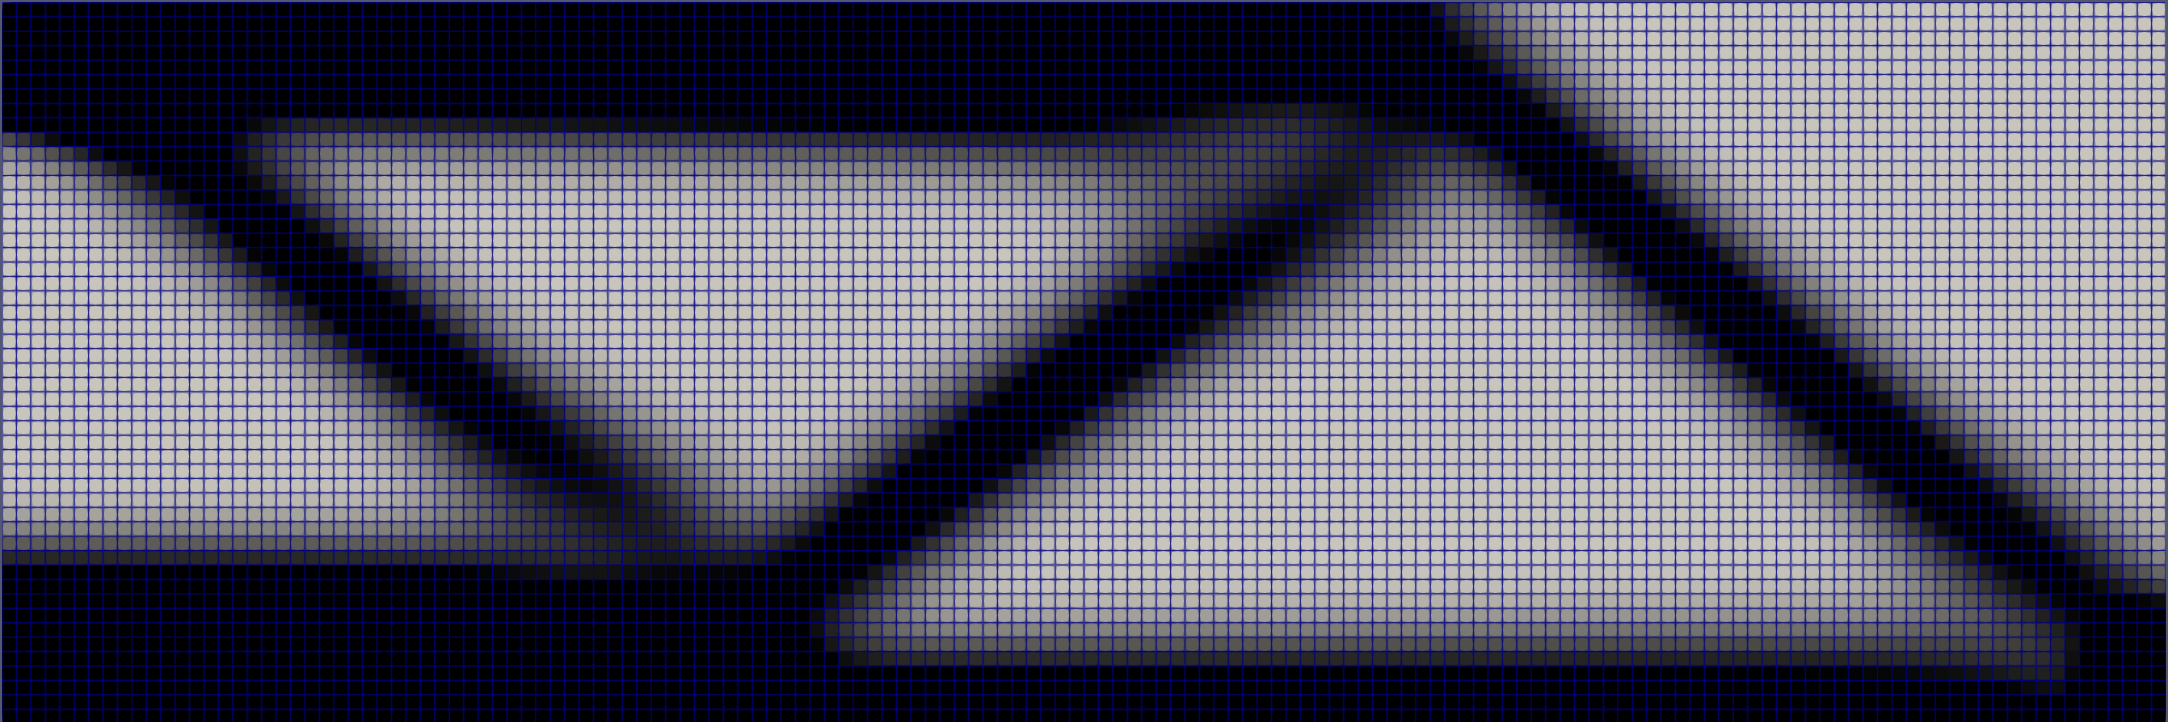
\includegraphics[width=0.5\textwidth]{figures/mbb_2d_u2.png}
		\label{fig:mbb_2d_u2}
	}
	\subfloat[$c(\rho)=217.6605,~v(\rho)=0.4999$]{
		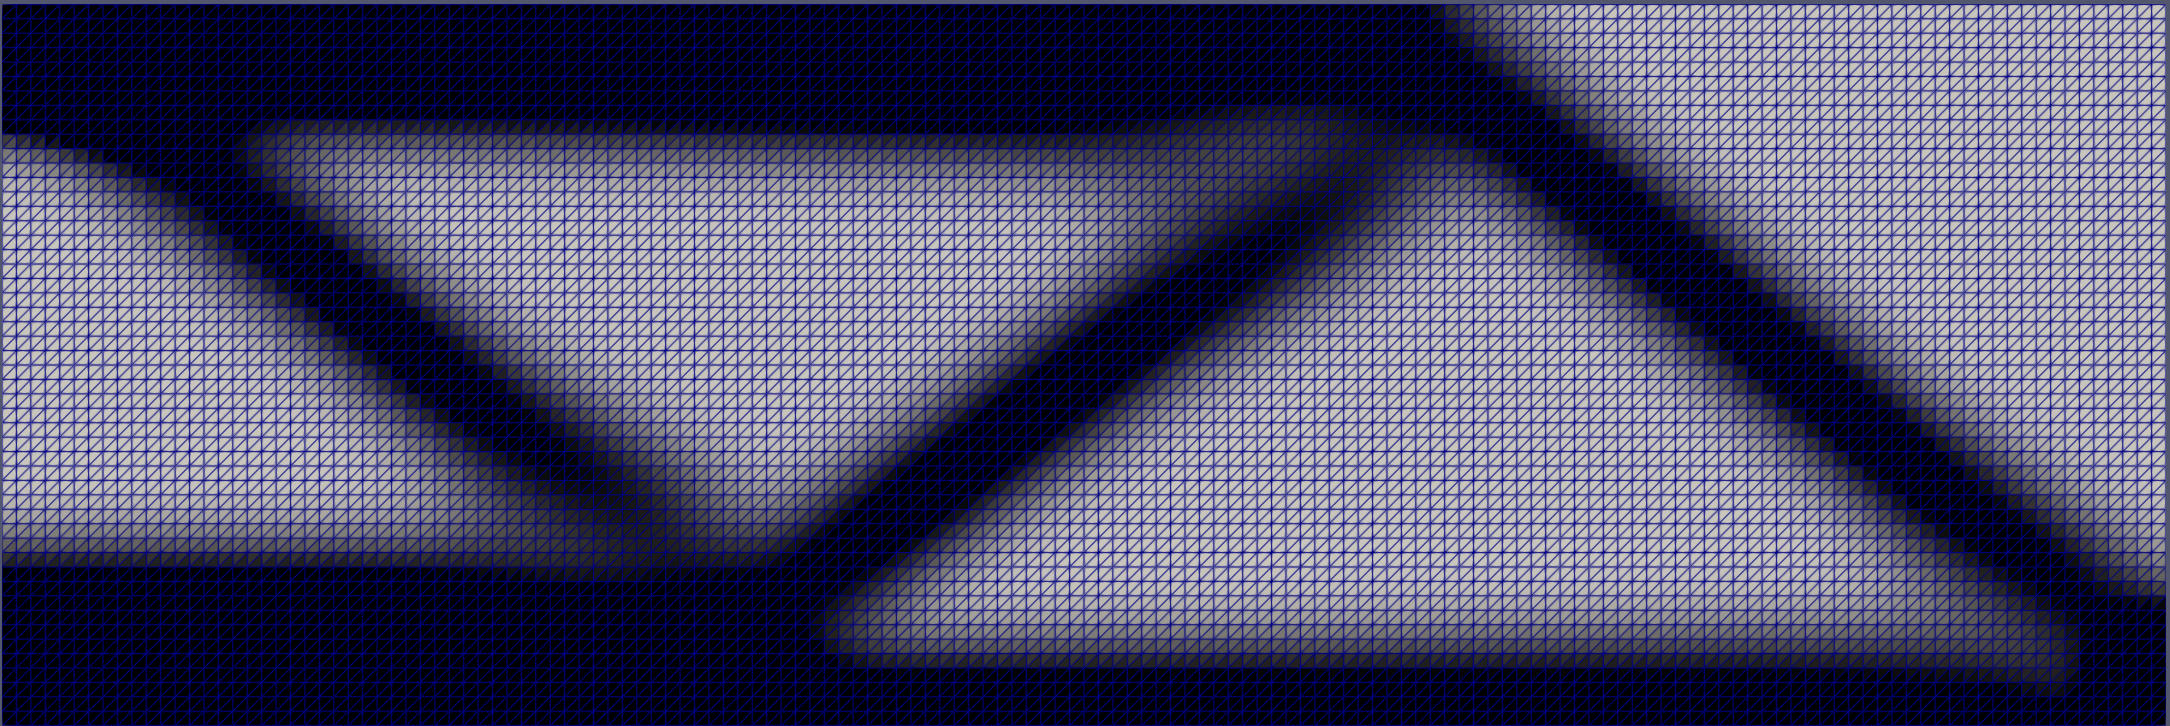
\includegraphics[width=0.5\textwidth]{figures/mbb_2d_tri.png}
		\label{fig:mbb_2d_tri}
	}
	\caption{Optimized topologies of the MBB beam using a uniform quadrilateral mesh (left) and a triangular mesh (right).}
	\label{fig:mbb_2d_all}
\end{figure}
\vspace{-2ex} % 可调节

\subsection{Different Filtering Methods}
In TO, filtering methods are essential for smoothing design variables, controlling structural details, and ensuring the quality and manufacturability of the optimized results. Thanks to its modular architecture, SOPTX allows users to seamlessly switch between different filtering strategies by simply replacing the filter class, without modifying other components of the framework.

This section compares the results of two common filters (the density filter and the Heaviside projection filter) applied to the MBB beam problem from Section~\ref{sec:exp_mbb_beam}. All parameters are kept identical except for the filter choice, with the default filter radius set to $r=6.0$.

The density filter smooths the design variables through weighted averaging, eliminating small-scale features and producing a gradual material transition. This is ideal for designs requiring structural continuity. In SOPTX, it is applied via:
\vspace{-0.5ex} % 可调节
\begin{lstlisting}[language=python]
dens_filter = DensityBasicFilter(mesh=mesh, rmin=6.0)
\end{lstlisting}
\vspace{-0.5ex} % 可调节

In contrast, the Heaviside projection filter builds on the density filter by adding a projection step. It gradually increases the projection parameter $\beta$ to drive variables toward 0 or 1, yielding a clear black-and-white topology suited for strict manufacturability. To avoid overly thick structures early on, the filter radius is reduced to $r=4.5$. It is enabled in SOPTX with:
\vspace{-0.5ex} % 可调节
\begin{lstlisting}[language=python]
heavi_filter = HeavisideProjectionBasicFilter(mesh=mesh, rmin=4.5, beta=1, max_beta=512, continuation_iter=50)   
\end{lstlisting}
\vspace{-0.5ex} % 可调节

The optimized topologies are shown in Figure~\ref{fig:mbb_filter_all}. The density filter yields a smoother design with blurred edges, while the Heaviside projection filter produces a crisp, binarized layout with lower compliance (191.4873 vs. 235.7337), indicating a stiffer structure. However, with the Heaviside projection filter, small holes may still appear due to its focus on global binarization rather than strict local control.
\vspace{-2ex} % 可调节
\begin{figure}[htp]
	\centering
	\subfloat[$c(\rho)=235.7337,~v(\rho)=0.5000$]{
		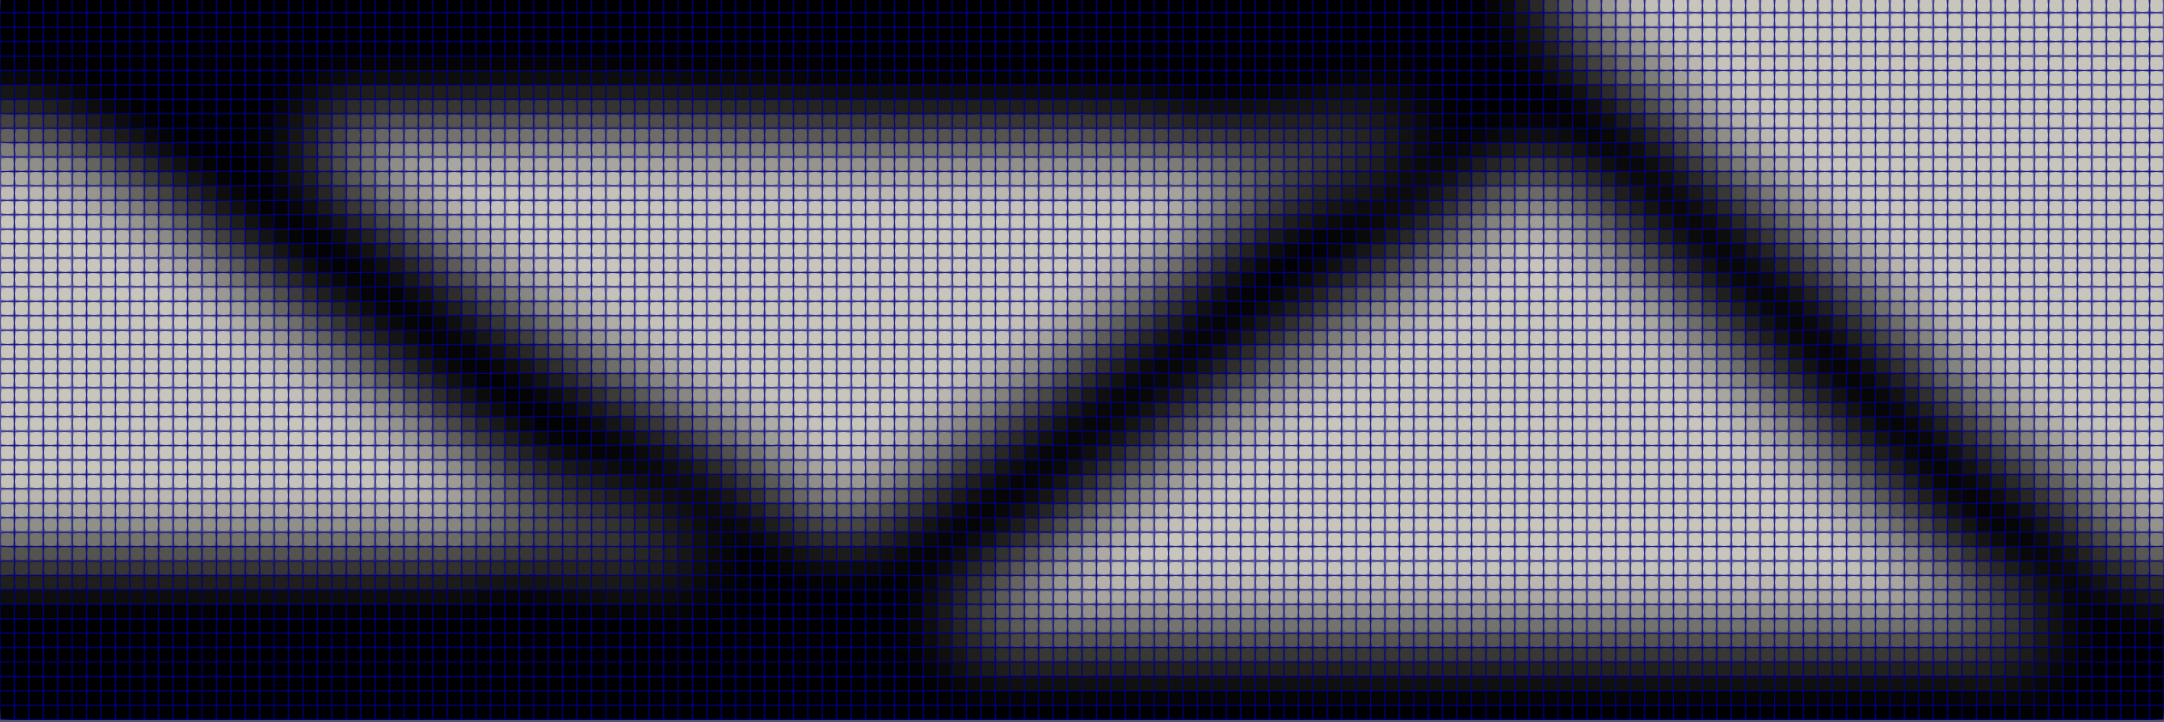
\includegraphics[width=0.5\textwidth]{figures/mbb_dens.png}
		\label{fig:mbb_dens}
	}
	\subfloat[$c(\rho)=191.4873,~v(\rho)=0.5000$]{
		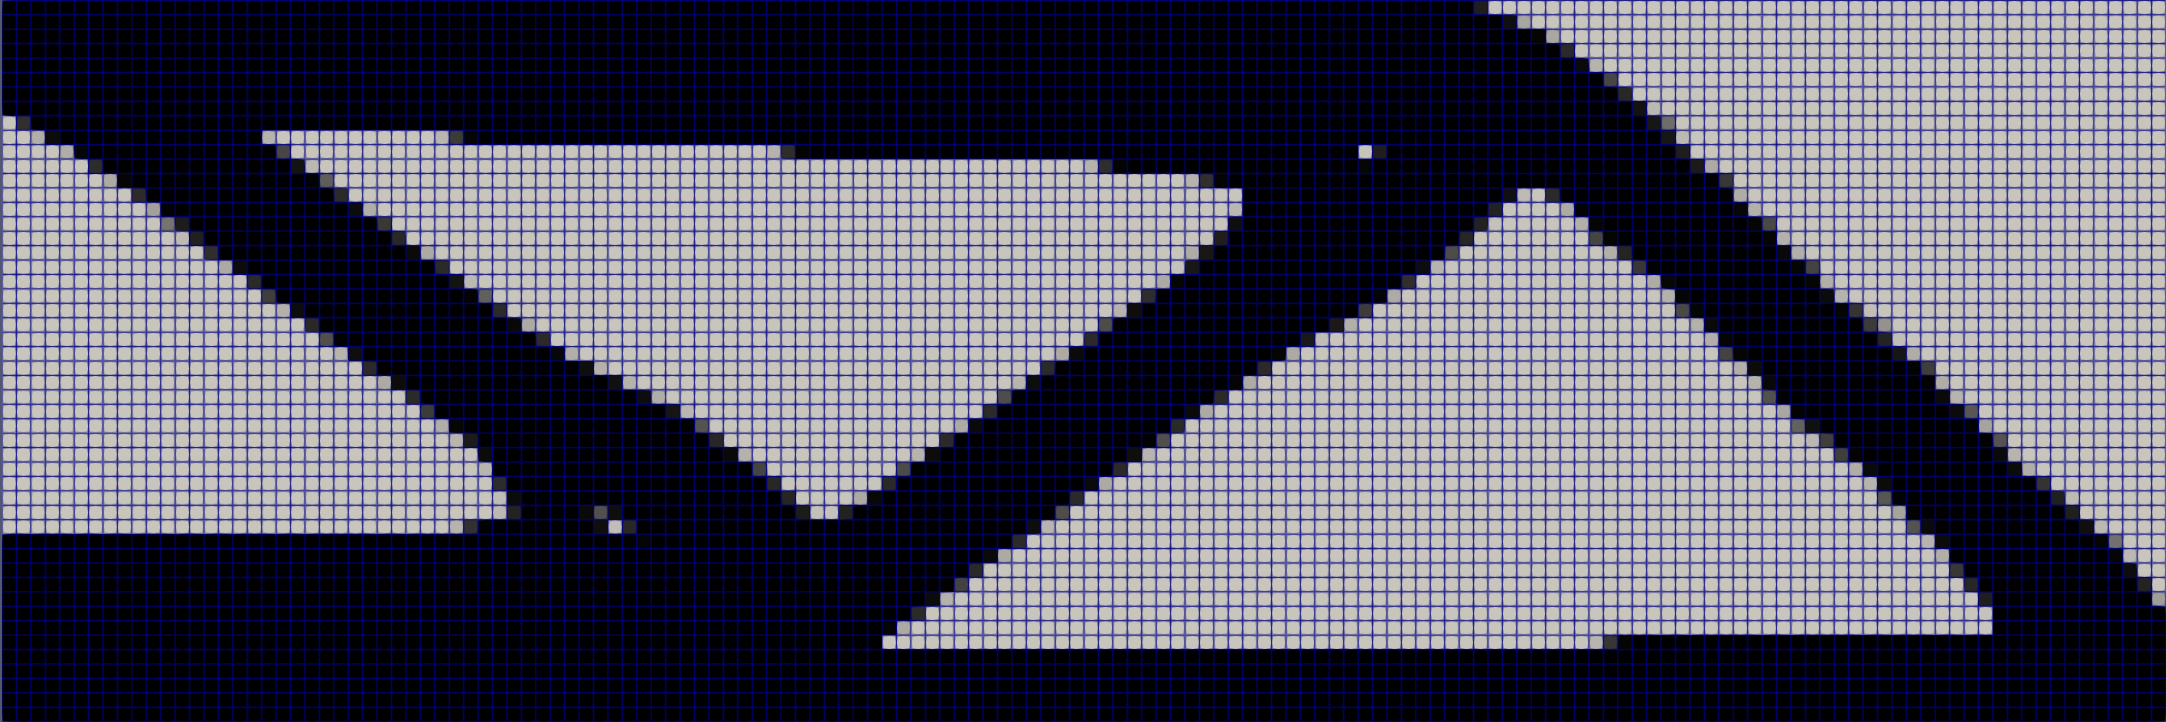
\includegraphics[width=0.5\textwidth]{figures/mbb_heavi.png}
		\label{fig:mbb_heavi}
	}
	\caption{Optimized topologies of the MBB beam using the density filter (left) and the Heaviside projection filter (right).}
	\label{fig:mbb_filter_all}
\end{figure}
\vspace{-2ex} % 可调节

In summary, SOPTX's flexibility allows efficient exploration of filter impacts on design smoothness, manufacturability, and performance.

\subsection{Different Optimization Algorithms}
In TO, the choice of optimization algorithm impacts both computational efficiency and design quality. SOPTX’s modular design allows seamless switching between optimizers, such as from the Optimality Criteria (OC) method to the more versatile Method of Moving Asymptotes (MMA). This section demonstrates this process using the MBB beam problem and highlights the refactored MMA in SOPTX.

To switch to MMA, users simply import and configure the \texttt{MMAOptimizer} class:
\vspace{-0.5ex} % 可调节
\begin{lstlisting}[language=python]
from soptx.opt import MMAOptimizer
optimizer = MMAOptimizer(objective=objective, 
		constraint=constraint, filter_=sens_filter,
		options={'max_iterations': 200, 'tolerance': 0.01})
\end{lstlisting}
\vspace{-0.5ex} % 可调节

For the MBB beam problem, MMA produces topologies nearly identical to OC’s, with compliance and volume fraction differences below $1\%$, as shown in Figure~\ref{fig:mbb_mma_all}. This consistency confirms MMA’s reliability for single-constraint problems.
\vspace{-2ex} % 可调节
\begin{figure}[htp]
	\centering
	\subfloat[$c(\rho)=219.4545,~v(\rho)=0.5000$]{
		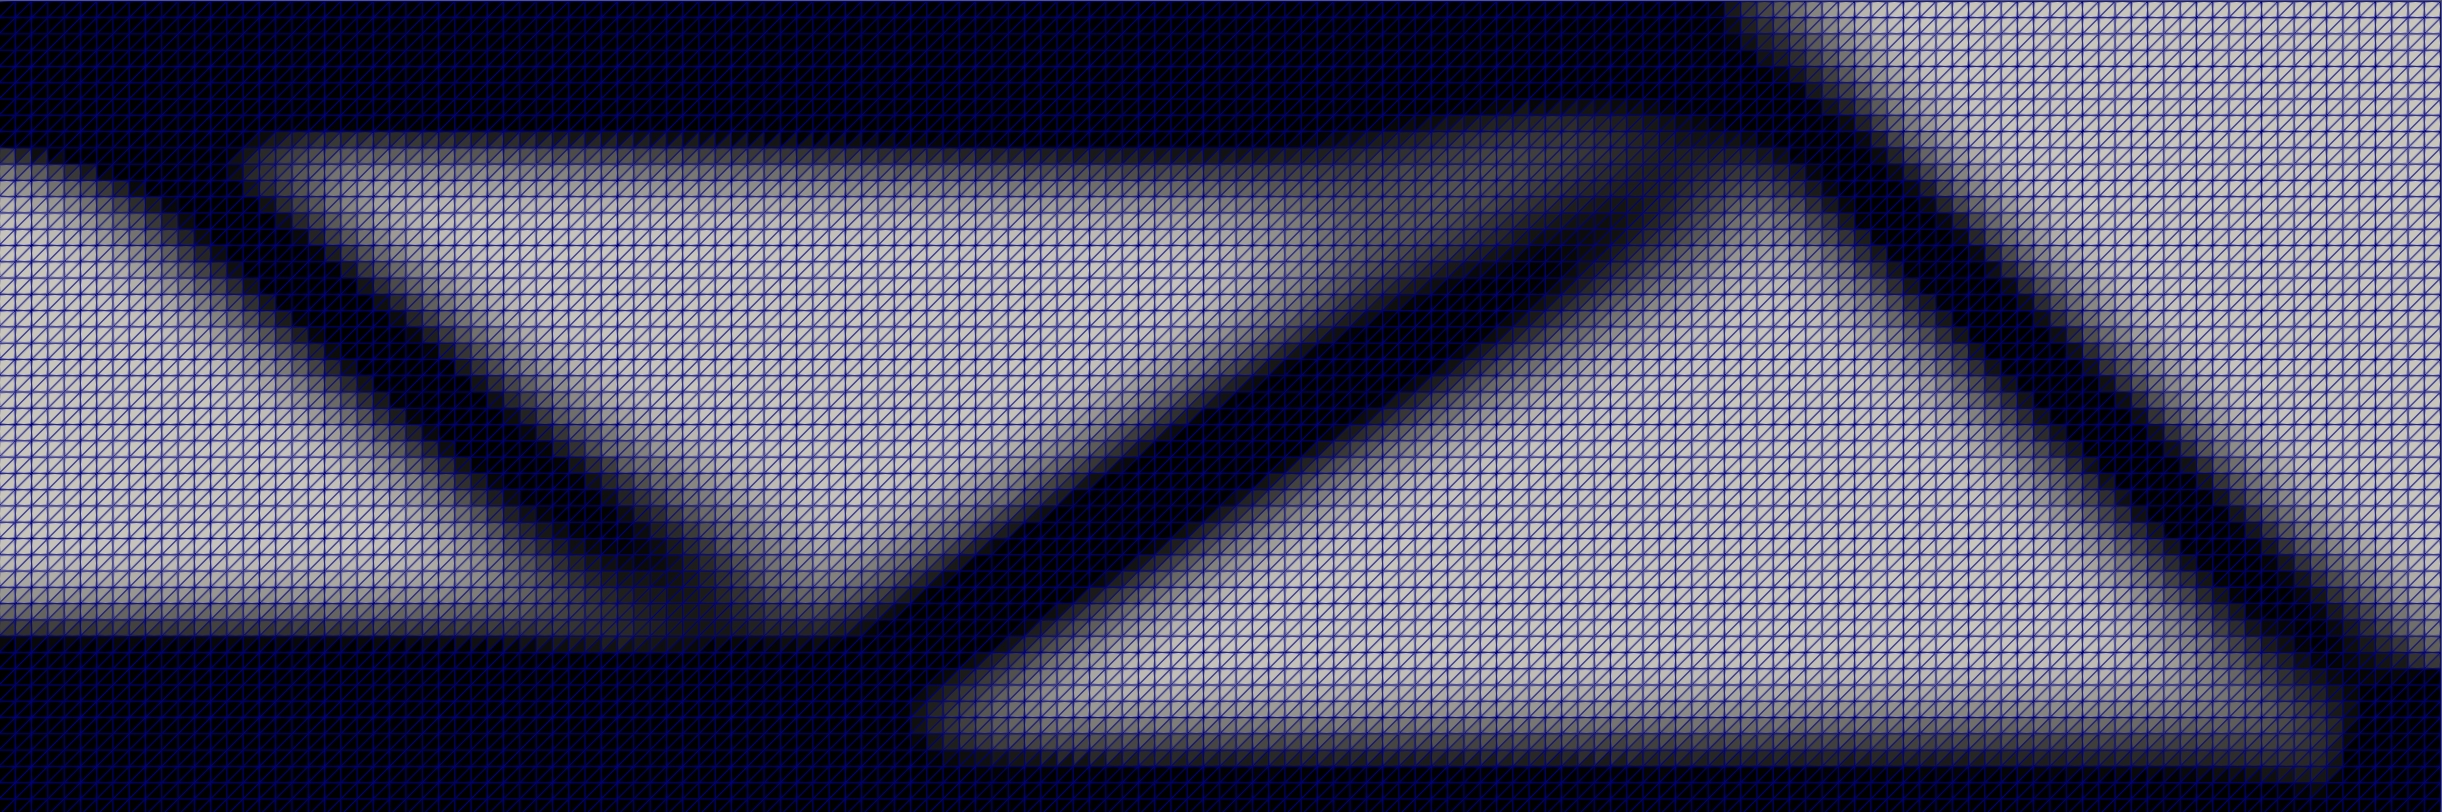
\includegraphics[width=0.5\textwidth]{figures/mbb_mma_u2.png}
		\label{fig:mbb_mma_u2}
	}
	\subfloat[$c(\rho)=220.4377,~v(\rho)=0.4995$]{
		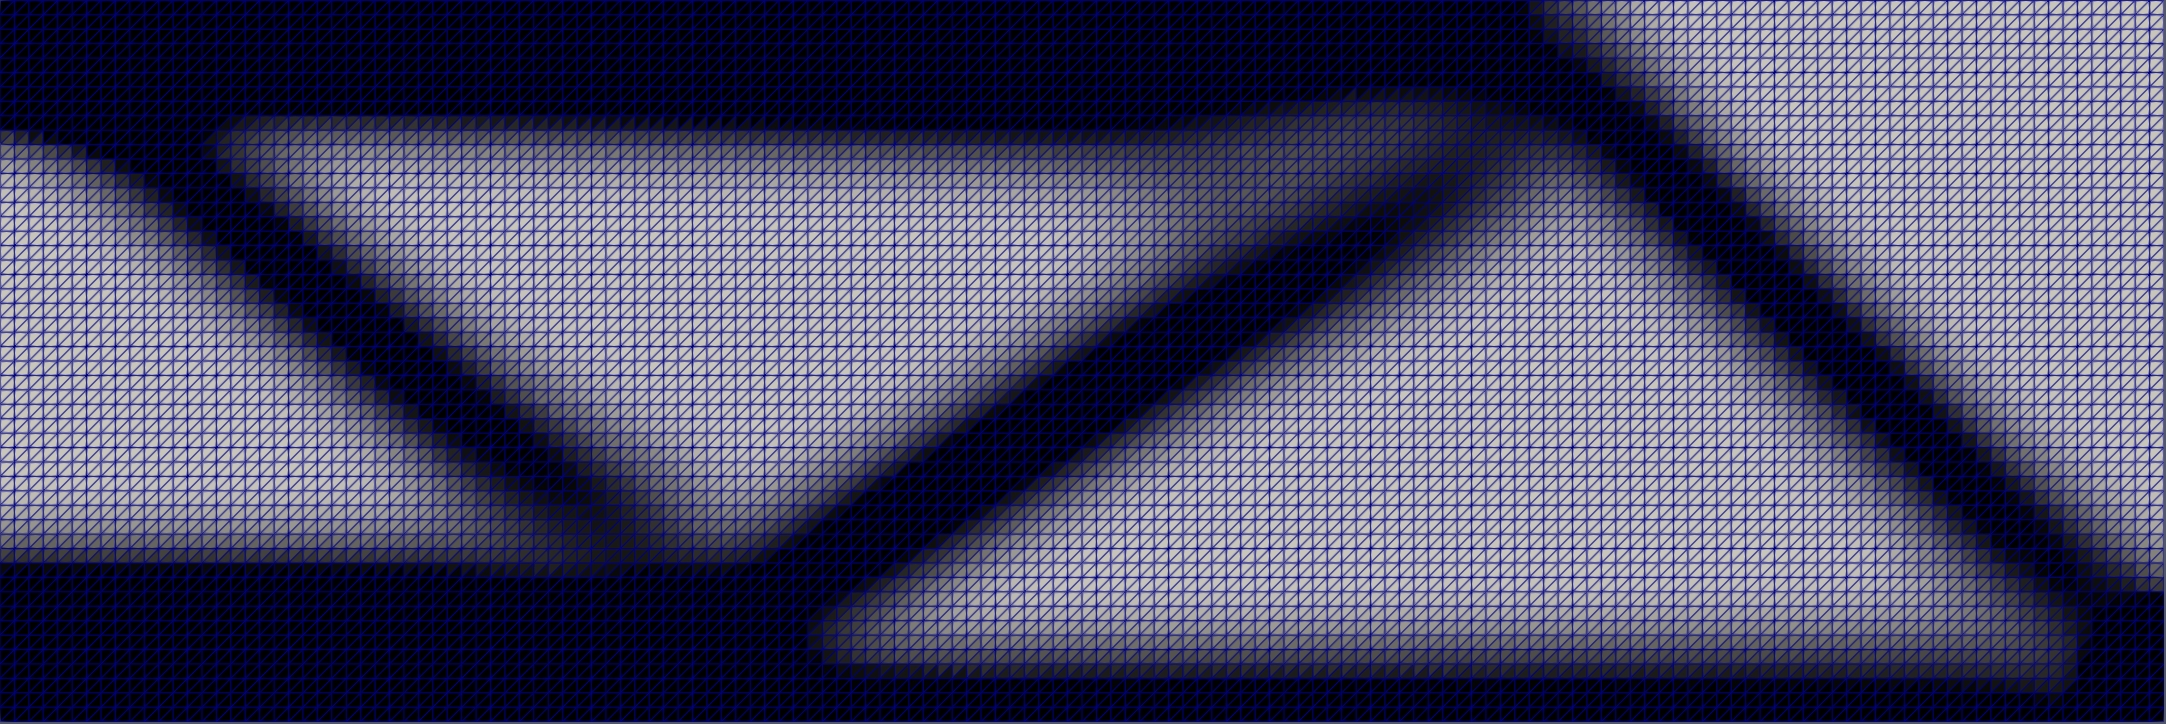
\includegraphics[width=0.5\textwidth]{figures/mbb_mma_tri.png}
		\label{fig:mbb_mma_tri}
	}
	\caption{Optimized topologies of the MBB beam using MMA optimizer on a structured quadrilateral mesh (left) and a triangular mesh (right).}
	\label{fig:mbb_mma_all}
\end{figure}
\vspace{-2ex} % 可调节

SOPTX’s MMA, refactored from Krister Svanberg’s implementation ~\cite{Svanberg2007MmaAG}, allows users to adjust internal parameters, including \texttt{m}, \texttt{n}, \texttt{xmin}, \texttt{xmax}, and control parameters like \texttt{a0}, \texttt{a}, \texttt{c}, \texttt{d}. This provides greater flexibility than traditional \textit{black-box} versions, enhancing performance and adaptability across platforms. An example configuration is shown below:
\vspace{-0.5ex} % 可调节
\begin{lstlisting}[language=python]
optimizer.options.set_advanced_options(m=1, n=NC,
			xmin=bm.zeros((NC, 1)), xmax=bm.ones((NC, 1)),
			a0=1, a=bm.zeros((1, 1)),
			c=1e4 * bm.ones((1, 1)), d=bm.zeros((1, 1)))
\end{lstlisting}
\vspace{-0.5ex} % 可调节

Through this refactoring, SOPTX not only enhances the performance of the MMA algorithm but also overcomes the limitations of conventional implementations. It provides users with greater control and cross-platform flexibility, making it particularly advantageous for both research and engineering applications in TO.

\subsection{3D Extension}\label{sec:exp_canti3d}
SOPTX’s modular design enables a smooth transition from 2D to 3D TO. This section showcases its capability with a 3D cantilever beam compliance minimization problem (see Figure~\ref{fig:cantilever_3d}). The beam is fixed on the left and bears a downward load $T=-1$ at the bottom right. A $60\times20\times4$ hexahedral mesh is applied, with a target volume fraction of 0.3, material properties $E=1$ and $\nu=0.3$, and a SIMP penalty factor $p=3$. A sensitivity filter (radius $r=1.5$) ensures smooth results.
\vspace{-2ex} % 可调节
\begin{figure}[htp]
	\centering
	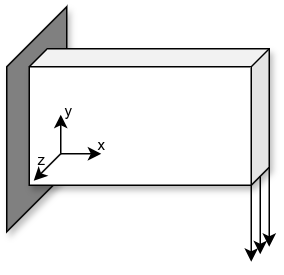
\includegraphics[width=0.5\textwidth]{figures/cantilever_3d.png}
	\caption{Geometric configuration of the 3D cantilever beam. The left end is fully fixed, and a downward concentrated load is applied at the bottom of the right end.}
	\label{fig:cantilever_3d}
\end{figure}
\vspace{-2ex} % 可调节

Compared to the 2D cantilever beam in Section~\ref{sec:exp_canti_beam}, SOPTX extends to 3D by simply replacing the PDE model and mesh configuration. The 3D cantilever beam model is implemented as follows:
\vspace{-0.5ex} % 可调节
\begin{lstlisting}[language=python]
from soptx.pde import Cantilever3dData1
pde = Cantilever3dData1(xmin=0, xmax=60, ymin=0, ymax=20, zmin=0, zmax=4, T=-1)
from fealpy.mesh import UniformMesh3d
mesh = UniformMesh3d(extent=[0, 60, 0, 20, 0, 4], h=[1, 1, 1], origin=[0, 0, 0])
\end{lstlisting}
\vspace{-0.5ex} % 可调节
The complete definition of the \texttt{Cantilever3dData1} model is available in Appendix~\ref{sec:code_canti_3d}.

The initial material density is uniformly set to the target volume fraction of 0.3. Using the OC optimizer and a sensitivity filter with radius $r=1.5$, the compliance $c(\rho)$ shows a rapid initial decrease, followed by a gradual convergence with slight fluctuations, stabilizing at around 2,000 by iteration 54 (see Figure~\ref{fig:canti_3d_convergence}). The volume fraction remains nearly constant around 0.3 throughout the process, indicating effective constraint control.
\vspace{-2ex} % 可调节
\begin{figure}[htp]
	\centering
	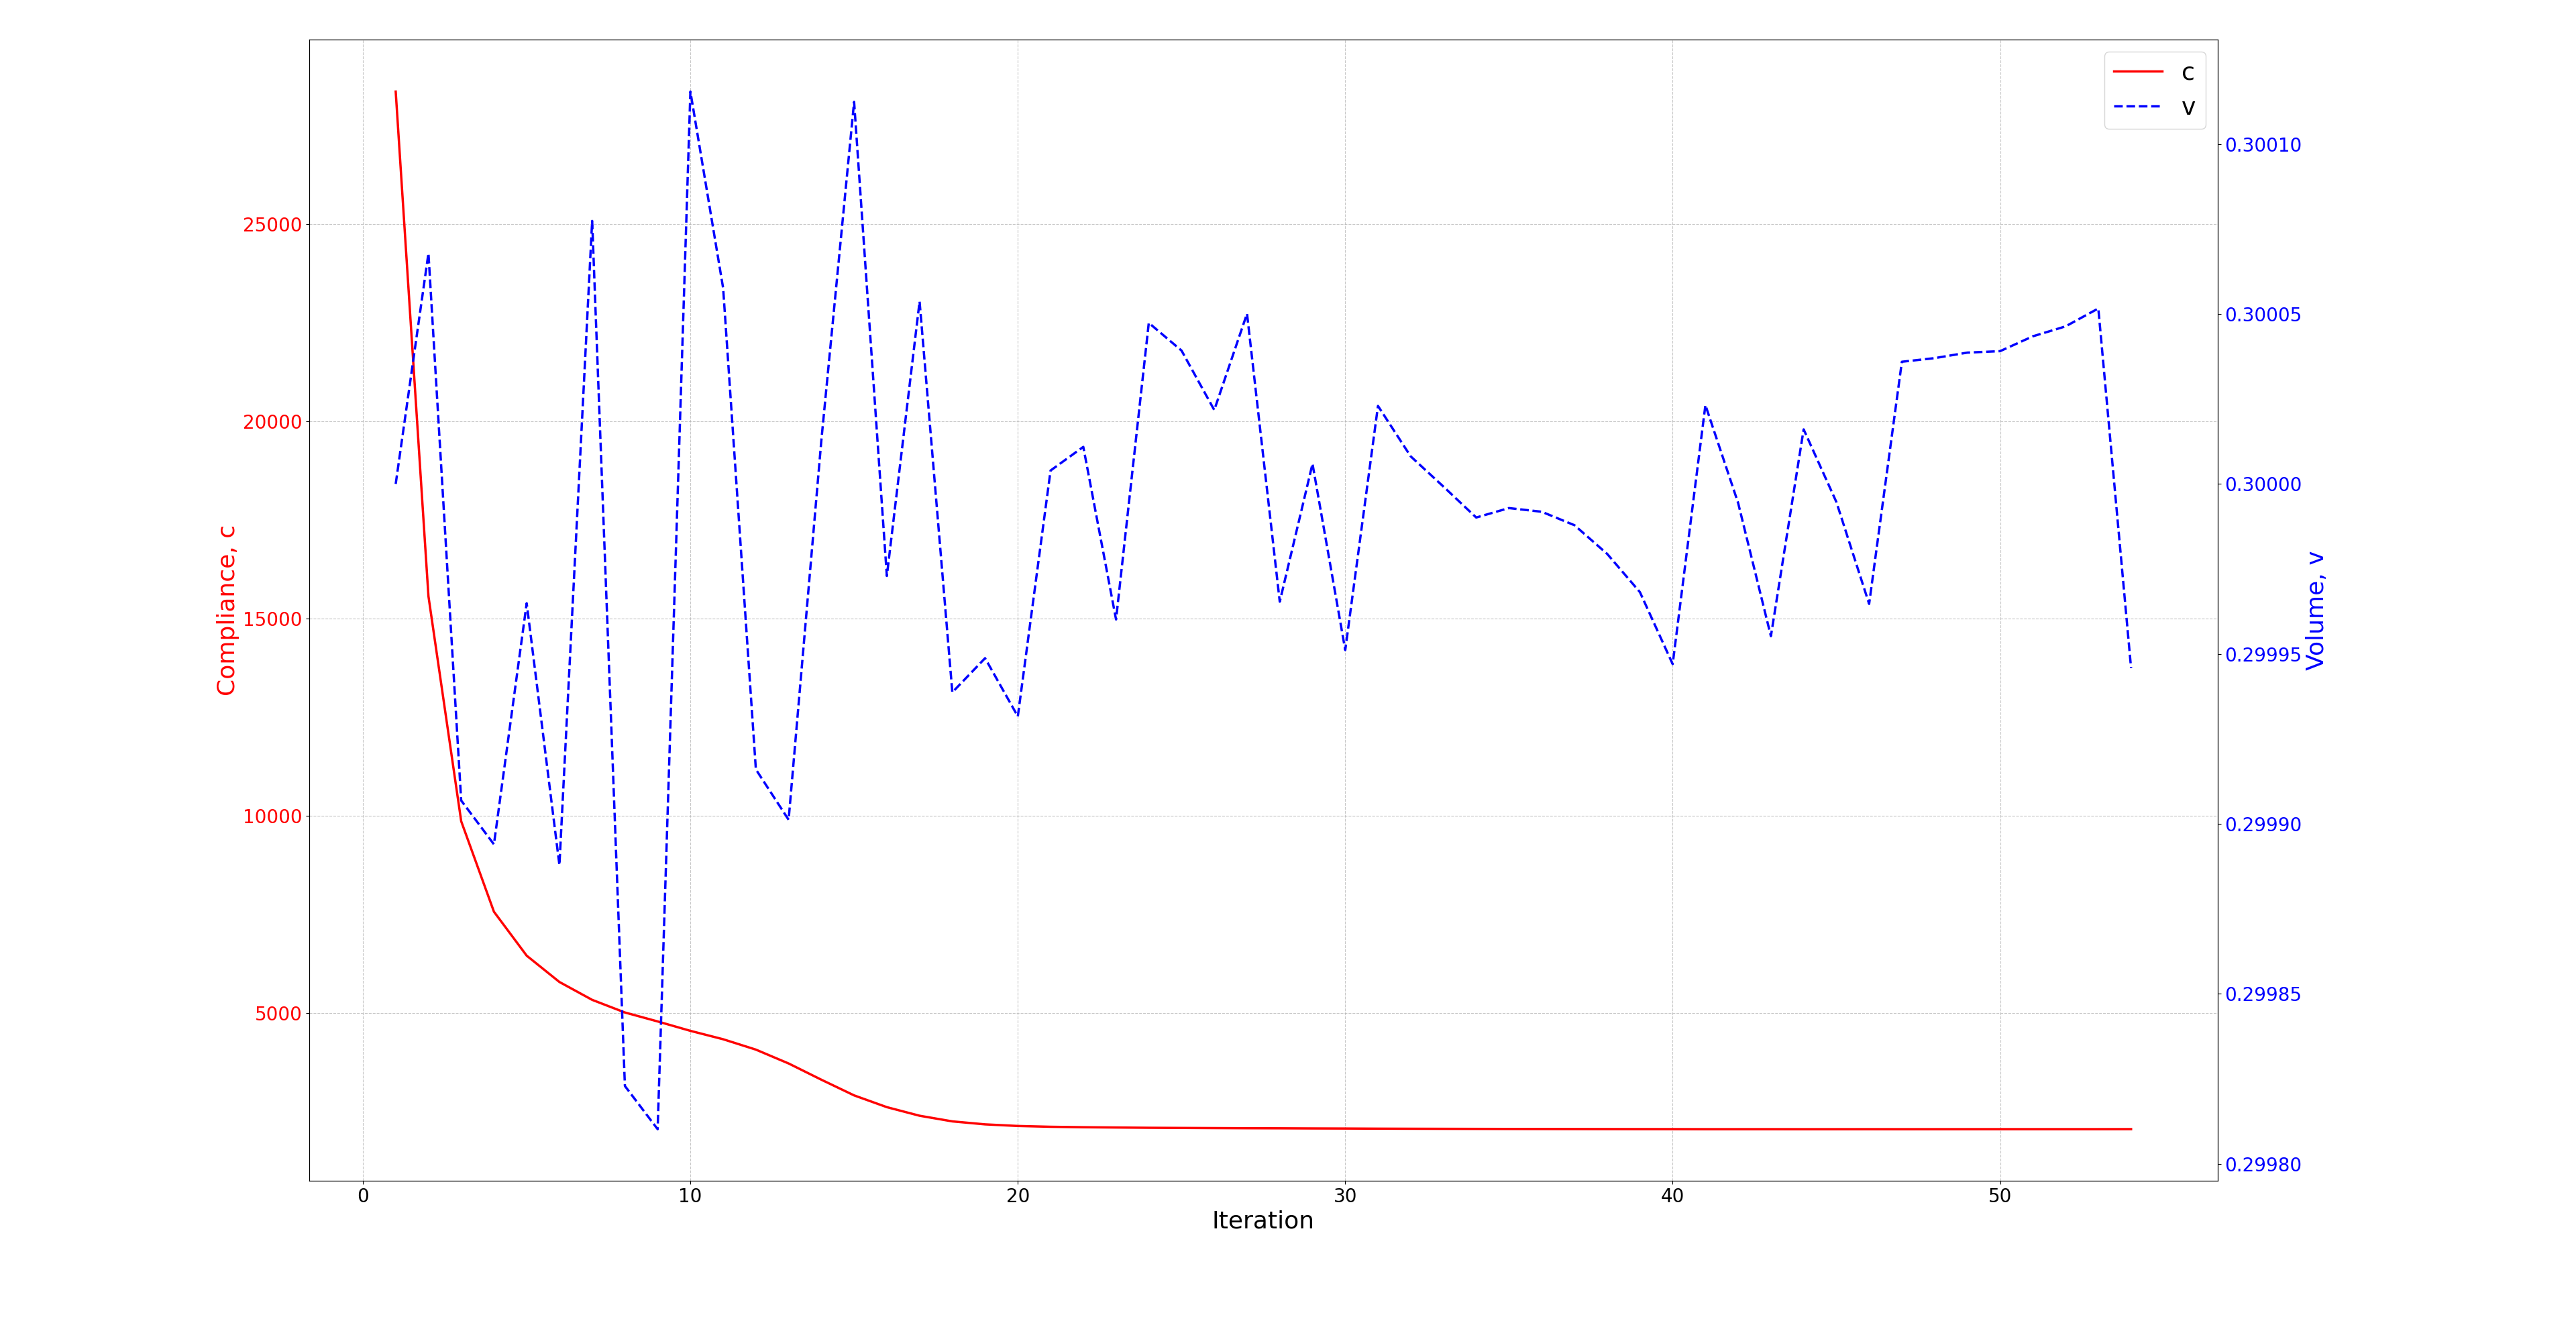
\includegraphics[width=0.85\textwidth]{figures/cantilever_3d_convergence.png}
	\caption{Convergence histories of the compliance $c(\rho)$ and volume fraction $v(\rho)$ for the 3D cantilever beam initialized with a uniform density of 0.3.}
	\label{fig:canti_3d_convergence}
\end{figure}
\vspace{-2ex} % 可调节

To better visualize the optimization results, Figure~\ref{fig:canti3d_all} shows the topology layouts at iterations 7, 21, and 54. Only elements with density values $\rho>0.3$ are rendered to highlight the structural features.
\vspace{-2ex} % 可调节
\begin{figure}[htp]
	\centering
	\subfloat[$c(\rho)=5338.9462,~v(\rho)=0.3001$]{
		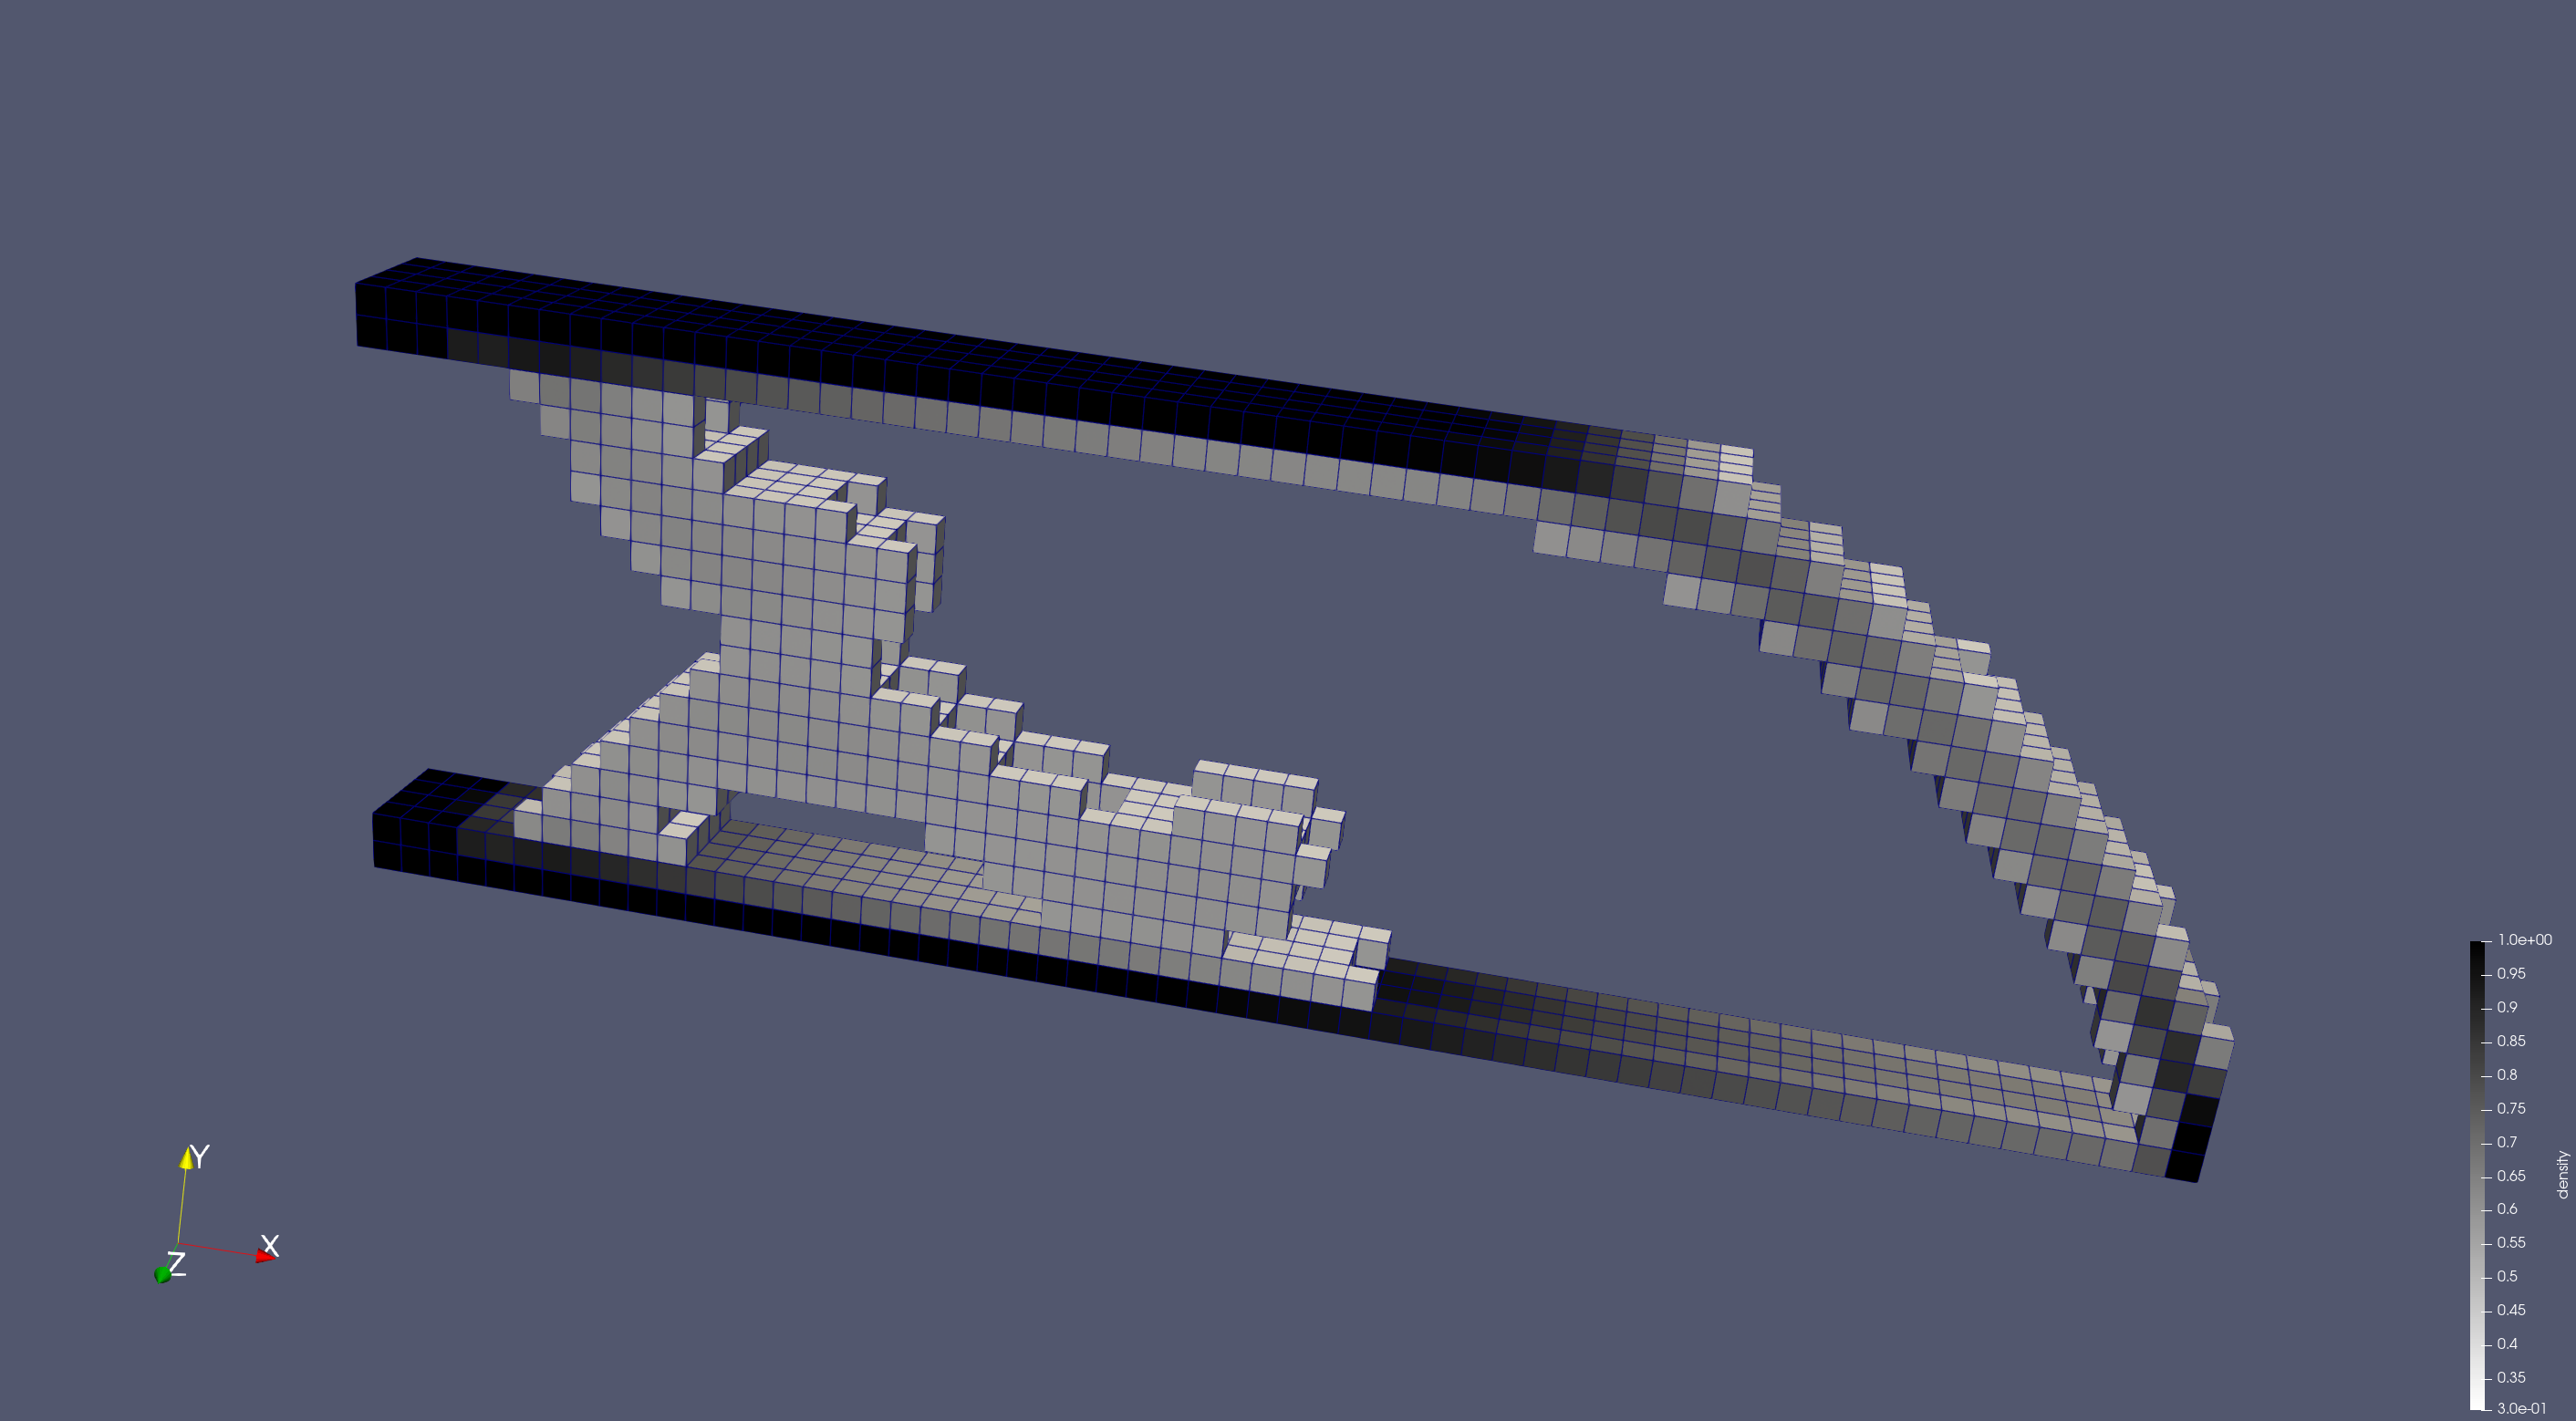
\includegraphics[width=0.32\textwidth]{figures/cantilever_3d_1.png}
		\label{fig:canti3d_1}
	}
	\subfloat[$c(\rho)=2122.6707,~v(\rho)=0.3000$]{
		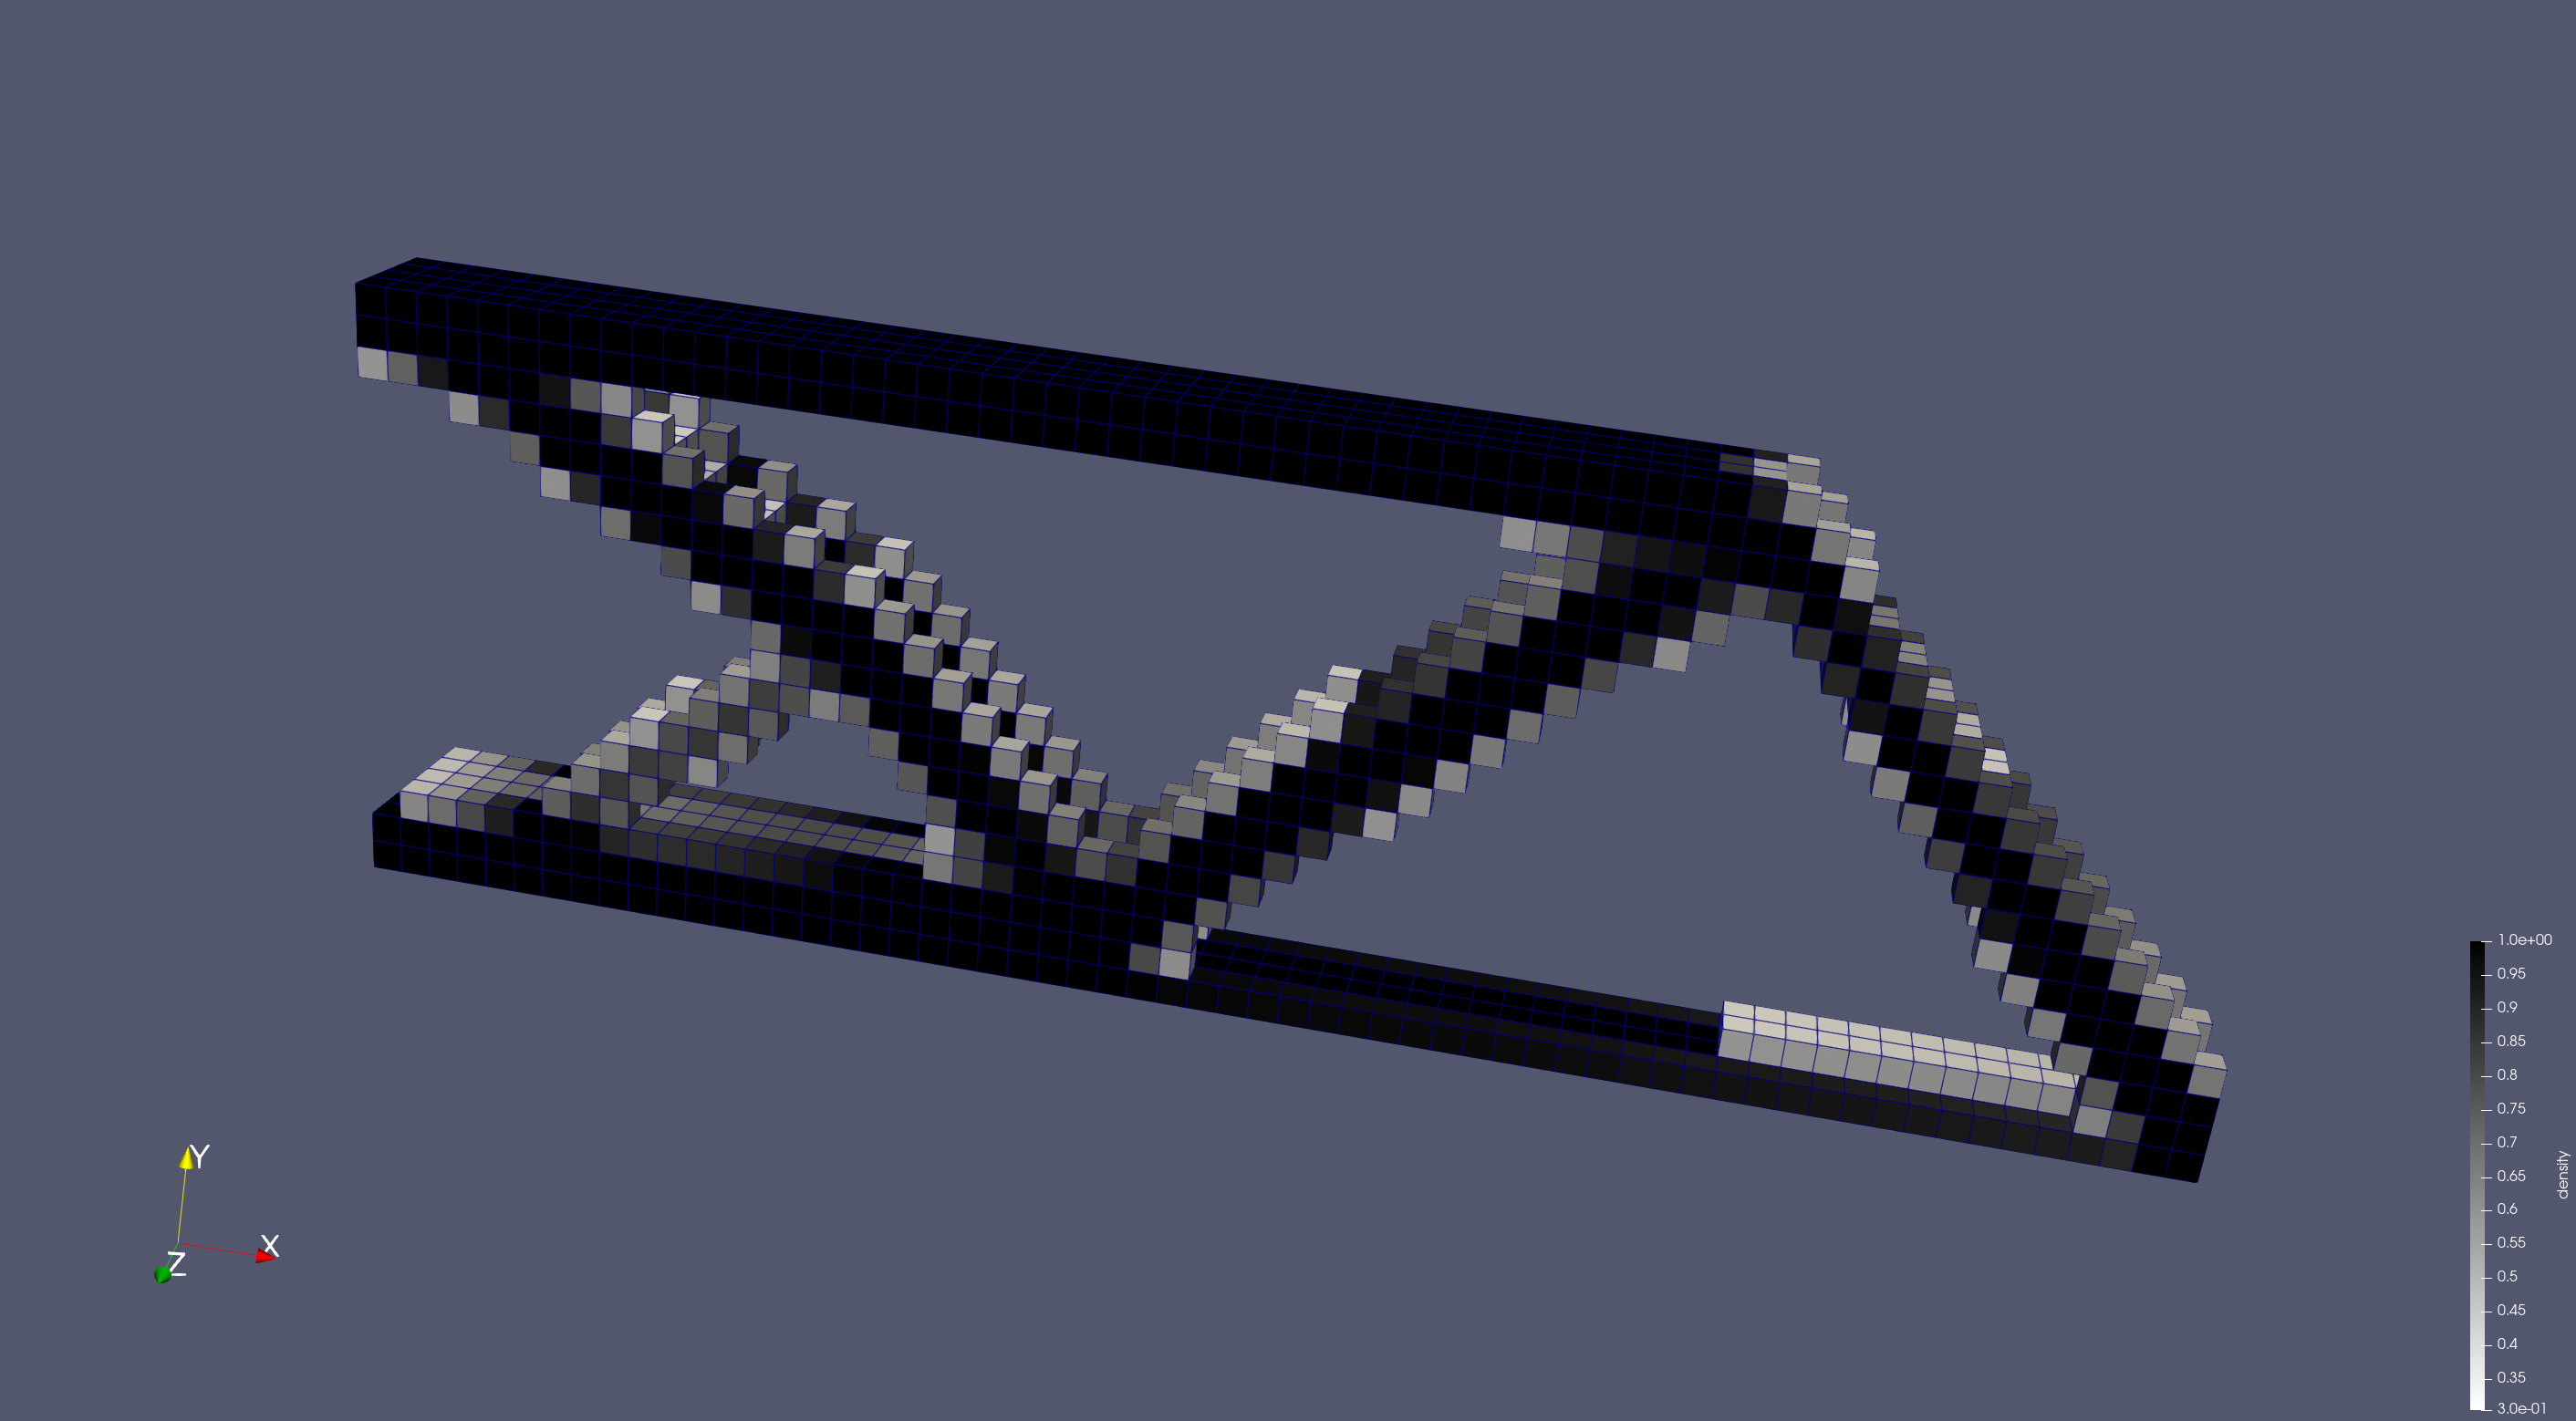
\includegraphics[width=0.32\textwidth]{figures/cantilever_3d_2.png}
		\label{fig:canti3d_2}
	}
	\subfloat[$c(\rho)=2063.5625,~v(\rho)=0.2999$]{
		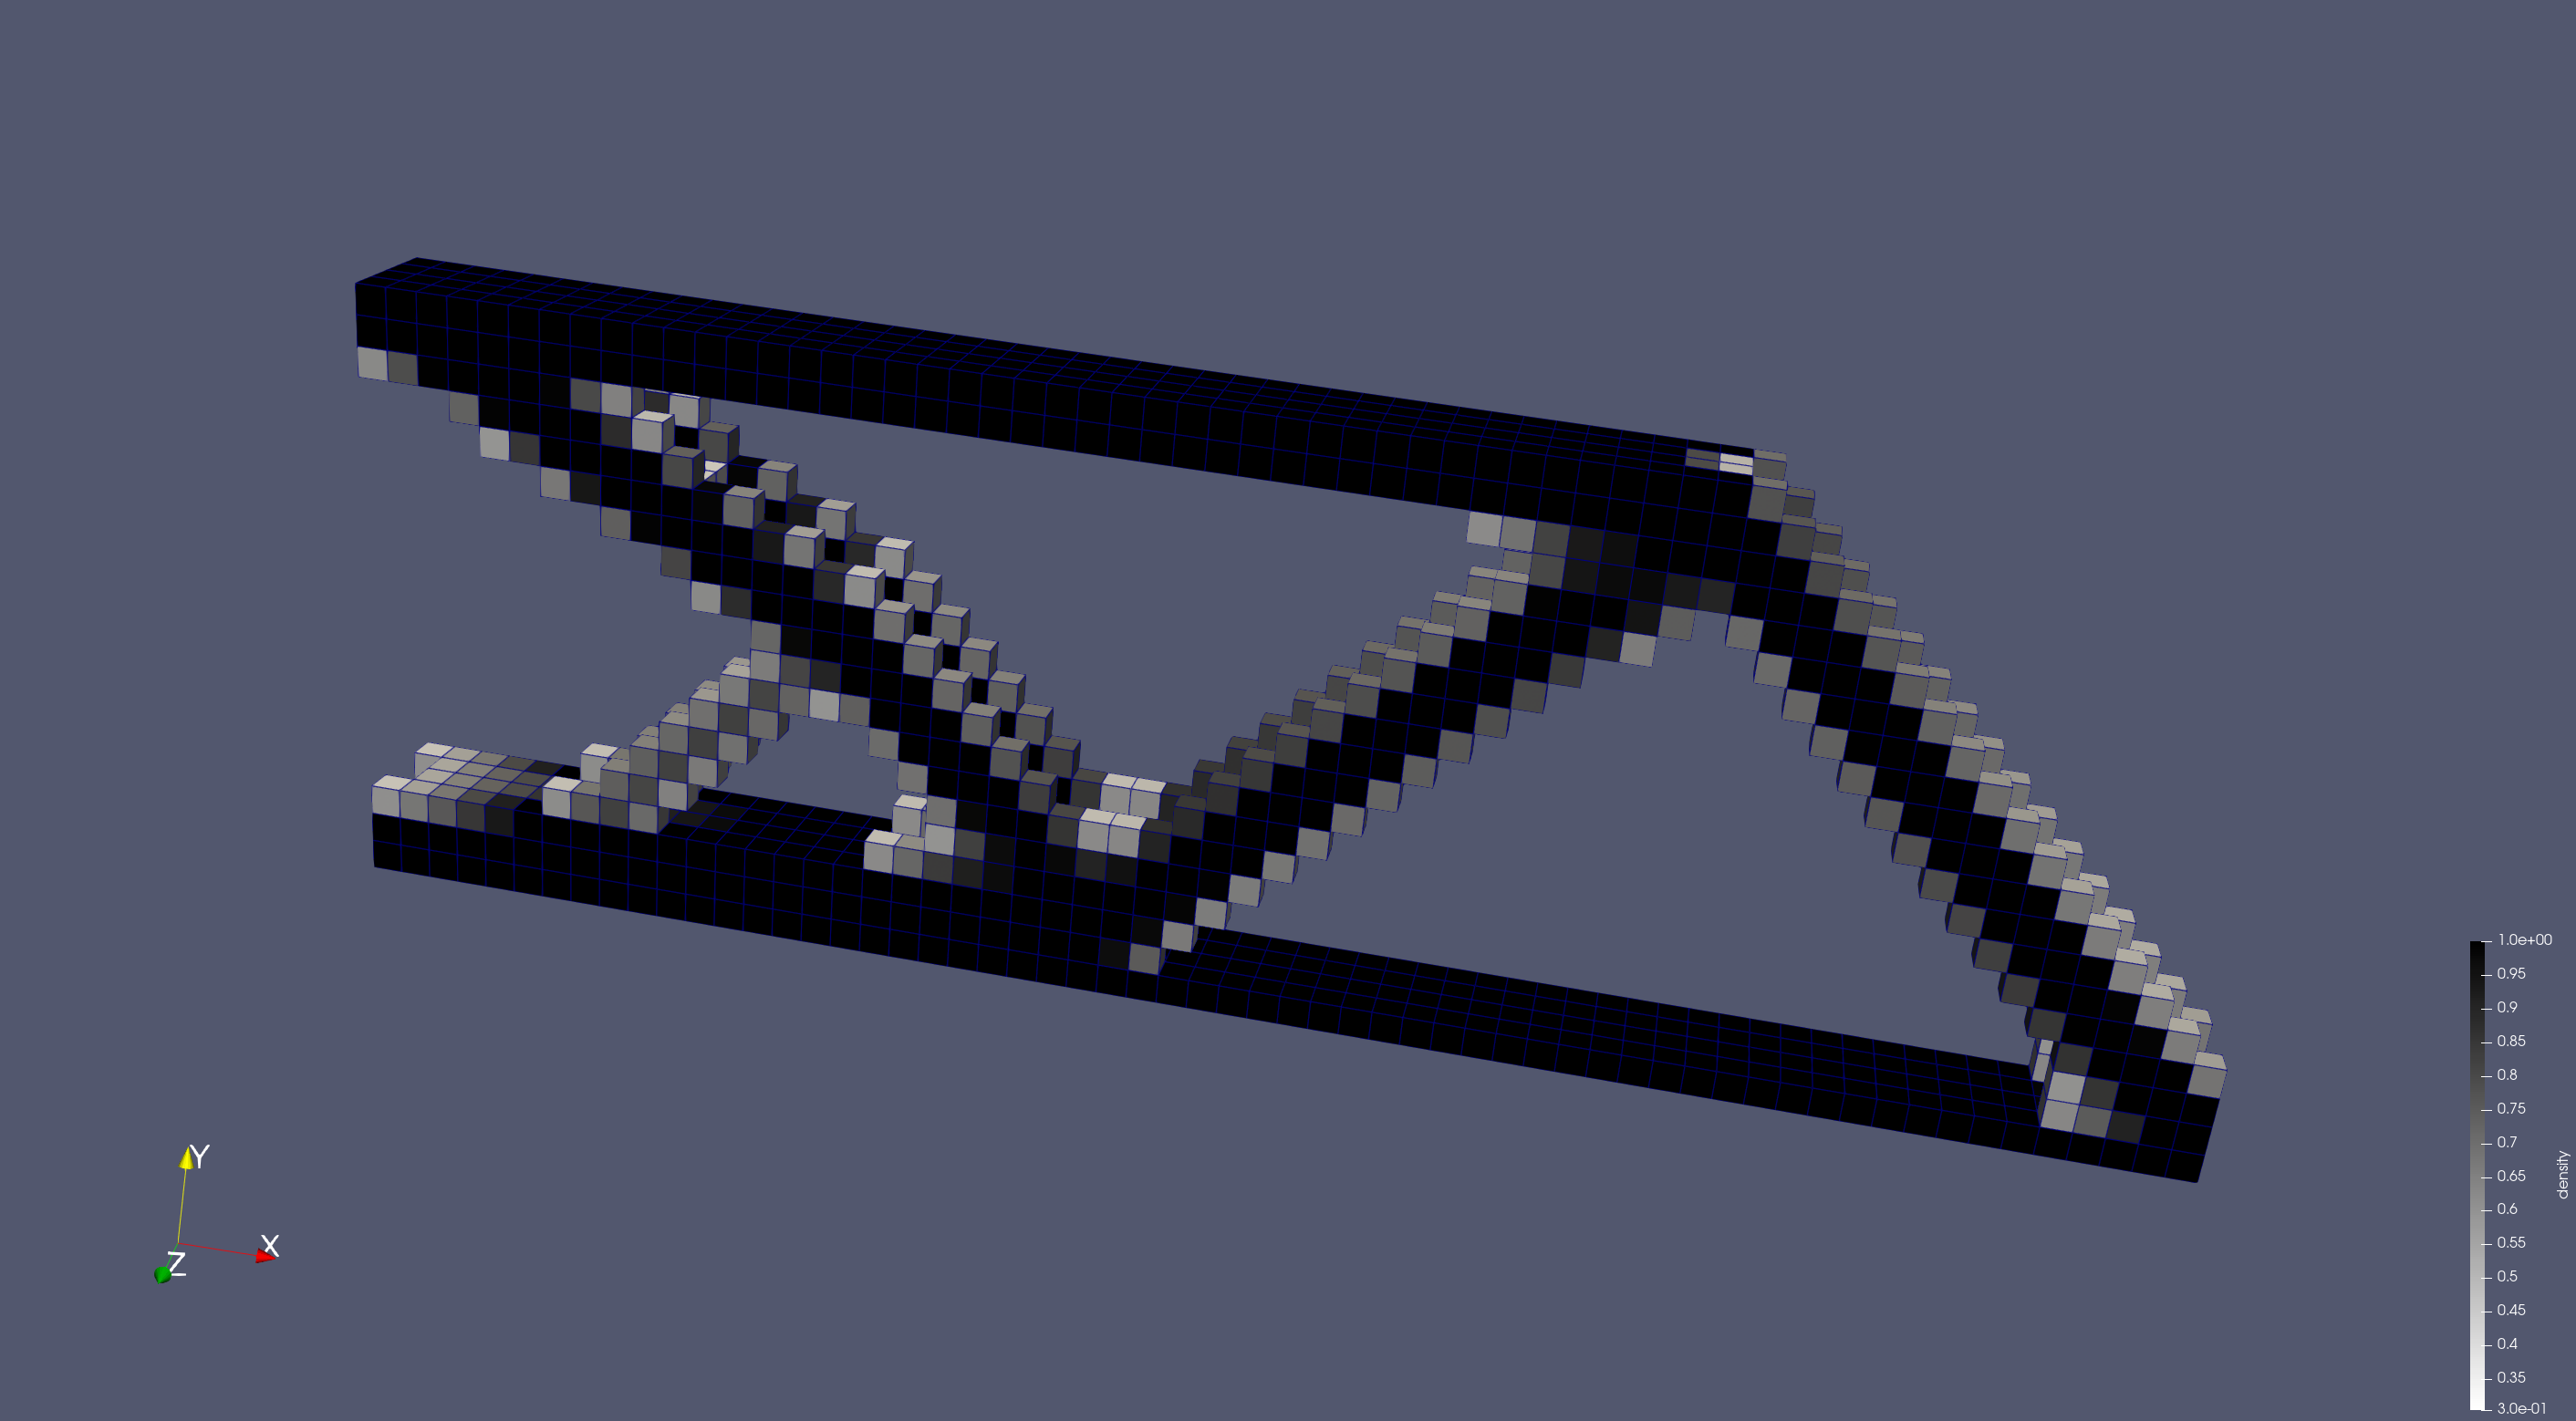
\includegraphics[width=0.32\textwidth]{figures/cantilever_3d_3.png}
		\label{fig:canti3d_3}
	}
	\caption{Topology layouts at iterations 7, 21, and 54 during the optimization of the 3D cantilever beam. Elements with $\rho > 0.3$ are visualized. Each subfigure also reports the compliance and volume fraction.}
	\label{fig:canti3d_all}
\end{figure}
\vspace{-2ex} % 可调节

3D TO increases computational complexity significantly. SOPTX addresses this with efficient matrix assembly and multi-backend support, enhancing performance for large-scale problems. Details follow in subsequent sections

\subsection{Application of Fast Matrix Assembly}
In 3D TO problems, computational efficiency is critical. For the 3D cantilever beam example (Section~\ref{sec:exp_canti3d}), the mesh of $60\times20\times4$ elements leads to 19,215 displacement degrees of freedom and 4,800 density variables, requiring 54 iterations. Traditional matrix assembly in finite element methods involves redundant computations, creating a bottleneck.

SOPTX addresses this with a fast matrix assembly technique that separates element-dependent and element-independent parts, reusing invariant quantities to accelerate the process. Additionally, symbolic integration precomputation analytically integrates invariant terms in advance, improving accuracy and stability.
\vspace{-0.5ex} % 可调节
\begin{itemize} 
	\item \textbf{Fast assembly}: Accelerates matrix assembly by separating element-dependent and element-independent terms, coupled with efficient numerical integration.
	\item \textbf{Symbolic Fast Assembly}: Further improves accuracy and stability by analytically integrating invariant terms ahead of time.
\end{itemize}
\vspace{-0.5ex} % 可调节

Users can easily switch between assembly methods by setting the \texttt{assembly\_method} parameter in the solver initialization, as shown below:
\vspace{-0.5ex} % 可调节
\begin{lstlisting}[language=python]
# Fast Assembly
solver = ElasticFEMSolver(..., assembly_method=AssemblyMethod.FAST, ...)
# Symbolic Fast Assembly
solver = ElasticFEMSolver(..., assembly_method=AssemblyMethod.SYMBOLIC, ...)
\end{lstlisting}
\vspace{-0.5ex} % 可调节

Moreover, SOPTX employs intelligent caching to store invariant data across iterations, significantly reducing computational time in later iterations.

Table~\ref{tab:assembly_comparison} compares the performance of different matrix assembly techniques for the 3D cantilever beam optimization (Section~\ref{sec:exp_canti3d}).

\vspace{-0.5ex} % 可调节
\begin{table}[htbp]
	\centering
%	\setlength{\tabcolsep}{4pt} % 减小列间距
	\caption{Performance comparison of matrix assembly techniques in the 3D cantilever beam optimization problem. All values are reported in seconds.}
%	\small % 使用小字体
	\begin{tabular}{cccccc}
		\toprule
		\textbf{Assembly Technique} & \textbf{Total} & \textbf{1st Iter.} & \textbf{1st Assembly} & \textbf{Avg. Iter.} & \textbf{Avg. Assembly} \\
		\midrule
		Original Assembly & 68.605 & 3.342 & 1.197 & 1.231 & 0.838 \\
		Fast Assembly & 39.826 & 2.387 & 0.342 & 0.706 & 0.276 \\
		Symbolic Fast Assembly & 41.194 & 5.877 & 3.853 & 0.666 & 0.272 \\
		\bottomrule
	\end{tabular}
	\label{tab:assembly_comparison}
\end{table}
\vspace{-0.5ex} % 可调节

As shown in Table~\ref{tab:assembly_comparison}, the original assembly method has an average assembly time of \SI{0.838}{s} per iteration ($68\%$ of total iteration time), creating a bottleneck. Fast assembly reduces this to \SI{0.276}{s} ($33\%$ of the original), while symbolic integration precomputation, despite a longer first iteration (\SI{3.853}{s}), achieves the fastest average assembly time (\SI{0.272}{s}) with enhanced accuracy.

In summary, SOPTX's fast assembly strategies significantly reduce computational cost and improve accuracy, making it ideal for large-scale TO problems.

\subsection{Application of Automatic Differentiation}\label{sec:exp_canti3d_ad}
Sensitivity analysis is vital in TO to update design variables. Traditional methods rely on manual sensitivity derivation, which is time-consuming and error-prone, especially for complex models. The SOPTX framework introduces AD to streamline this process, enabling users to prioritize problem modeling over mathematical derivations. Here, we demonstrate AD’s application using the 3D cantilever beam example from Section~\ref{sec:exp_canti3d}.

The SOPTX framework supports multiple computational backends(e.g., NumPy, PyTorch, JAX). To enable AD, users must switch from the default NumPy backend to an AD-enabled backend like PyTorch~\cite{paszke2017automatic} with a single line of code:
\vspace{-0.5ex} % 可调节
\begin{lstlisting}[language=python]
bm.set_backend('pytorch')
\end{lstlisting}
\vspace{-0.5ex} % 可调节

Sensitivity computation is controlled via the \texttt{diff\_mode} parameter: \texttt{'manual'} for hand-derived formulas and \texttt{'auto'} for AD. For example, AD can be enabled for the compliance objective while keeping manual differentiation for the volume constraint:
\vspace{-0.5ex} % 可调节
\begin{lstlisting}[language=python]
obj_config = ComplianceConfig(diff_mode='auto')
objective = ComplianceObjective(solver=solver, config=obj_config)
cons_config = VolumeConfig(diff_mode='manual')
constraint = VolumeConstraint(solver=solver, volume_fraction=0.5, config=cons_config)
\end{lstlisting}
\vspace{-0.5ex} % 可调节
This setup allows selective use of AD or manual differentiation. Further details on AD implementation are in Section~\ref{sec:ad_compliance}.

To verify the correctness and effectiveness of AD, we conduct tests using the 3D cantilever beam problem described in Section~\ref{sec:exp_canti3d}. All parameters are kept identical. The structural compliance sensitivity is computed using AD. Figure~\ref{fig:canti3d_ad_convergence} shows the convergence histories of the compliance and volume fraction.
\vspace{-2ex} % 可调节
\begin{figure}[htp] 
	\centering 
	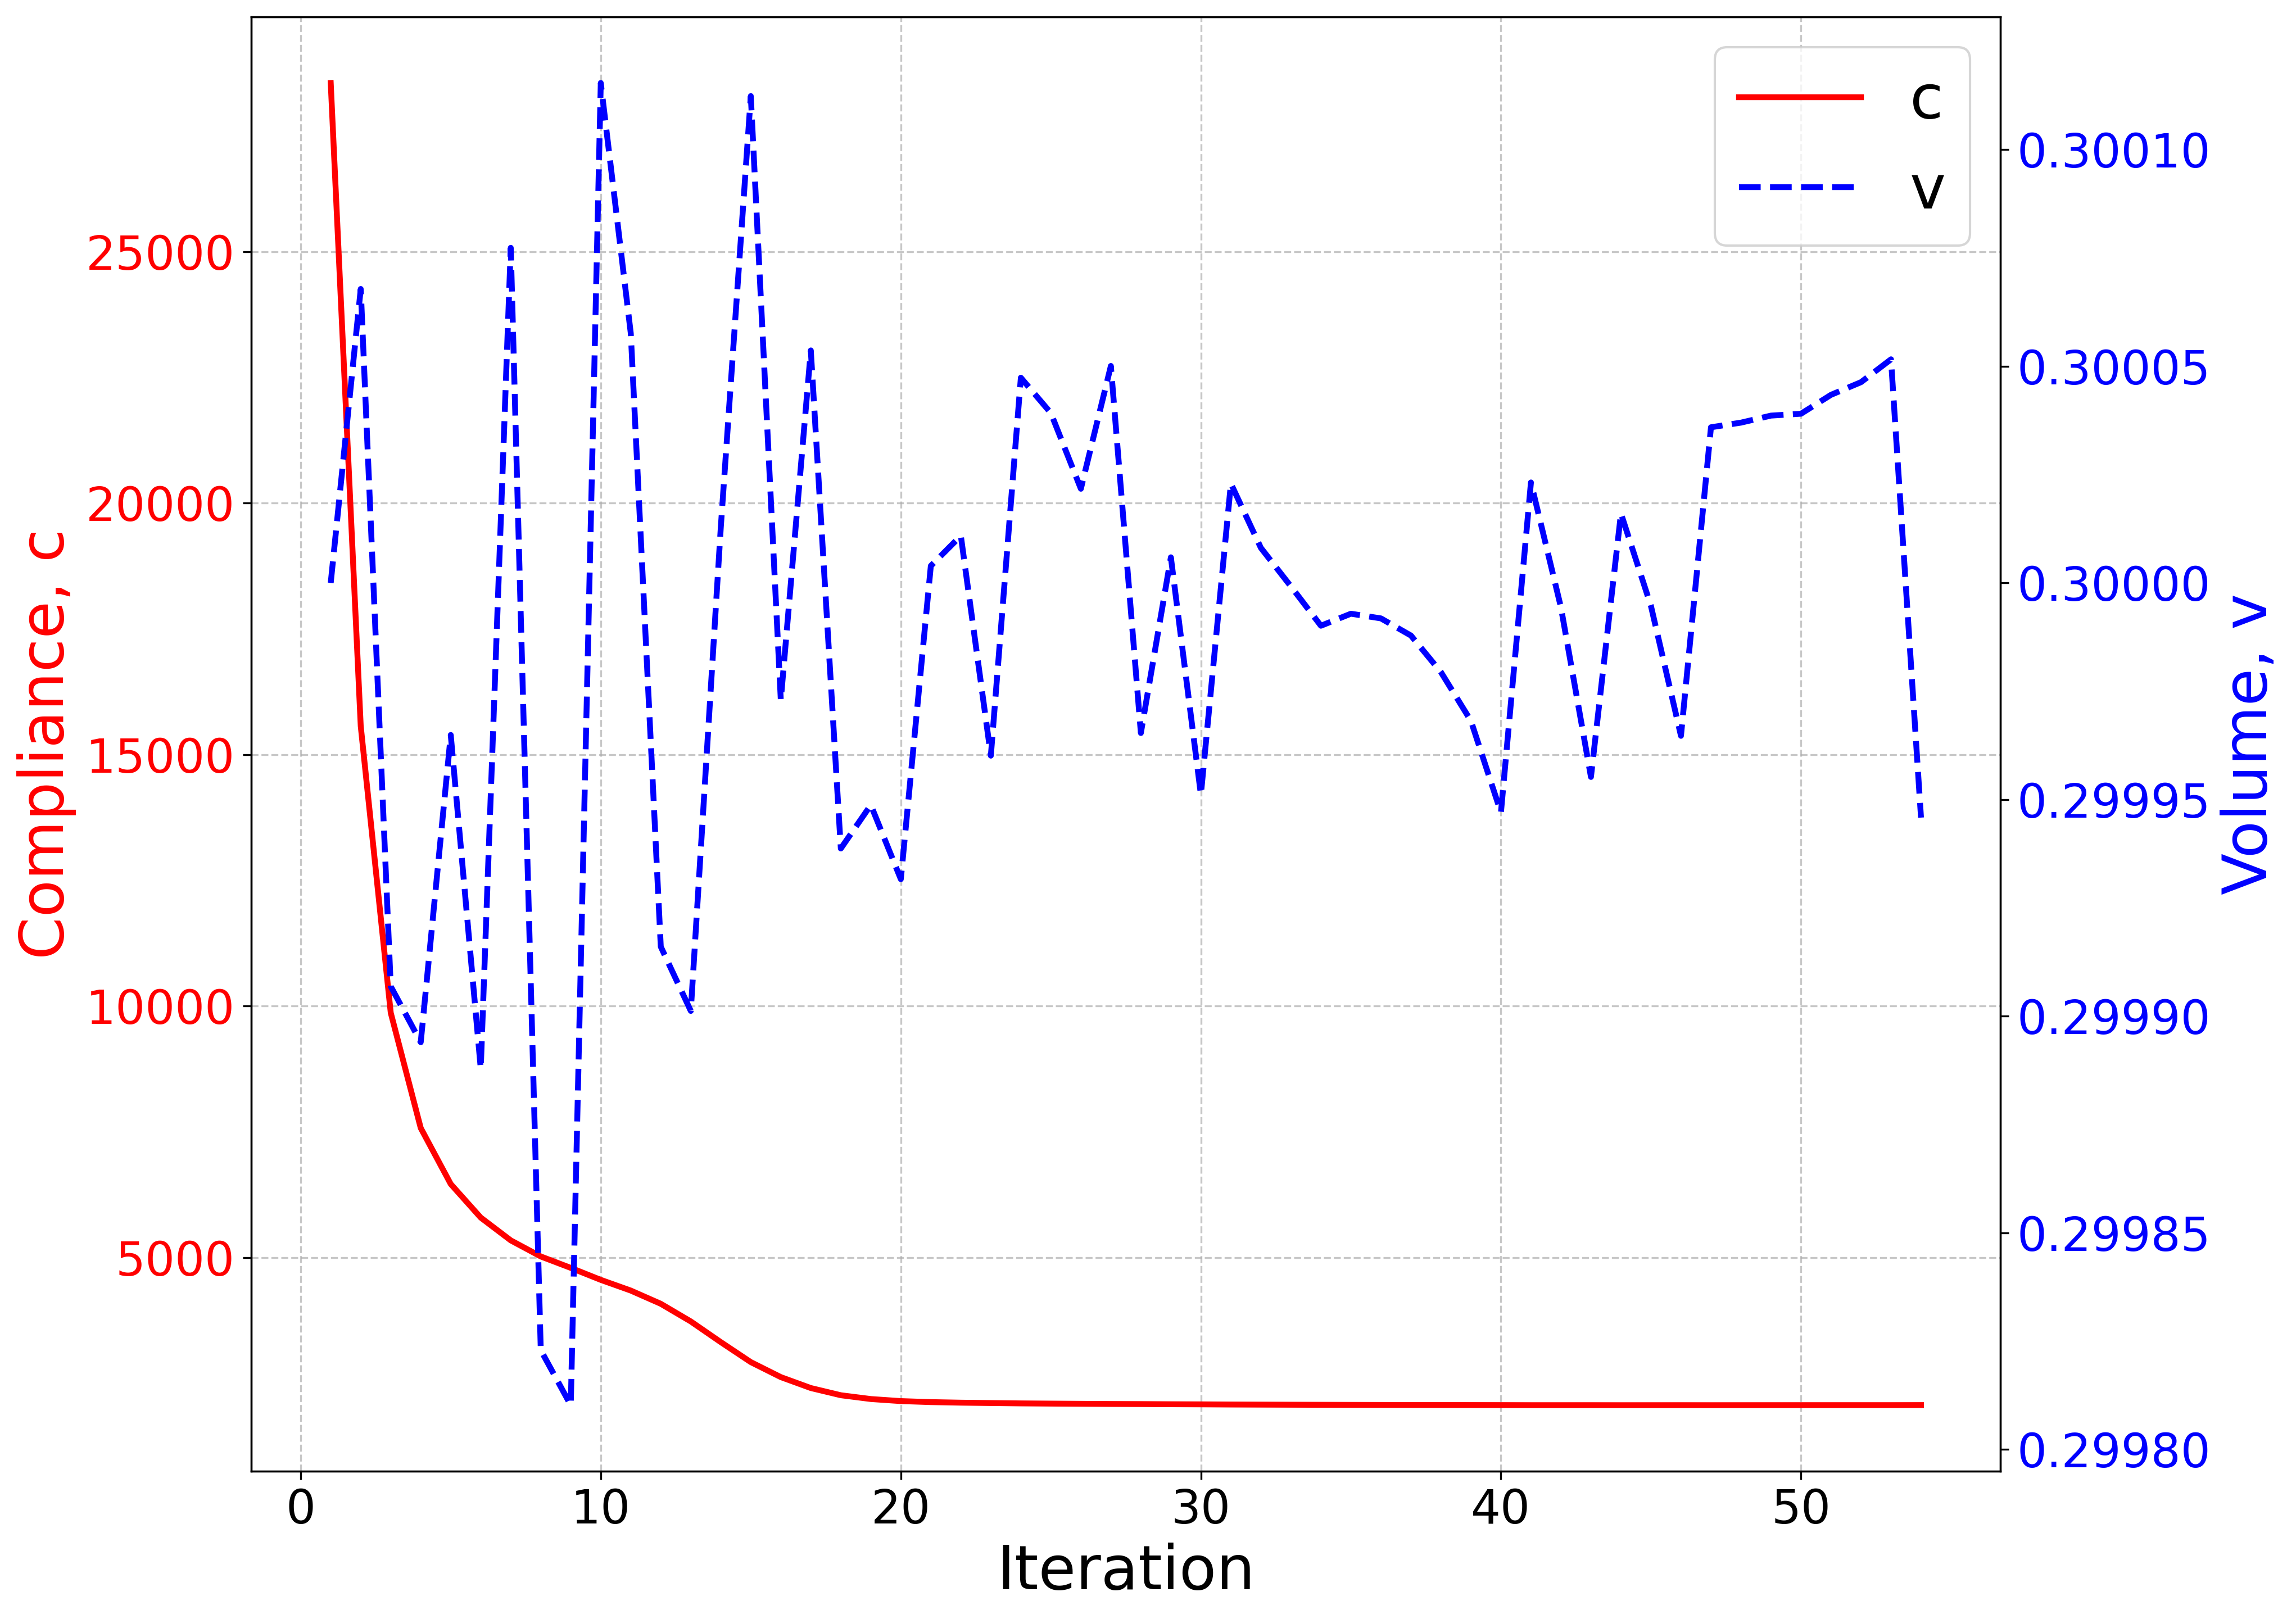
\includegraphics[width=0.85\textwidth]{figures/cantilever_3d_convergence_auto.png} \caption{Convergence histories of the compliance $c(\rho)$ and volume fraction $v(\rho)$ for the 3D cantilever beam optimization using automatic differentiation.} \label{fig:canti3d_ad_convergence} 
\end{figure}
\vspace{-2ex} % 可调节

To further illustrate the evolution of the topology during optimization, the layouts at selected iterations are shown in Figure~\ref{fig:canti3d_ad_topos}.
\vspace{-2ex} % 可调节
\begin{figure}[htp]
	\centering
	\subfloat[$c(\rho)=5338.9462,~v(\rho)=0.3001$]{
		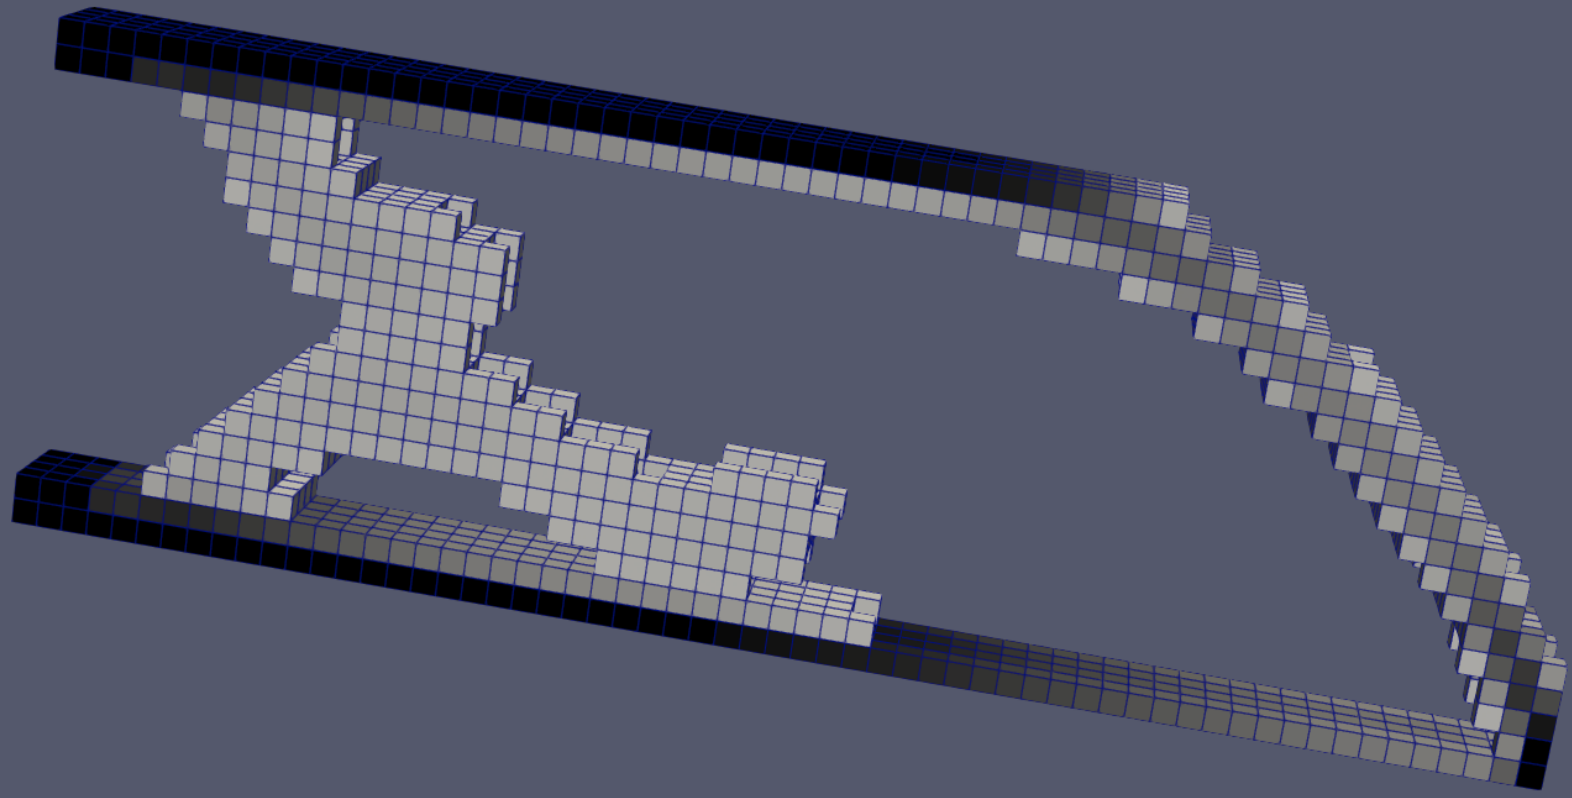
\includegraphics[width=0.32\textwidth]{figures/cantilever_3d_1_auto.png}
		\label{fig:canti3d_1_auto}
	}
	\subfloat[$c(\rho)=2122.6707,~v(\rho)=0.3000$]{
		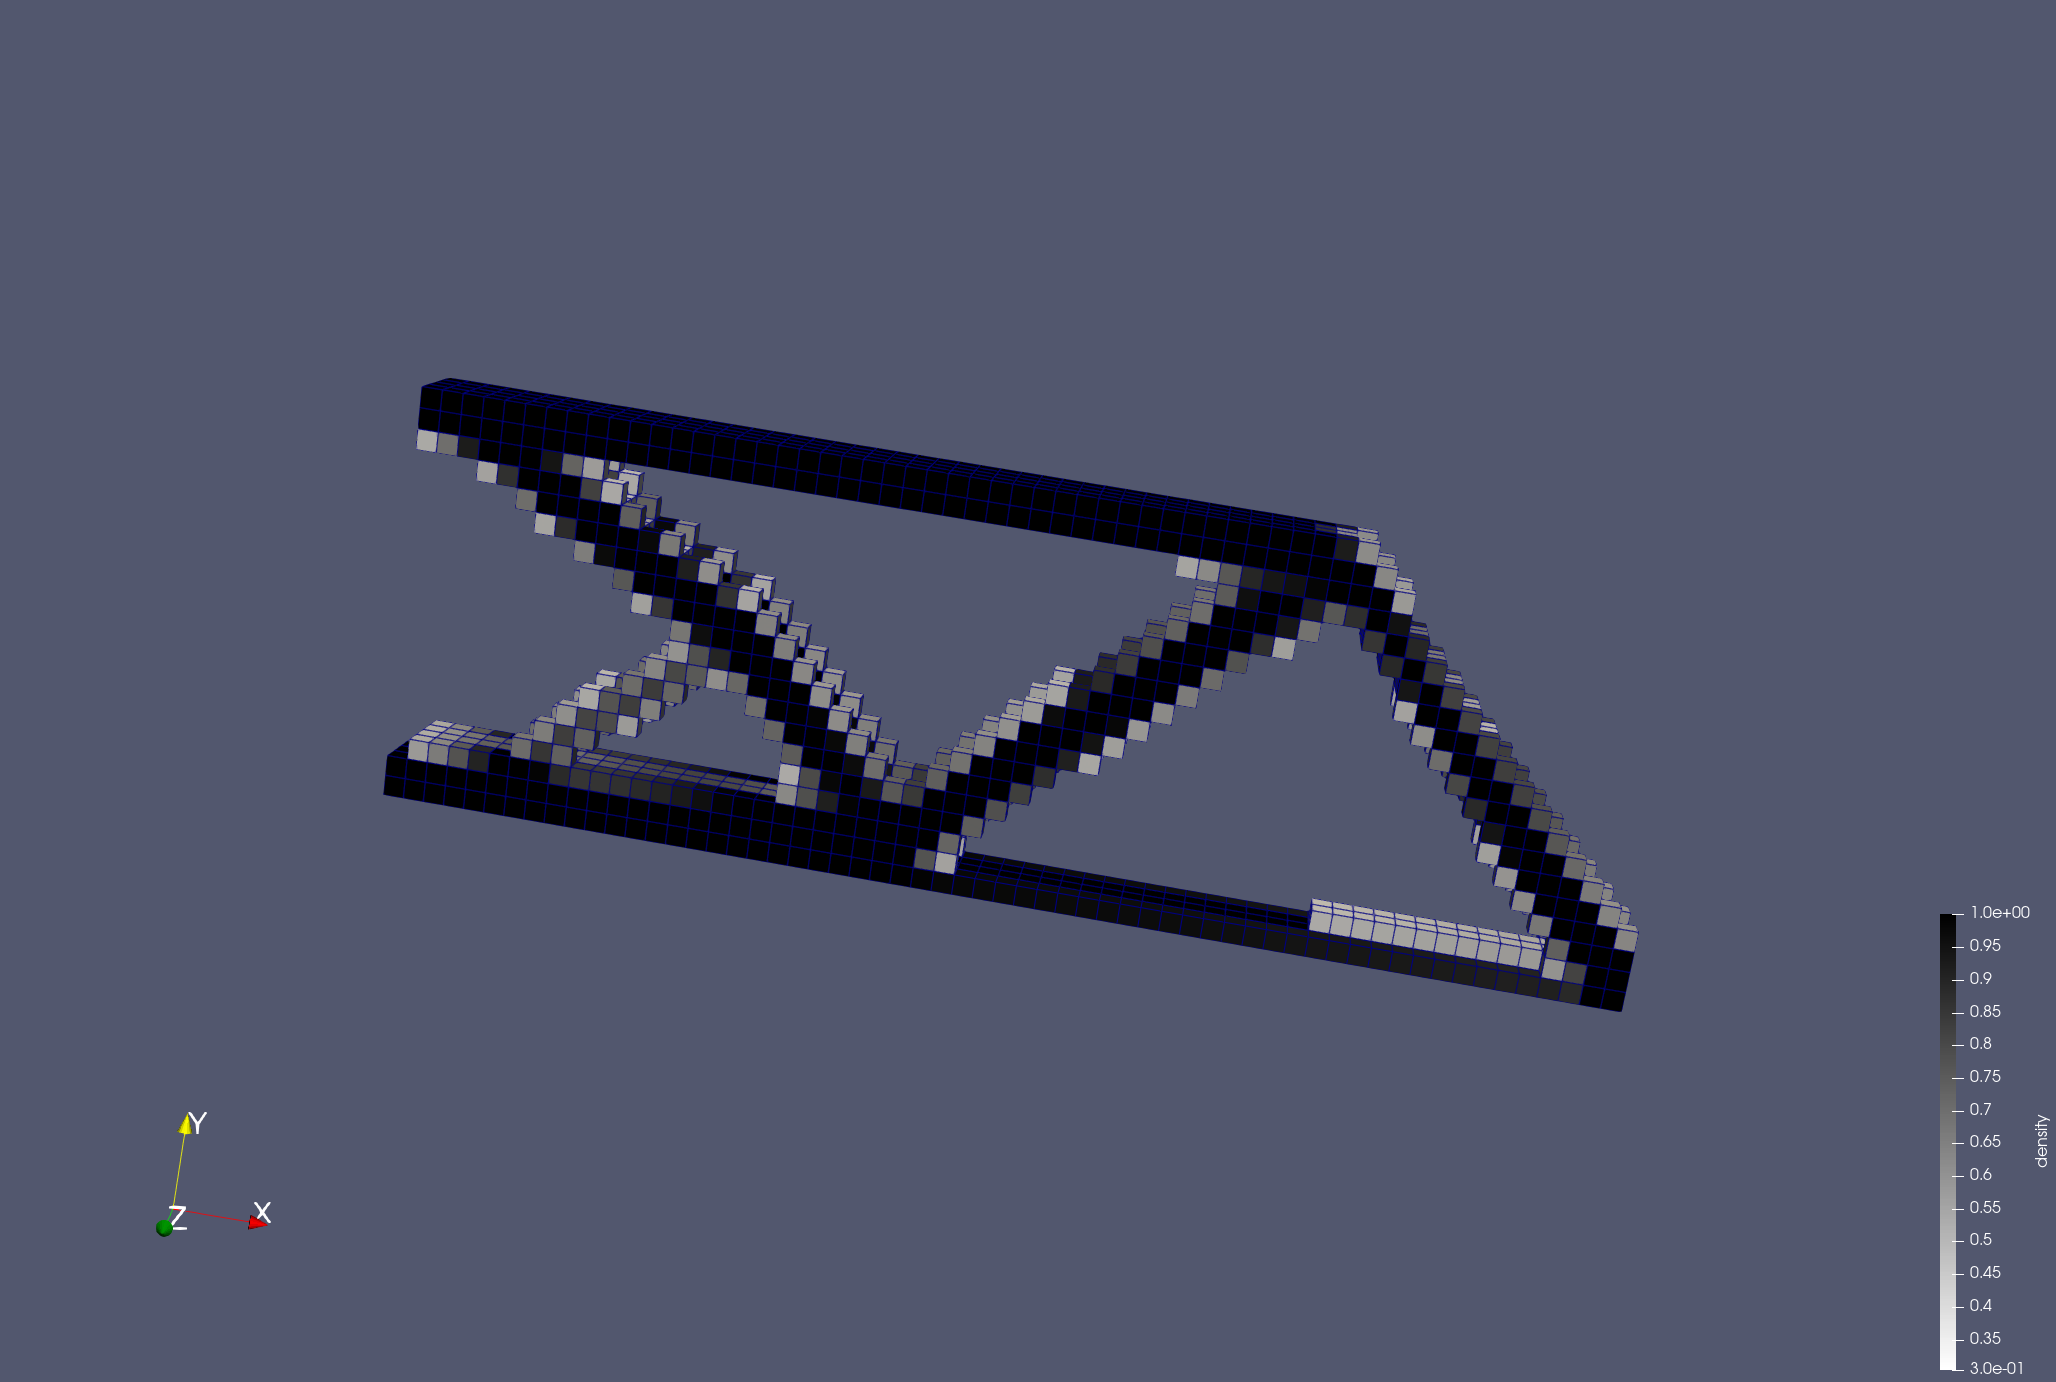
\includegraphics[width=0.32\textwidth]{figures/cantilever_3d_2_auto.png}
		\label{fig:canti3d_2_auto}
	}
	\subfloat[$c(\rho)=2063.5625,~v(\rho)=0.2999$]{
		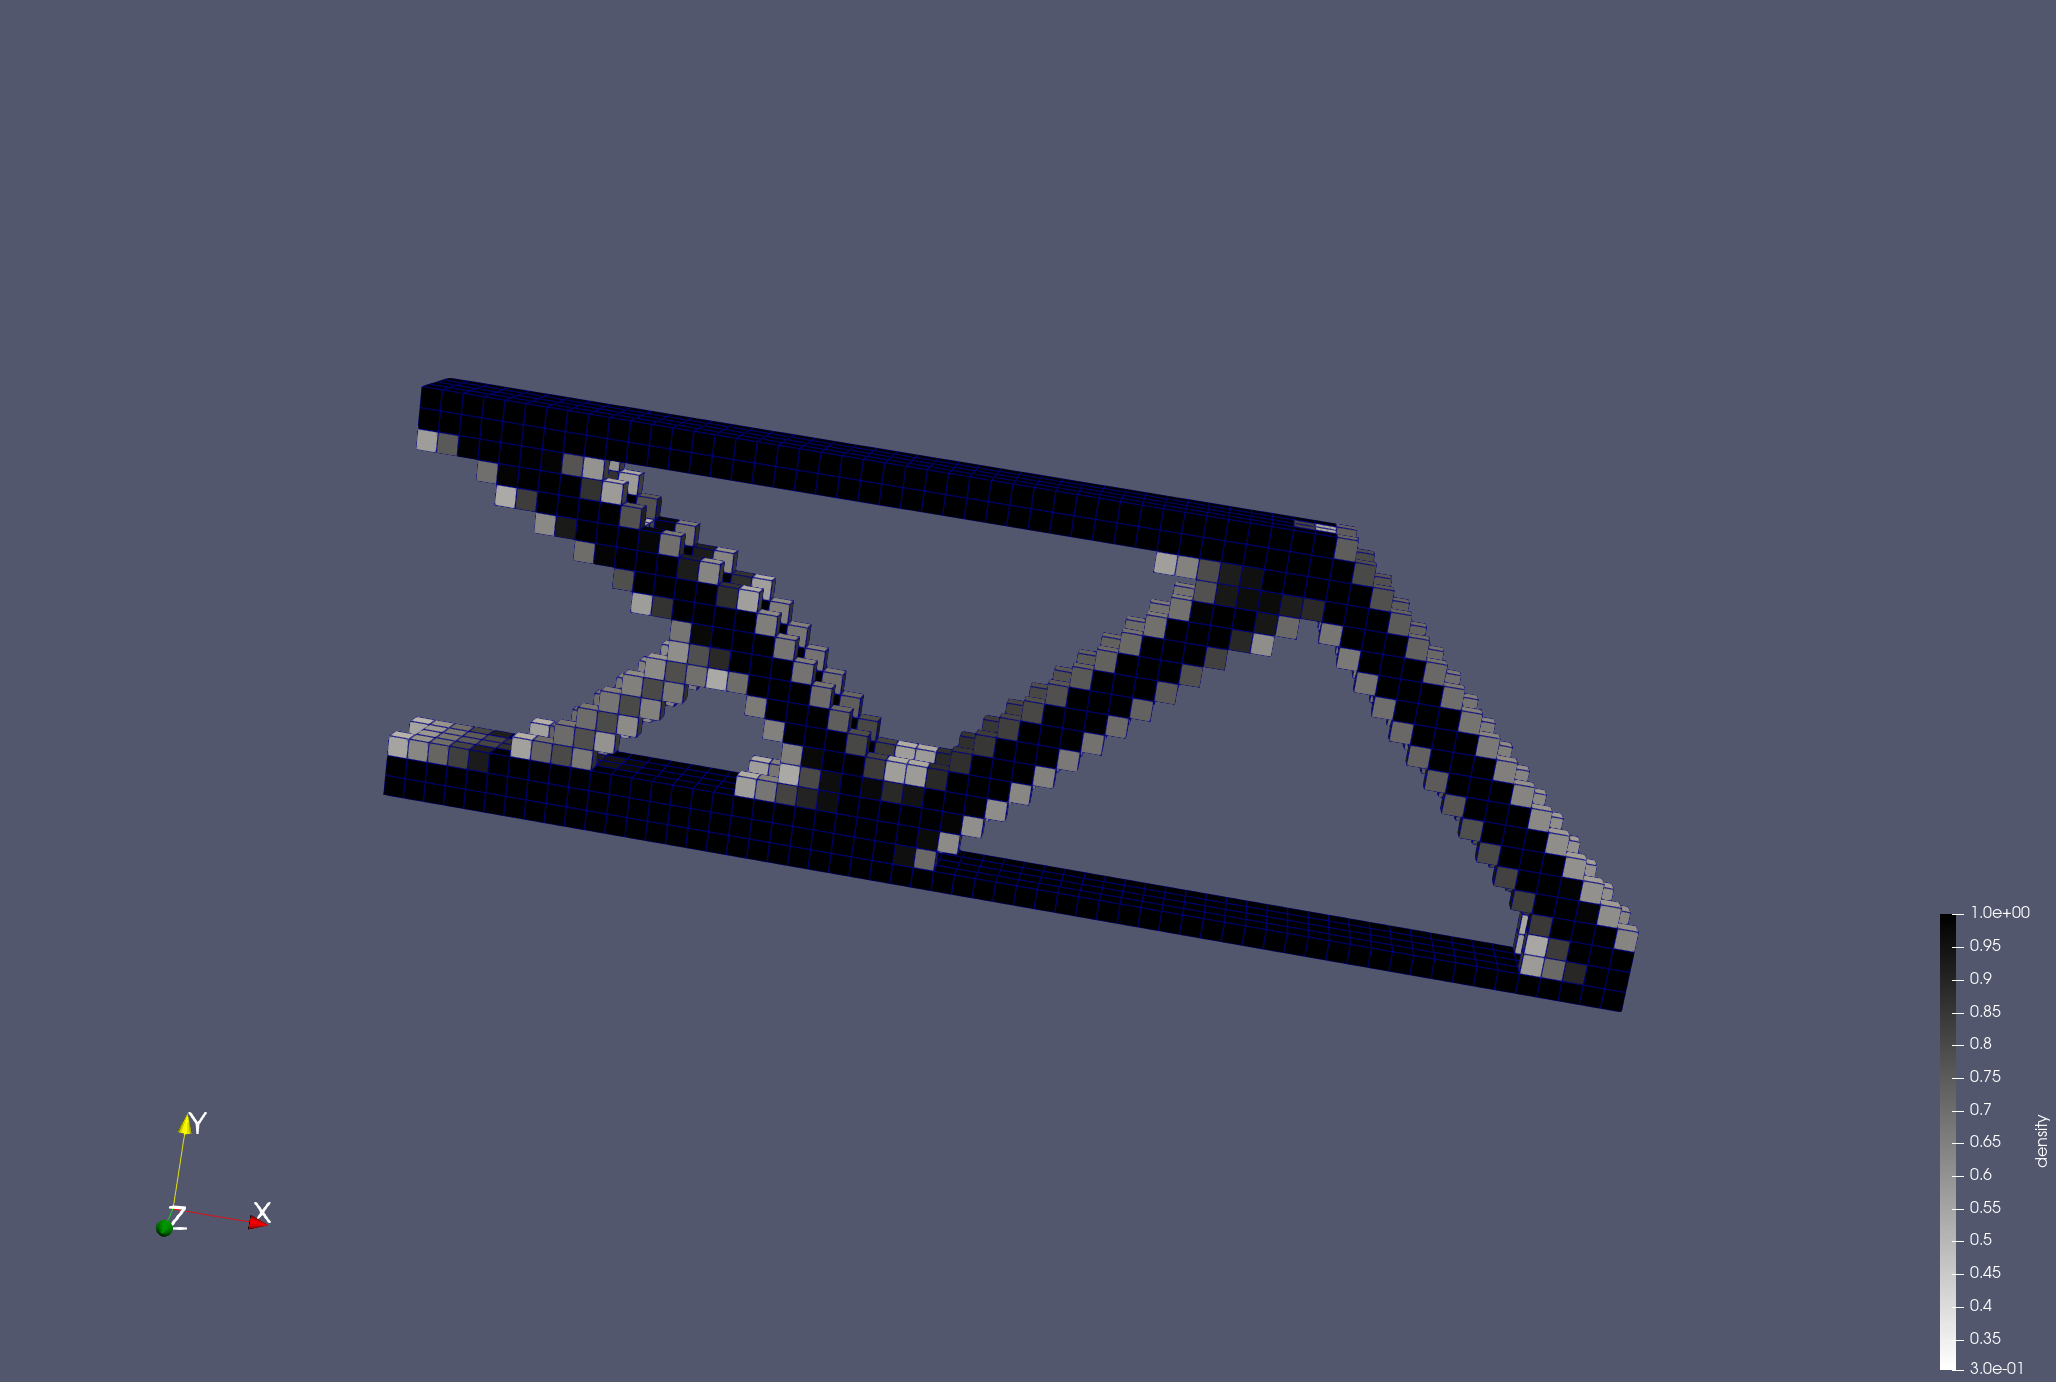
\includegraphics[width=0.32\textwidth]{figures/cantilever_3d_3_auto.png}
		\label{fig:canti3d_3_auto}
	}
	\caption{Topology layouts at iterations 7, 21, and 54 during the 3D cantilever beam optimization using AD. Only elements with $\rho>0.3$ are visualized. Each subfigure also reports the compliance and volume fraction.}
	\label{fig:canti3d_ad_topos}
\end{figure}
\vspace{-2ex} % 可调节

As observed from Figure~\ref{fig:canti3d_ad_convergence} and Figure~\ref{fig:canti3d_ad_topos}, the optimization results obtained using AD are fully consistent with those achieved through manual differentiation in Section~\ref{sec:exp_canti3d}. The compliance converges to approximately 2063.5625 after 54 iterations, and the volume fraction remains stably around 0.3. These results confirm that AD accurately computes the sensitivities and effectively guides the optimization process.

To evaluate the computational efficiency of AD, we compare the optimization times of AD and manual differentiation under the same 3D cantilever beam problem setting. As shown in Table~\ref{tab:ad_vs_manual}, the total optimization time and average iteration time for both methods are nearly identical, demonstrating that SOPTX’s AD implementation is highly efficient, introducing no significant computational overhead while maintaining the same high precision as manual differentiation.
\vspace{-0.5ex} % 可调节
\begin{table}[htbp]
	\centering
	\setlength{\tabcolsep}{4pt} % 减小列间距
	\caption{Performance comparison of differentiation methods in the 3D cantilever beam optimization problem.}
	%	\small % 使用小字体
	\begin{tabular}{ccccc}
		\toprule
		\textbf{Differentiation Method} & \textbf{Iterations} & \textbf{Total Time (s)} & \textbf{1st Iter. Time (s)} & \textbf{Avg. Iter. Time (s)} \\
		\midrule
		Manual Differentiation & 54 & 39.562 & 1.940 & 0.710 \\
		AD & 54 & 39.865 & 1.832 & 0.718 \\
		\bottomrule
	\end{tabular}
	\label{tab:ad_vs_manual}
\end{table}
\vspace{-0.5ex} % 可调节

In addition to PyTorch, SOPTX also supports the JAX backend~\cite{bradbury2018jax}, which offers equally powerful AD capabilities. The sensitivity computation code remains identical when using JAX, users simply need to switch to the JAX backend by executing:
\vspace{-0.5ex} % 可调节
\begin{lstlisting}[language=python]
bm.set_backend('jax')
\end{lstlisting}
\vspace{-0.5ex} % 可调节

Using AD with the JAX backend, we perform topology optimization for the 3D cantilever beam, achieving results fully consistent with those from the PyTorch backend. This consistency underscores the stability and flexibility of the SOPTX framework across different computational backends. The final optimized topology is shown in Figure~\ref{fig:canti3d_ad_jax}.
\vspace{-2ex} % 可调节
\begin{figure}[htp] 
	\centering 
	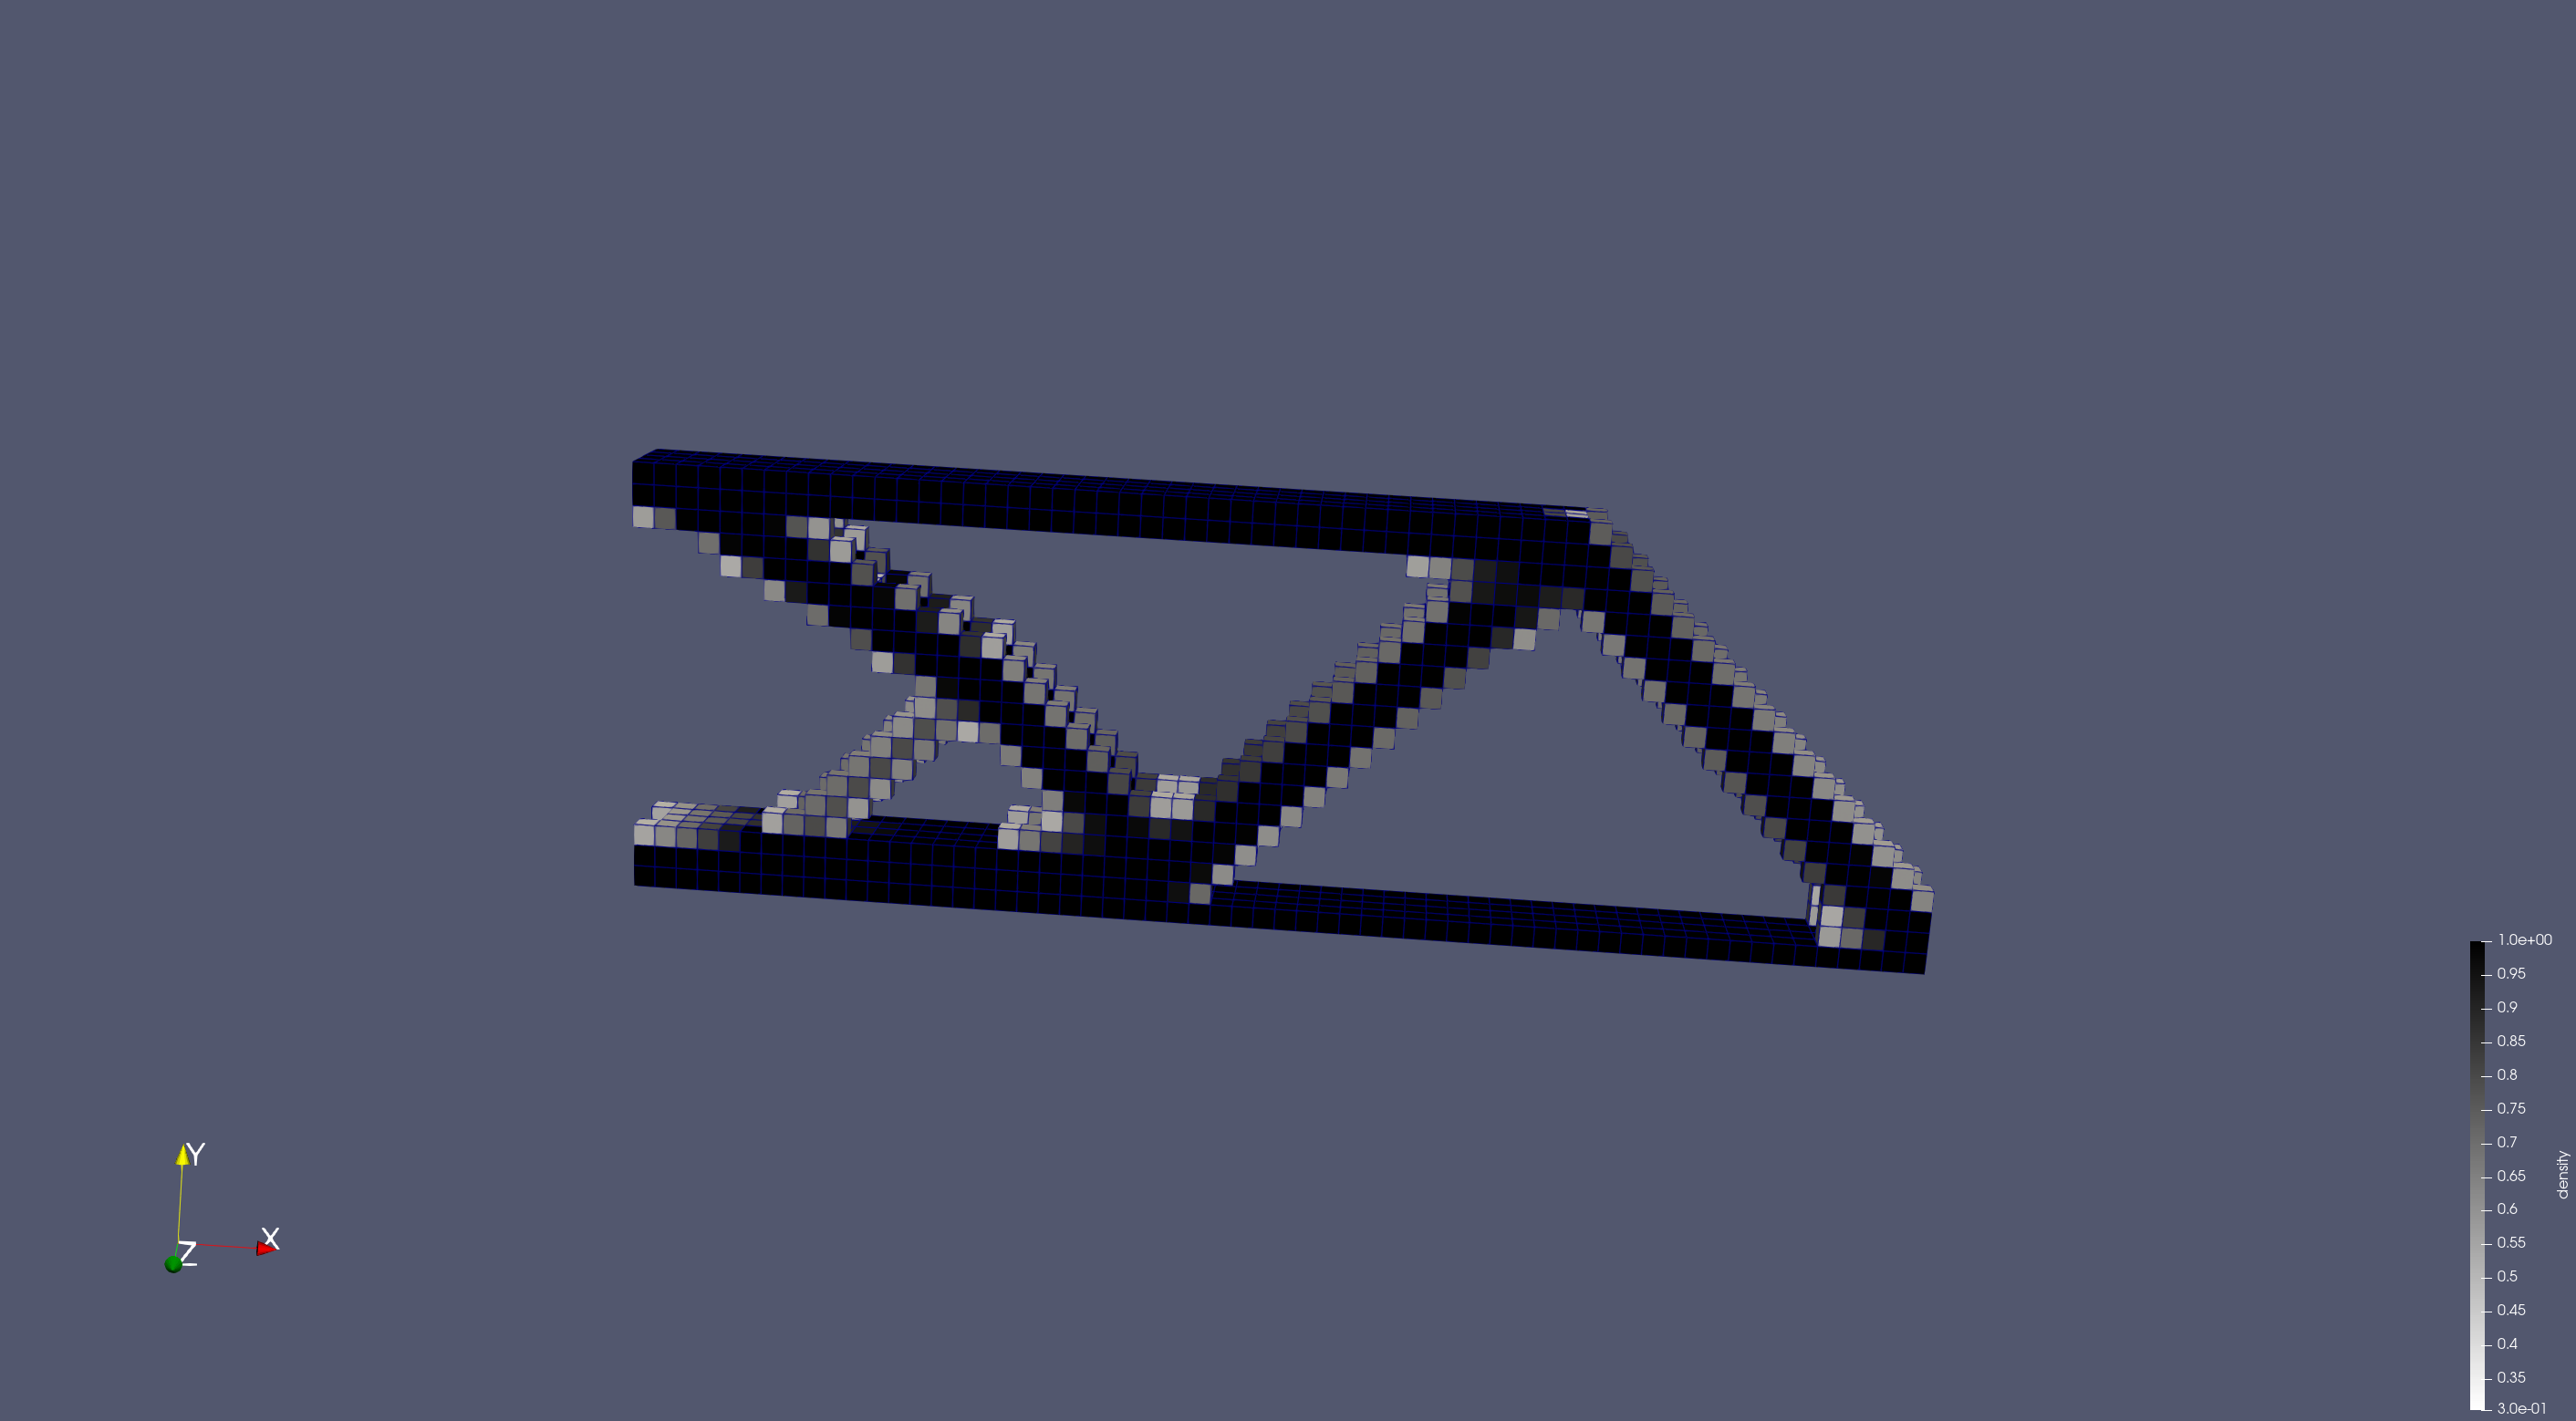
\includegraphics[width=0.75\textwidth]{figures/cantilever_3d_auto_jax.png} \caption{Final optimized topology of the 3D cantilever beam using AD with the JAX backend.} \label{fig:canti3d_ad_jax} 
\end{figure}
\vspace{-2ex} % 可调节

The application of AD in TO offers several significant advantages:
\vspace{-0.5ex} % 可调节
\begin{itemize} 
	\item \textbf{Simplified Model Switching}: In TO, the choice of material interpolation model directly influences the optimization results. Besides the commonly used SIMP model, alternative models such as RAMP~\cite{stolpe2001alternative} are also widely applied in specific scenarios. With AD, users can easily switch between different interpolation models. For instance, when switching from SIMP to RAMP, the material stiffness gradient can be automatically computed by AD without manually deriving complex formulas. This greatly improves development efficiency and enhances the flexibility of model experimentation.
	\item \textbf{Seamless Constraint Switching}: TO often involves multiple constraints. In addition to volume constraints, manufacturing constraints such as length scale control~\cite{guest2009imposing}, connectivity~\cite{li2016structural}, overhang limitations~\cite{qian2017undercut}, and material usage restrictions~\cite{sanders2018multi} are frequently imposed. Traditionally, adding or modifying constraints requires manually re-deriving sensitivity expressions. By introducing AD, this process becomes fully automated. The system can seamlessly adapt to new constraint settings, significantly improving optimization adaptability and development efficiency.
	\item \textbf{Support for Complex Problems}: For TO problems involving multiphysics coupling, nonlinear materials, or complex geometric constraints, AD efficiently handles the computation of complicated gradients, allowing users to focus on modeling rather than mathematical derivations. Moreover, AD can automatically manage combined sensitivity computations when using techniques like density filtering and Heaviside projection. This capability further enhances the practical applicability and flexibility of the SOPTX framework in complex engineering scenarios.
\end{itemize}
\vspace{-0.5ex} % 可调节

Through the optimization example of the 3D cantilever beam, this section has demonstrated the powerful potential of AD within the SOPTX framework. Numerical results show that AD achieves comparable precision and computational efficiency to traditional manual differentiation methods without introducing any significant overhead. The multi-backend support of SOPTX, including PyTorch and JAX, further enhances the flexibility and scalability of the framework. The application of AD not only simplifies sensitivity analysis but also facilitates the exploration of novel material models and constraint conditions. These features make SOPTX a valuable tool in the field of topology optimization, providing robust support for education, research, and engineering applications.

\subsection{Multi-Backend Switching}\label{sec:exp_multi_backend}
The SOPTX framework supports multi-backend switching, currently offering three computational backends: NumPy, PyTorch, and JAX. Backend switching is managed through the \textit{Tensor Backend Manager}, and users can easily switch between different backends by using the \texttt{set\_backend} function:
\vspace{-0.5ex} % 可调节
\begin{lstlisting}[language=python]
bm.set_backend('numpy')    
bm.set_backend('pytorch') 
bm.set_backend('jax')     
\end{lstlisting}
\vspace{-0.5ex} % 可调节

To verify the consistency and reliability of SOPTX across different computational backends, we conduct tests on the 3D cantilever beam optimization problem described in Sections~\ref{sec:exp_canti3d} and~\ref{sec:exp_canti3d_ad}, using identical parameter settings. The problem is solved separately under the NumPy, PyTorch, and JAX backends. The optimization results show that the convergence histories and final topology layouts are highly consistent across all three backends:
\vspace{-2ex} % 可调节
\begin{figure}[htp]
	\centering
	\subfloat[$c(\rho)=2063.5625,~v(\rho)=0.2999$]{
		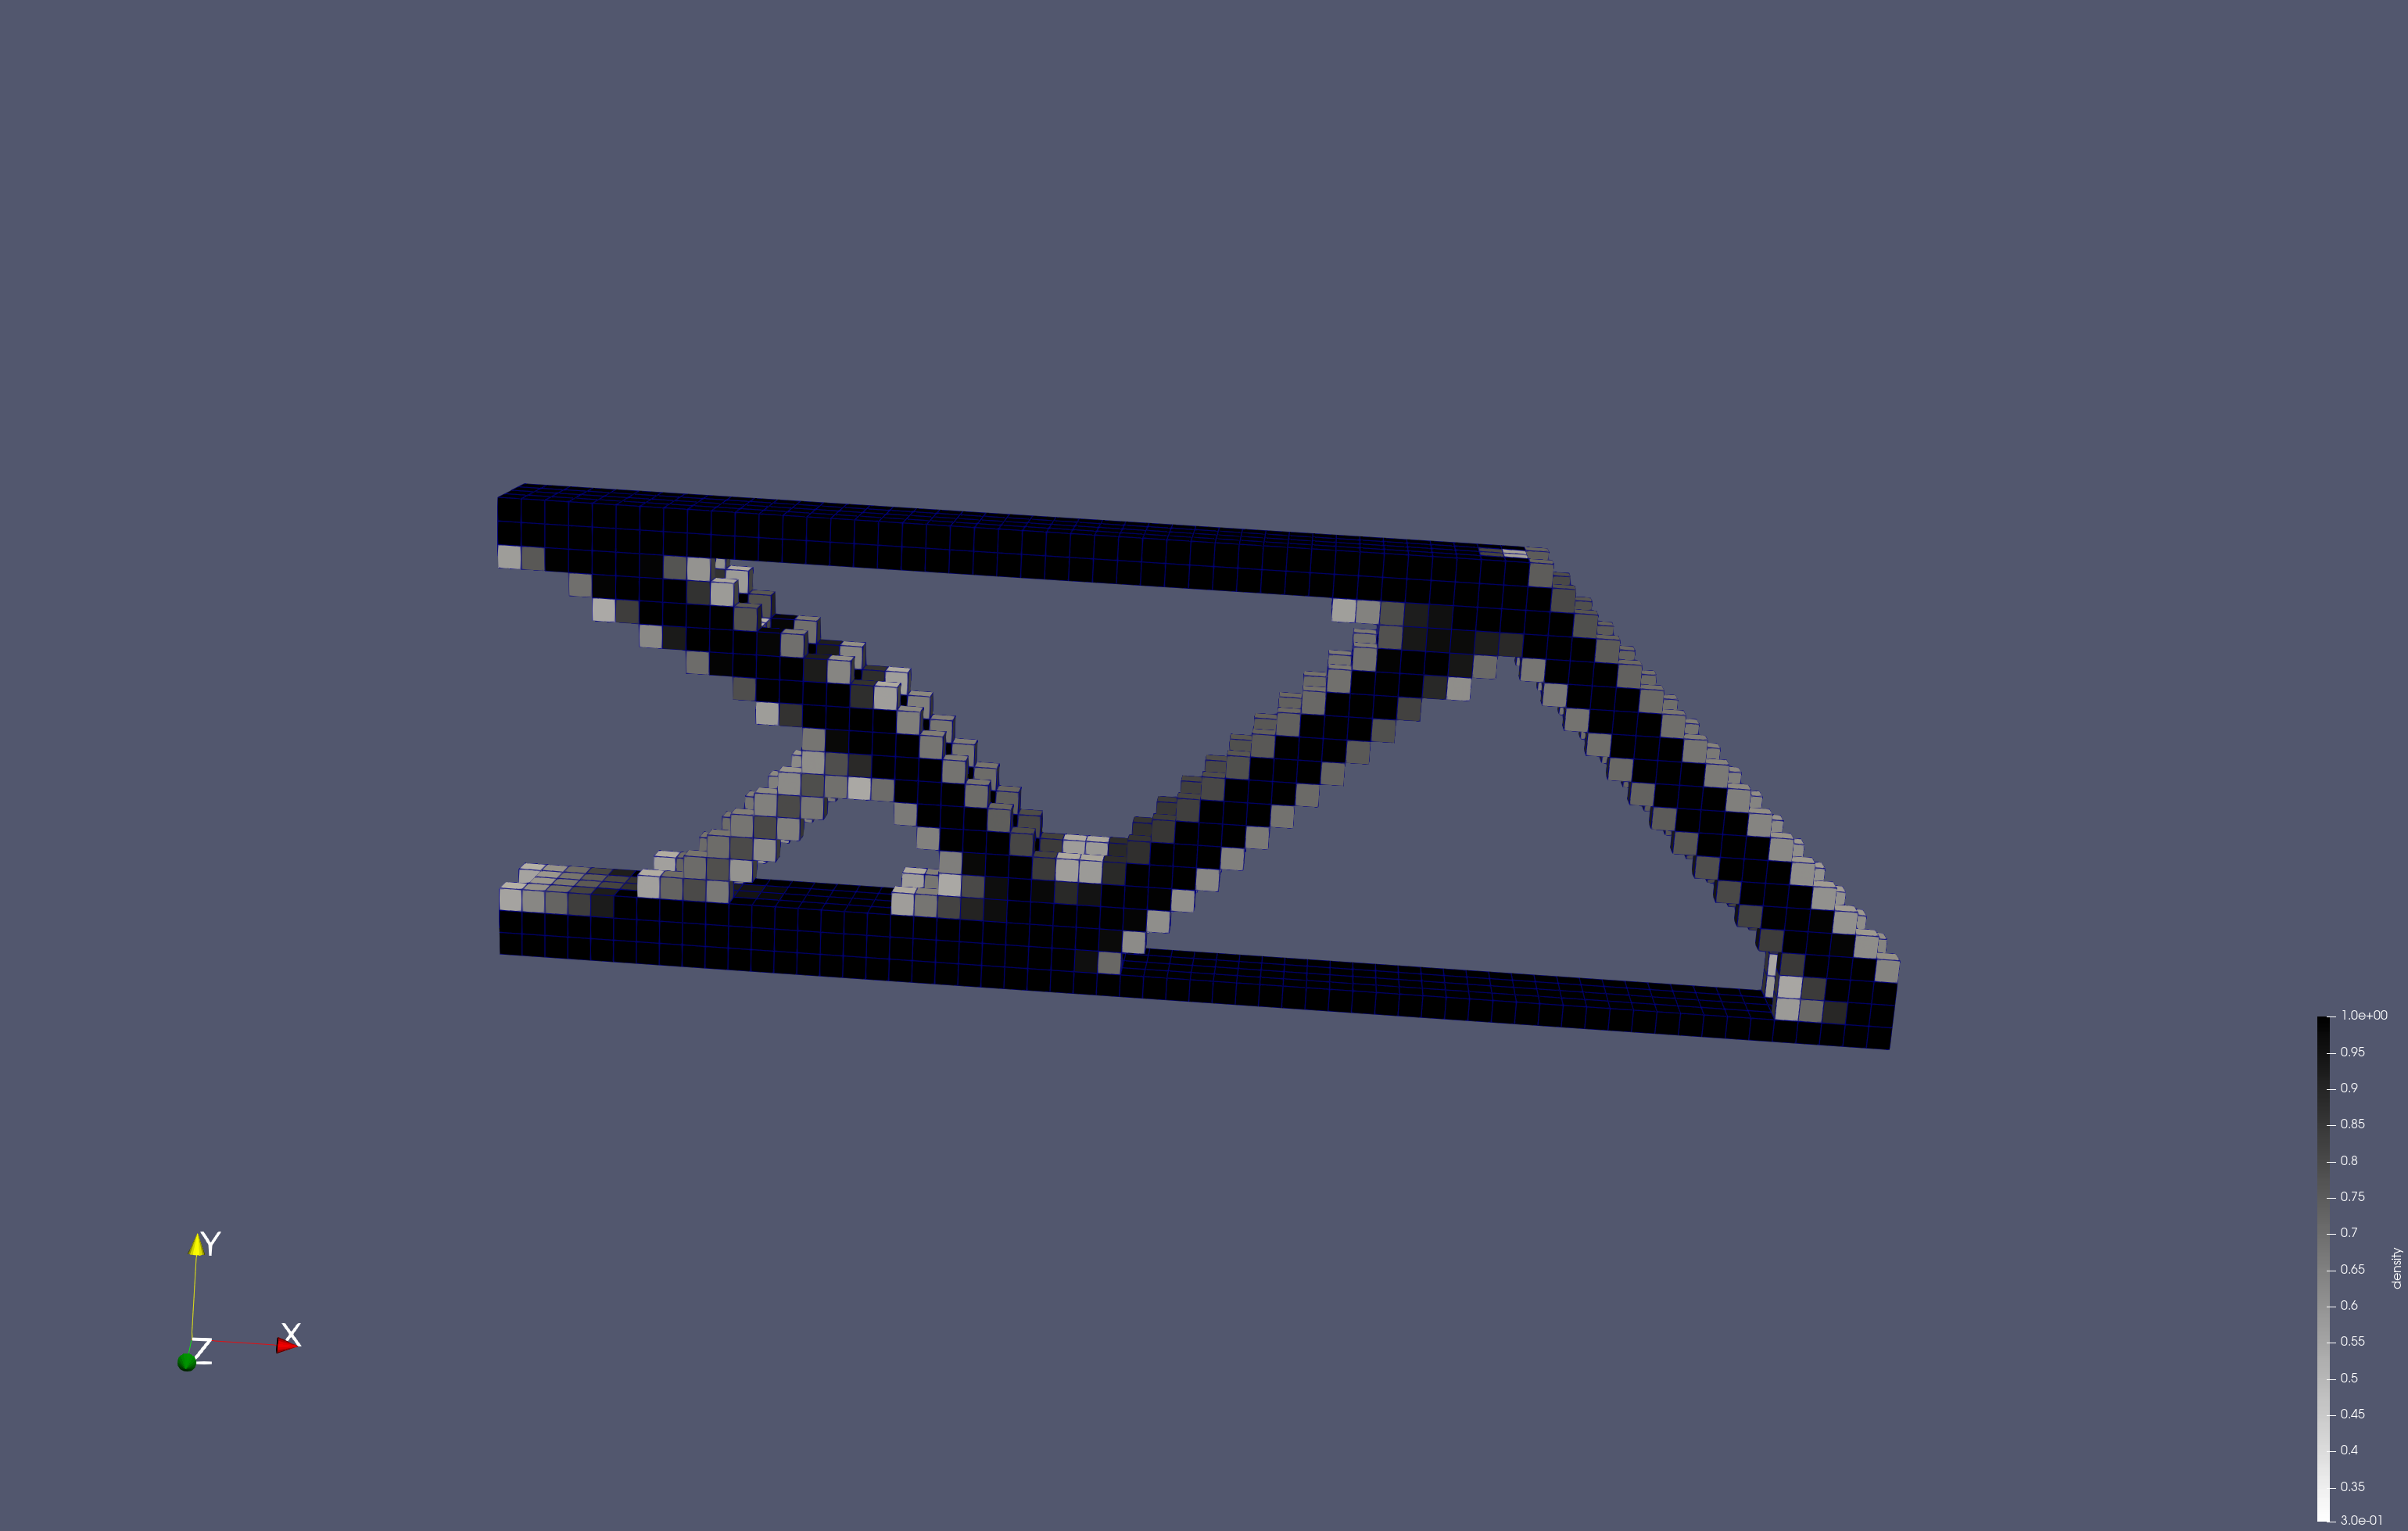
\includegraphics[width=0.32\textwidth]{figures/cantilever_3d_np.png}
		\label{fig:canti3d_np}
	}
	\subfloat[$c(\rho)=2063.5625,~v(\rho)=0.2999$]{
		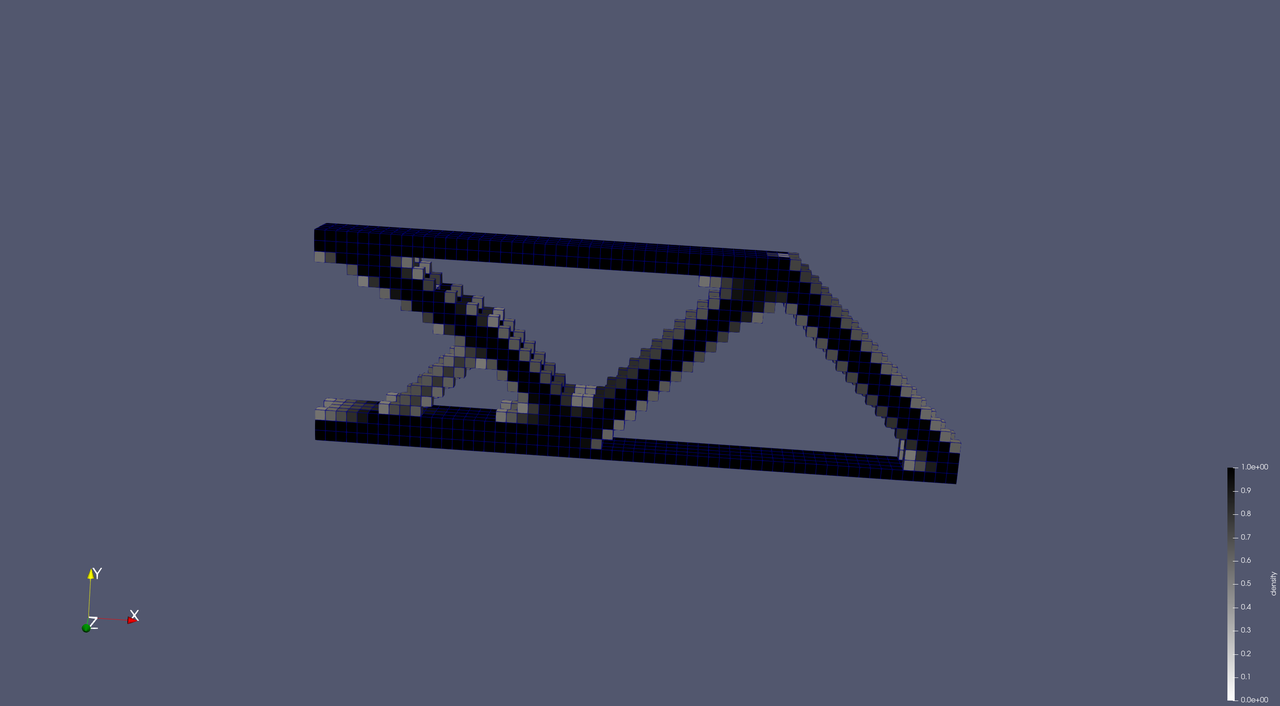
\includegraphics[width=0.32\textwidth]{figures/cantilever_3d_torch.png}
		\label{fig:canti3d_torch}
	}
	\subfloat[$c(\rho)=2063.5625,~v(\rho)=0.2999$]{
		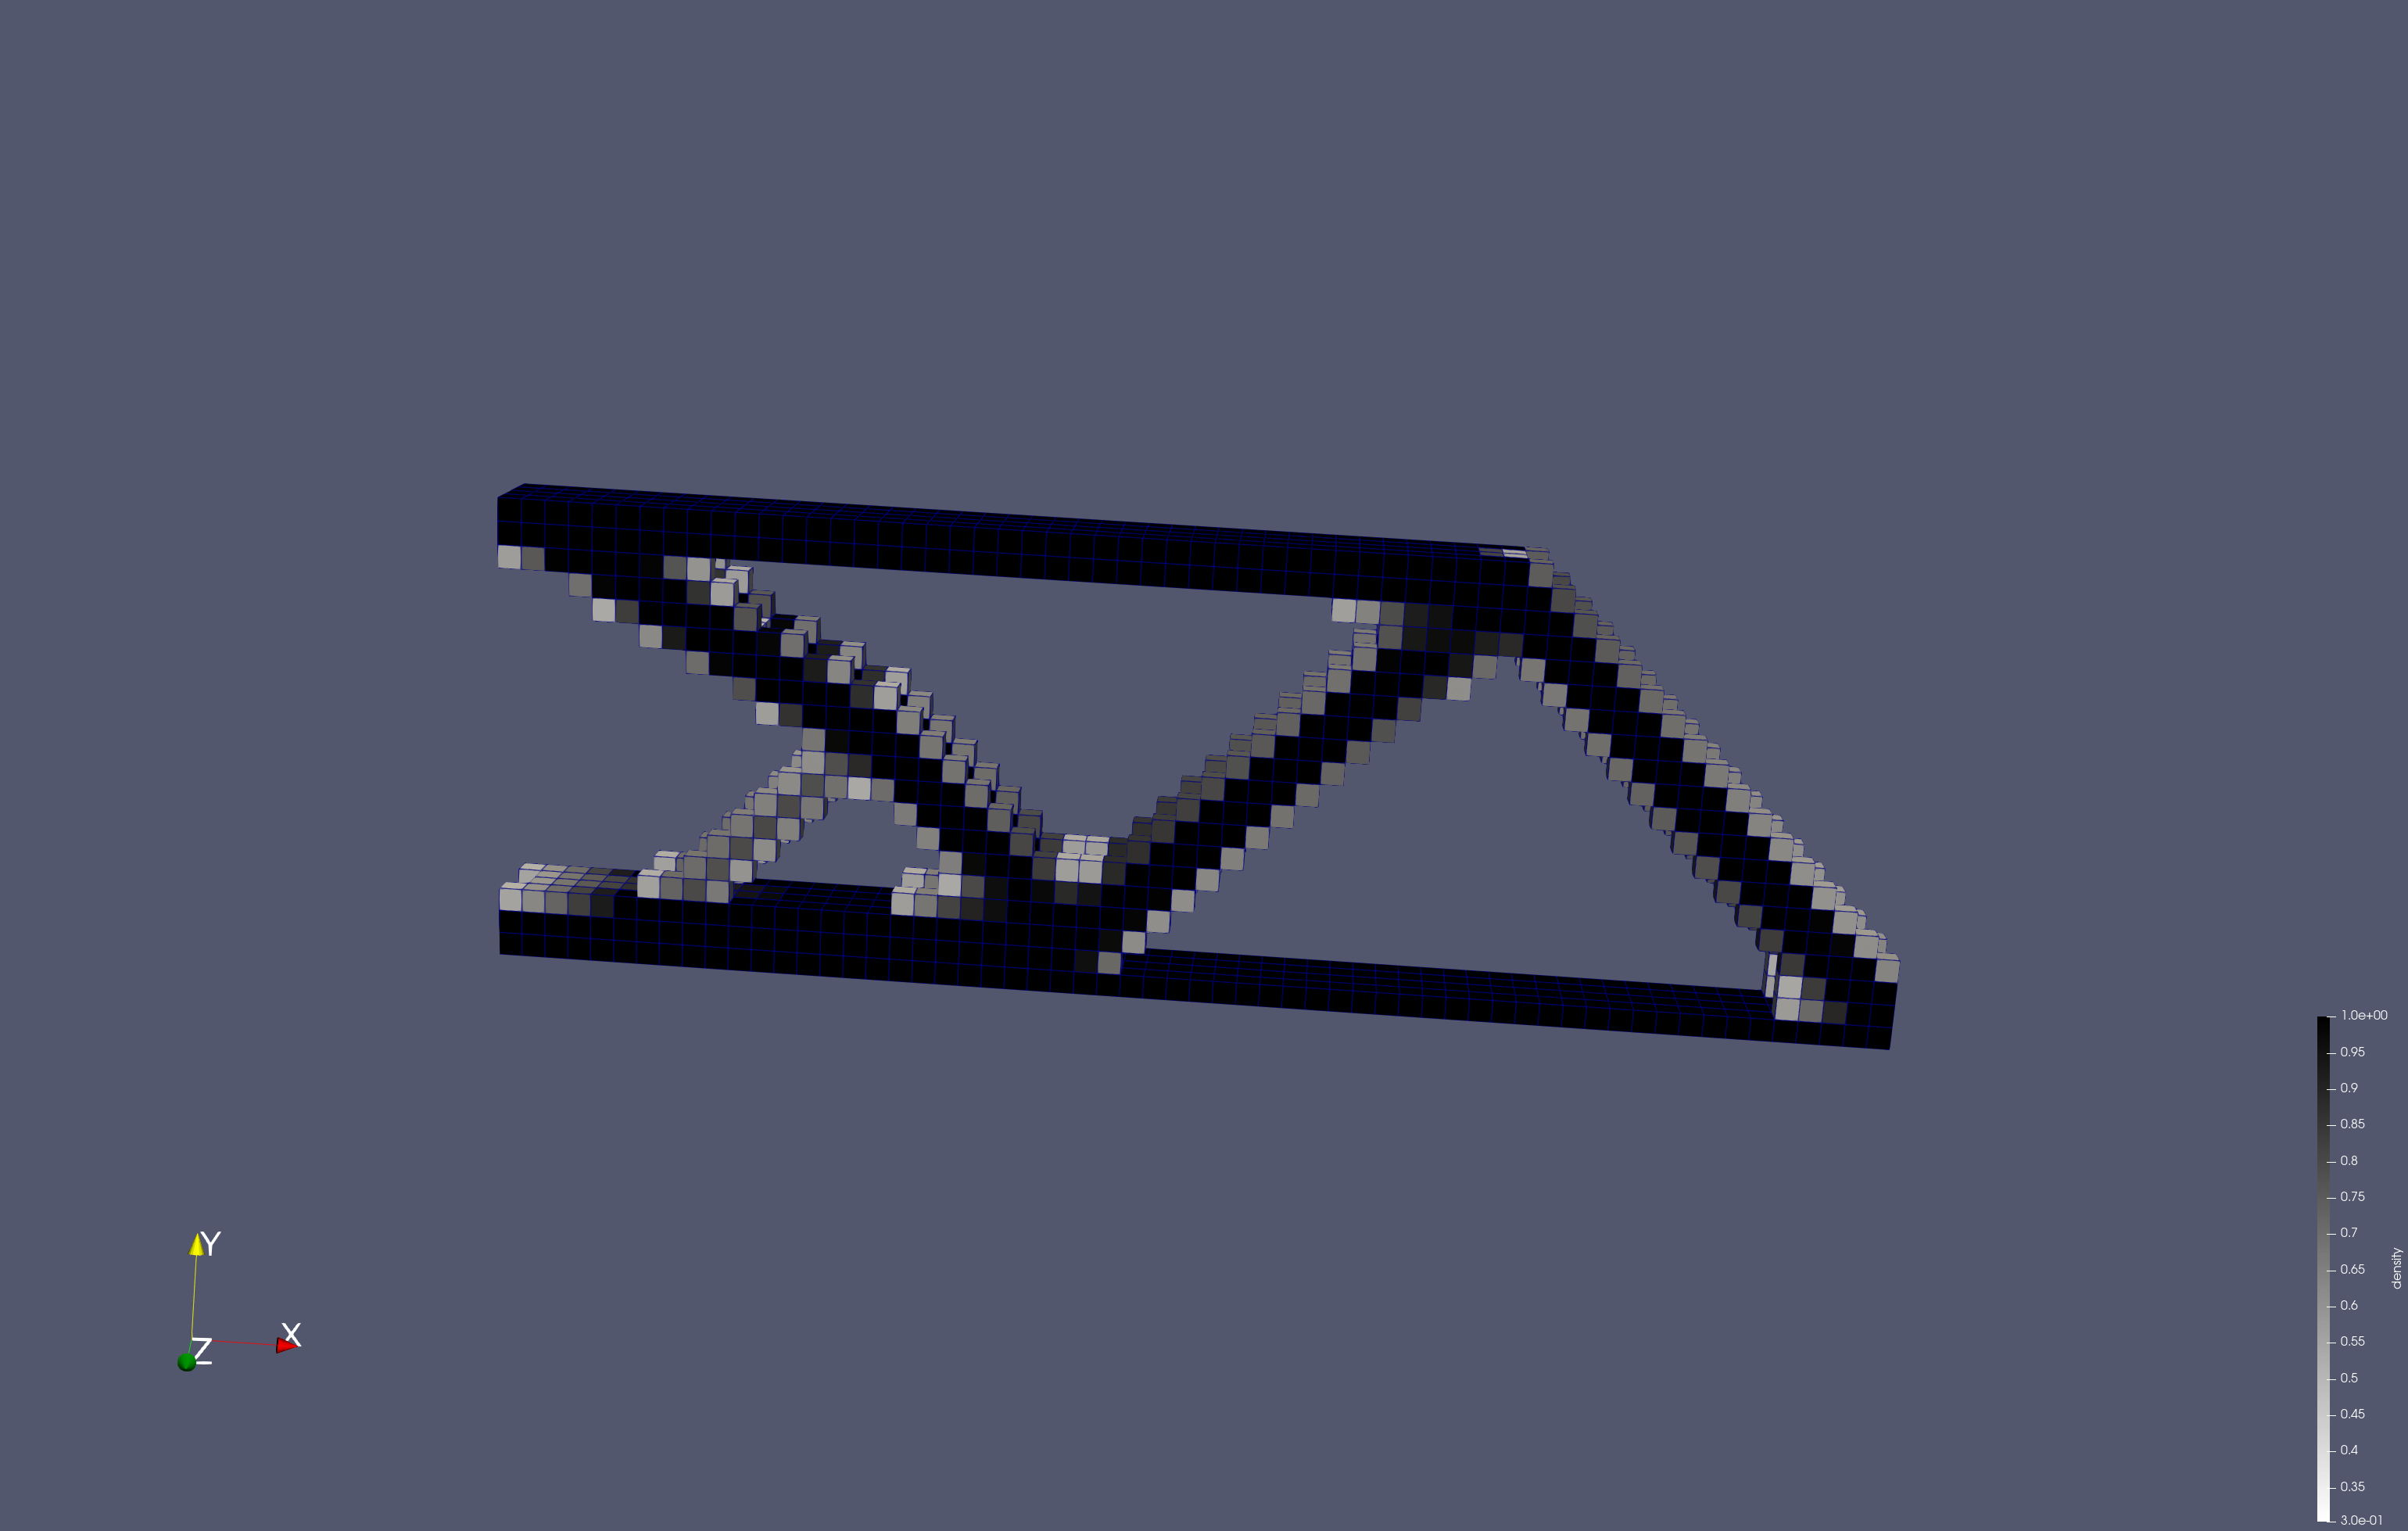
\includegraphics[width=0.32\textwidth]{figures/cantilever_3d_jax.png}
		\label{fig:canti3d_jax}
	}
	\caption{Final optimized topologies of the 3D cantilever beam using three different backends (elements with $\rho>0.3$ are visualized). Left: NumPy backend; Middle: PyTorch backend; Right: JAX backend.}
	\label{fig:canti3d_backend_compare}
\end{figure}
\vspace{-2ex} % 可调节

As shown in Figure~\ref{fig:canti3d_backend_compare}, after 54 iterations, the compliance in all three backends converges to approximately $2063.5625$, and the volume fraction stabilizes around 0.3. The final topology layouts are nearly identical. This consistency highlights the effectiveness of SOPTX's unified numerical abstraction and rigorous testing strategy, ensuring the reliability and stability of the algorithms across different computational backends.

In addition to multi-backend switching, SOPTX also supports computations on GPUs to further enhance computational efficiency, especially when solving large-scale 3D TO problems. By default, all computations are performed on the CPU (\texttt{device='cpu'}). However, users can migrate computations to the GPU (e.g., CUDA devices) through two methods:
\vspace{-0.5ex} % 可调节
\begin{enumerate}
	\item \textbf{Set the Default Device Globally}: Users can set the default device for all tensors globally by executing:
\begin{lstlisting}[language=python]
bm.set_default_device('cuda')
\end{lstlisting}
	This method places all subsequently created tensors on the GPU by default, and all associated computations, such as matrix assembly and linear solving, are performed on the GPU.
	\item \textbf{Specify the Device When Creating the Mesh}: Alternatively, users can specify the device during mesh initialization:
\begin{lstlisting}[language=python]
mesh = UniformMesh3d(extent=extent, h=h, origin=origin, device='cuda')
\end{lstlisting}
	By specifying \texttt{device='cuda'} during mesh creation, all computations related to that mesh are performed on the GPU. This approach offers greater flexibility, allowing users to mix CPU and GPU computations within the same program if needed.
\end{enumerate}
\vspace{-0.5ex} % 可调节

GPU acceleration plays a crucial role in 3D TO, as computational complexity increases significantly with the growth of mesh size. Taking the 3D cantilever beam example from Section~\ref{sec:exp_canti3d} as a reference, when the mesh size is doubled to $120\times40\times8$, the number of density design variables rises to $38,400$, and the number of displacement degrees of freedom reaches $133,947$. On the CPU, the optimization process becomes much more time-consuming due to the computational cost associated with matrix assembly and linear solving. In contrast, the parallel computing capability of GPUs can substantially improve efficiency and significantly reduce computation time.

To intuitively demonstrate the effect of GPU acceleration, we compare the computation times between CPU and GPU under the PyTorch backend for the same 3D cantilever beam problem. The parameter settings are kept identical to those in Section~\ref{sec:exp_canti3d}, except that the filter radius is increased from 
$1.5$ to $3.0$ to ensure structural smoothness given the enlarged physical domain. Additionally, considering the increased problem size, we switch the linear solver from a direct method (e.g., MUMPS) to an iterative method, namely the Conjugate Gradient (CG) method. The CG method offers advantages for solving large-scale sparse linear systems and can leverage the GPU's parallel computing capabilities to efficiently perform matrix-vector operations.

The tests are conducted on an AMD 9950X CPU and an NVIDIA 5070Ti GPU. The optimization results are shown below:
\begin{figure}[htp]
	\centering
	\subfloat[$c(\rho)=3498.8266,~v(\rho)=0.3001$]{
		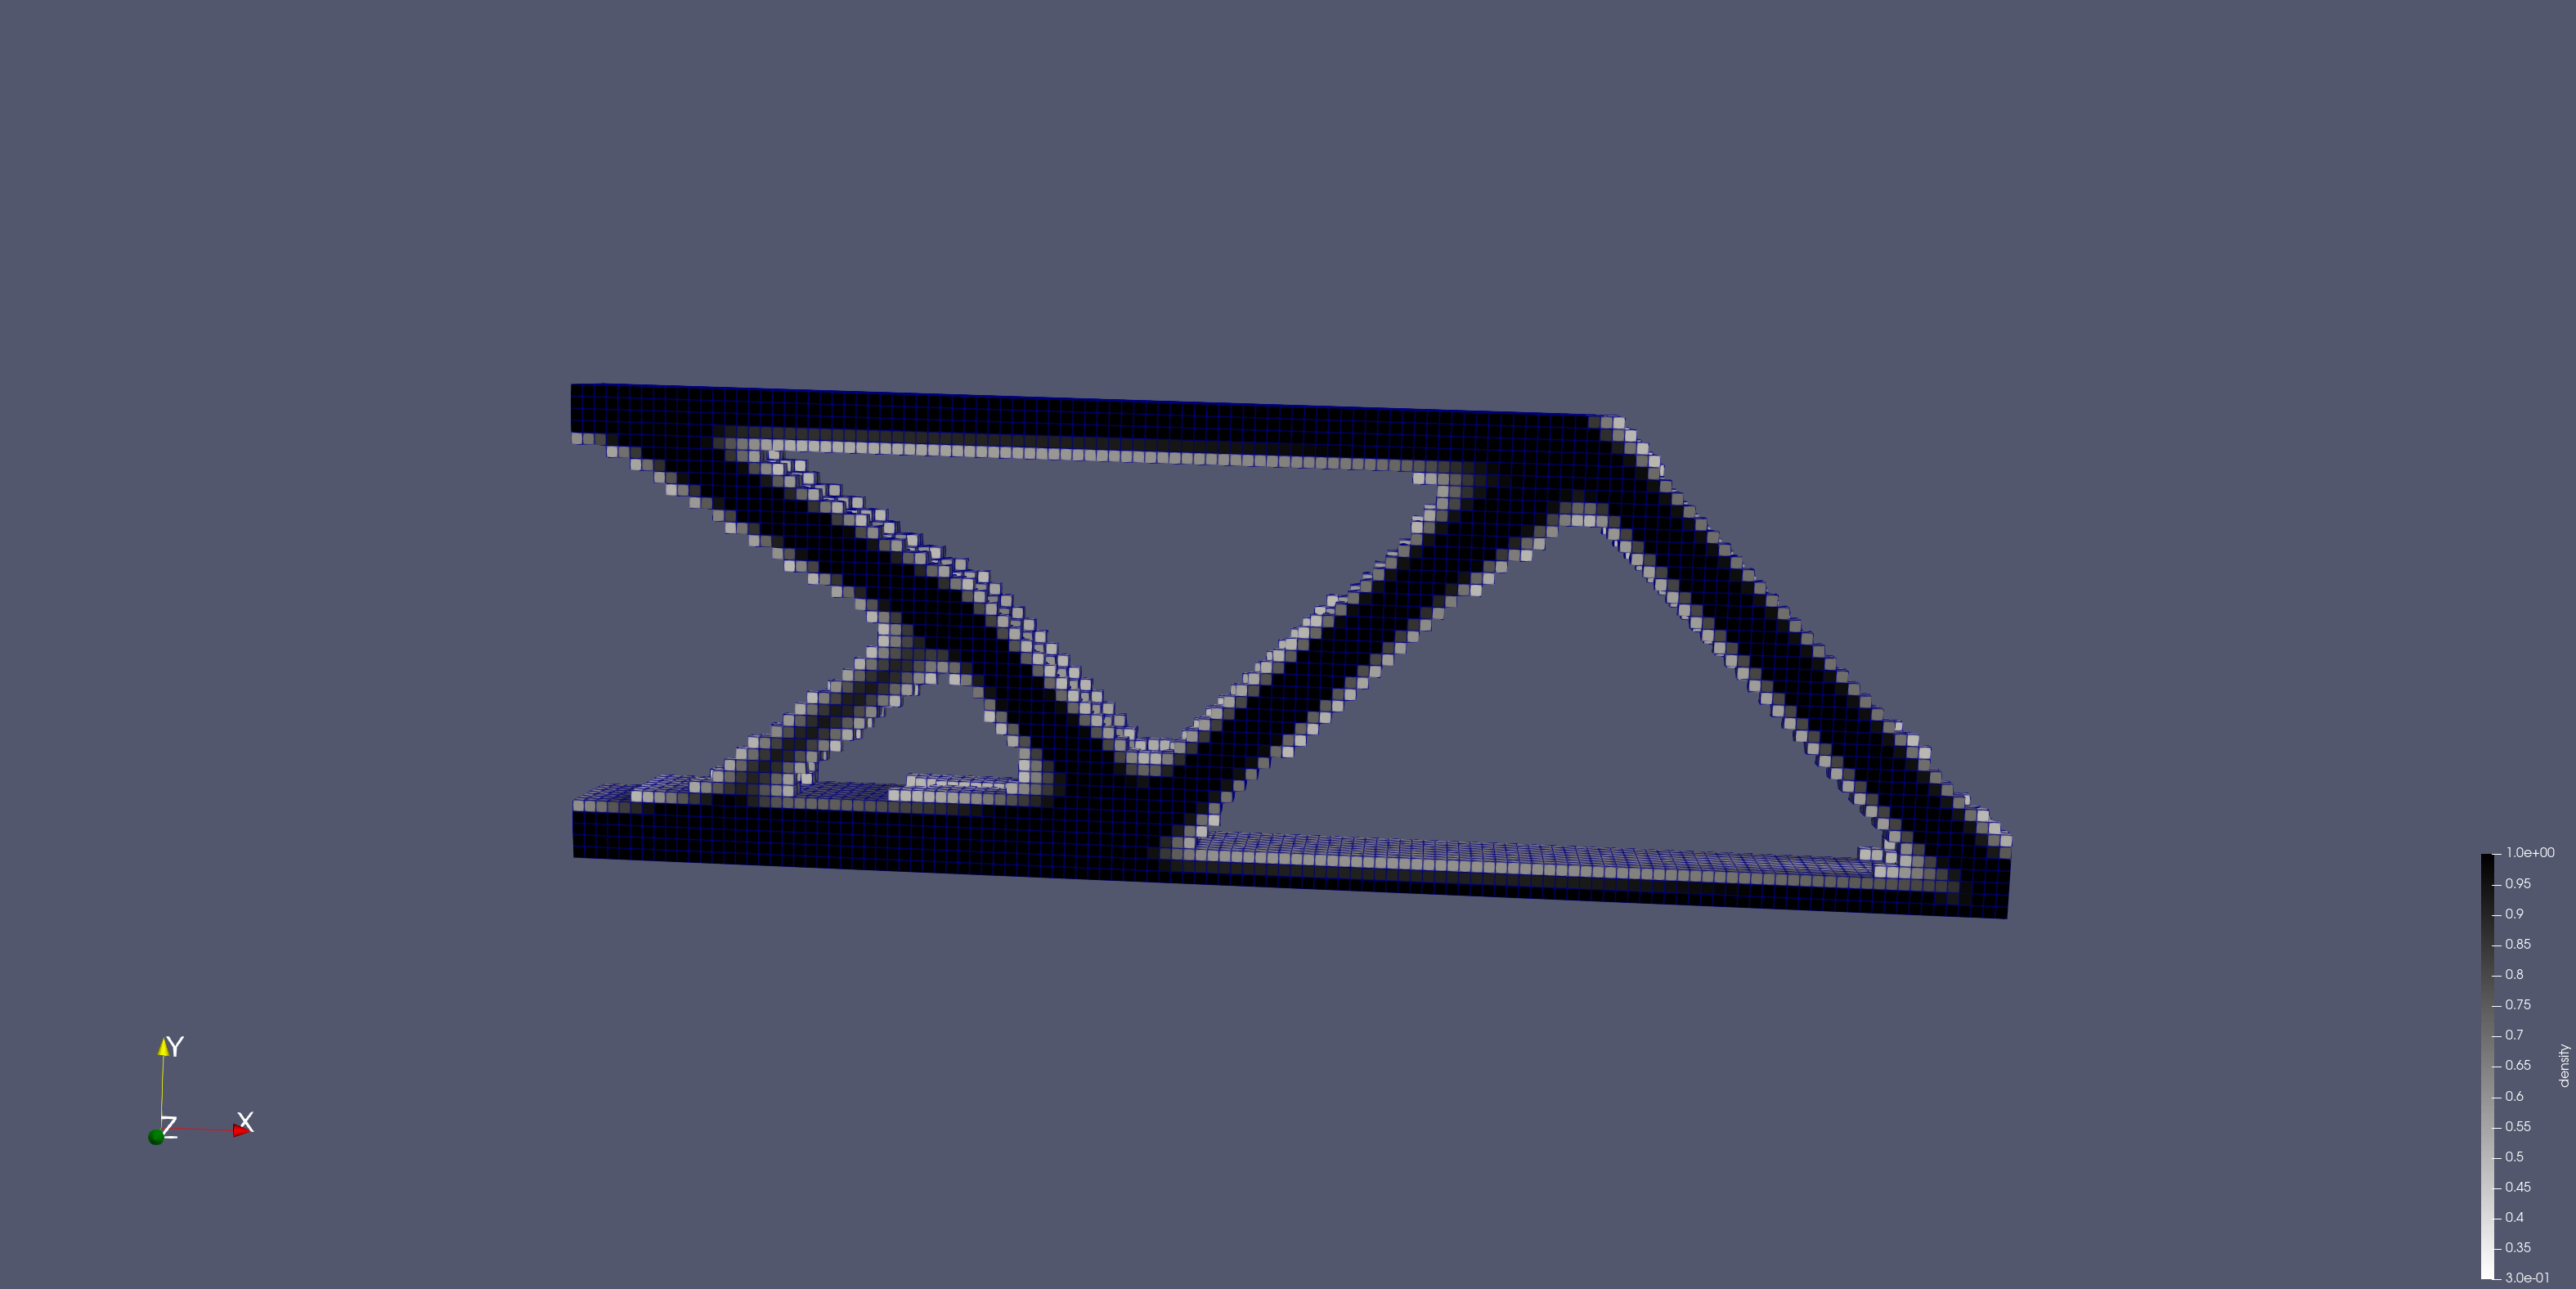
\includegraphics[width=0.5\textwidth]{figures/cantilever_3d_cpu.png}
		\label{fig:canti3d_cpu}
	}
	\subfloat[$c(\rho)=3494.2391,~v(\rho)=0.3000$]{
		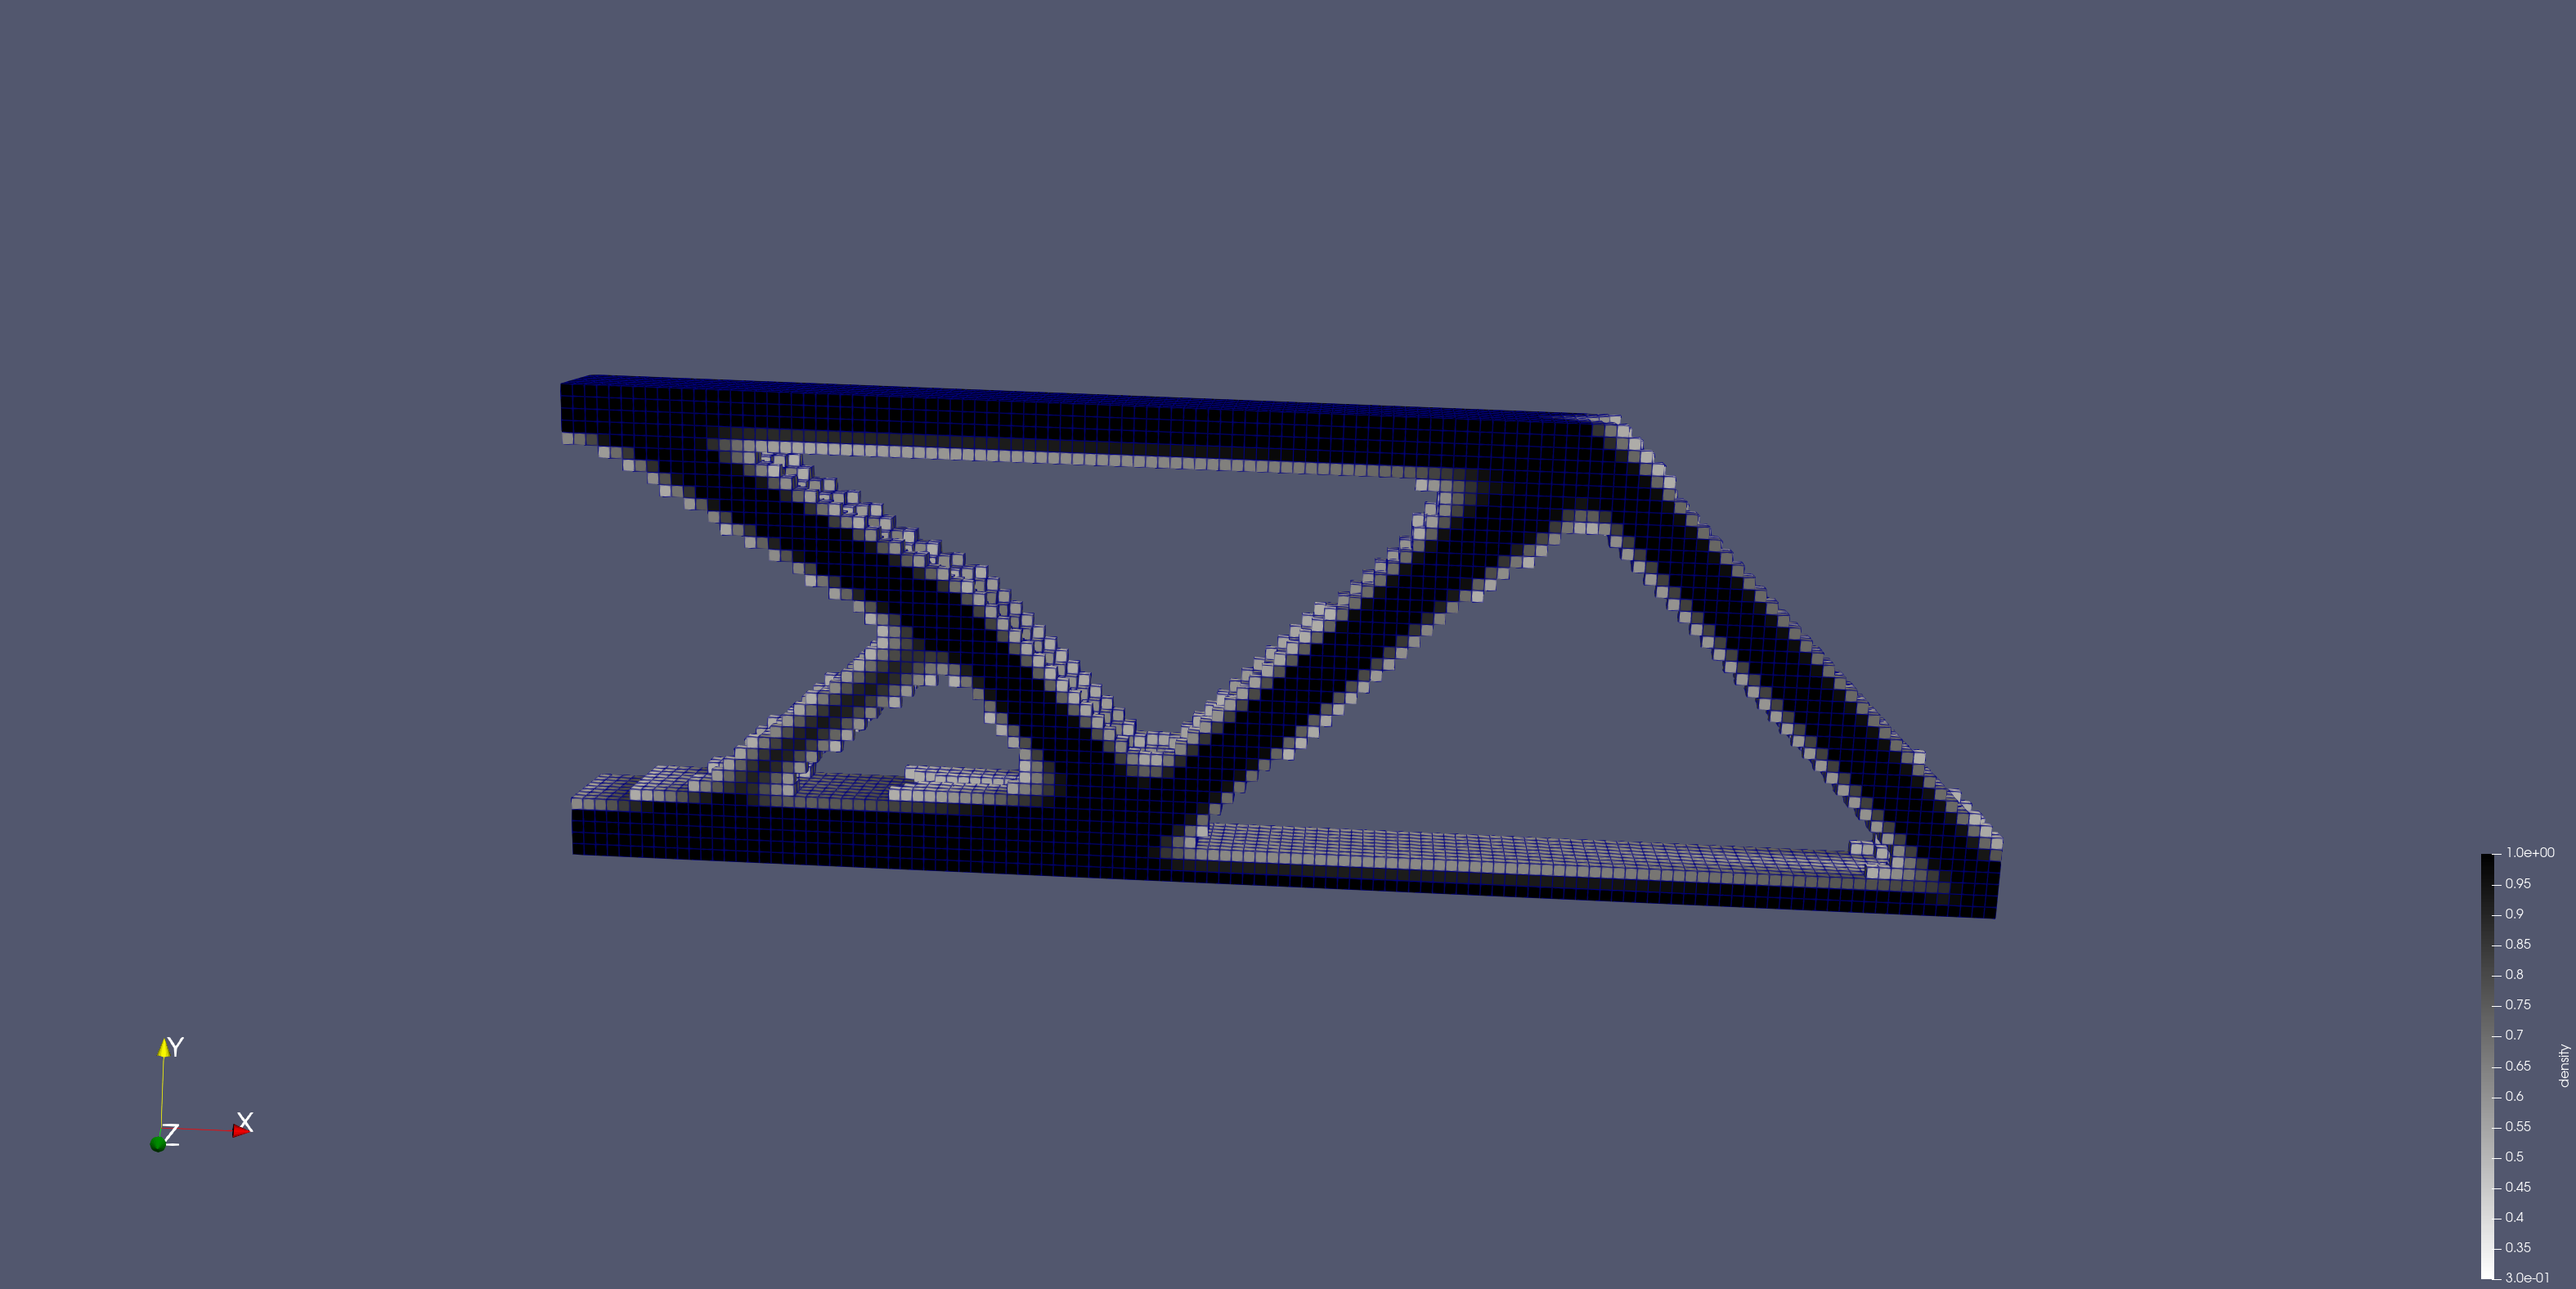
\includegraphics[width=0.5\textwidth]{figures/cantilever_3d_gpu.png}
		\label{fig:canti3d_gpu}
	}
	\caption{Optimized topologies of the 3D cantilever beam on CPU (left) and GPU (right), with elements of density $\rho > 0.3$ visualized.}
	\label{fig:canti3d_device_compare}
\end{figure}

As shown in Figure~\ref{fig:canti3d_device_compare}, the optimized topologies obtained using the CPU and GPU are highly similar. Although slight differences are observed in the final compliance ($c(\rho)$) and volume fraction ($v(\rho)$)—both within $1\%$---these discrepancies are attributed to minor variations in floating-point arithmetic precision and parallel implementation strategies across different hardware platforms. Nevertheless, in TO, such minor differences are negligible and do not affect the quality or performance of the final design.

Based on the consistency of the optimization results, we further compare the computational efficiency between the CPU and GPU. The detailed performance data are summarized in Table~\ref{tab:device_performance}.
\begin{table}[htbp]
	\centering
	\setlength{\tabcolsep}{4pt} % 减小列间距
	\caption{Performance comparison between CPU and GPU for the 3D cantilever beam optimization problem.}
	%	\small % 使用小字体
	\begin{tabular}{ccccc}
		\toprule
		\textbf{Computational Device} & \textbf{Iterations} & \textbf{Total Time (s)} & \textbf{1st Iter. Time (s)} & \textbf{Avg. Iter. Time (s)} \\
		\midrule
		CPU (PyTorch) & 155 & 3872.041 & 15.846 & 25.040 \\
		GPU (PyTorch) & 155 & 479.412 & 2.111 & 3.099 \\
		\bottomrule
	\end{tabular}
	\label{tab:device_performance}
\end{table}

As shown in Table~\ref{tab:device_performance}, GPU acceleration significantly reduces the total optimization time from \SI{3872.041}{s} on the CPU to \SI{479.412}{s} on the GPU, achieving an approximate speedup of $8.1$ times. The GPU outperforms the CPU in both the first iteration and subsequent iterations, clearly demonstrating its advantages in parallel computing.

When using the CG method, the first iteration time (CPU: \SI{15.846}{s}, GPU: \SI{2.111}{s}) is notably lower than the average subsequent iteration time (CPU: \SI{25.040}{s}, GPU: \SI{3.099}{s}). This behavior is due to the fact that, at the initial stage of optimization, the material density distribution is relatively uniform, resulting in a stiffness matrix with a low condition number, allowing the CG method to converge quickly. As the optimization progresses and the material distribution becomes more heterogeneous, the condition number of the matrix deteriorates, requiring more internal CG iterations for convergence, thus increasing the computational time per iteration.

\section{Conclusion}
This work presents SOPTX, a high-performance topology optimization (TO) framework based on FEALPy. A series of classical benchmark examples have been conducted to validate the effectiveness and practicality of SOPTX in solving TO problems. The development of SOPTX is entirely based on the open-source software FEALPy, without relying on any commercial software. This fully open-source nature not only lowers the technical barrier but also enables users to easily access, learn, and utilize the framework, making it particularly suitable for academic research and educational purposes.

The core innovations of SOPTX are reflected in the following three aspects:
\begin{enumerate} 
	\item \textbf{Modular Design Framework}: Through a loosely coupled architecture, SOPTX supports topology optimization problems in both two and three dimensions, as well as various mesh types (structured and unstructured). It provides a rich library of combinable components, enabling users to flexibly configure and extend the optimization workflow.
	\item \textbf{Cross-Platform Multi-Backend Support and Automatic Differentiation}: Numerical results show that GPU computations take only approximately $33\%$ of the CPU time. Leveraging AD, SOPTX enables the automatic computation of gradients for objective and constraint functions, simplifying sensitivity analysis, reducing development difficulty, and improving computational accuracy.
	\item \textbf{Fast Matrix Assembly Technique}: By optimizing the matrix assembly process, reducing redundant computations, and exploiting matrix sparsity, SOPTX significantly improves finite element matrix assembly efficiency. Benchmark results demonstrate that the average assembly time is reduced from \SI{0.838}{s} to \SI{0.273}{s}, corresponding to approximately $33\%$ of the original method.
\end{enumerate}

Through the example analyses presented in Sections~\ref{sec:exp_mbb_beam} to~\ref{sec:exp_multi_backend}, SOPTX demonstrates outstanding performance in model switching, filter method selection, optimization algorithm flexibility, three-dimensional extension, computational efficiency enhancement, application of automatic differentiation, and multi-backend switching, fully validating its technical advantages.

Although SOPTX currently focuses primarily on density-based TO, it holds promising potential for future development. Leveraging the capabilities of FEALPy in solving heat conduction and Navier–Stokes equations, SOPTX can be extended to optimize thermo-fluid-structure coupling problems, such as thermal protection system designs in aerospace applications or heat dissipation optimization in electronic devices. 

By integrating FEALPy's level set solver module, SOPTX can also support boundary-clear level set methods, enabling the generation of smooth boundaries suitable for precision manufacturing scenarios. In addition, the incorporation of FEALPy's adaptive mesh refinement techniques—particularly local mesh refinement near boundaries---could further enhance the solution accuracy for complex geometries and improve the geometric details of optimized structures. 

Moreover, SOPTX plans to support stress constraints and manufacturing constraints, especially targeting applications in 3D printing and additive manufacturing. Future extensions may include overhang angle control and support structure optimization, aiming to reduce the use of support materials, improve printing efficiency, and meet the high standards of lightweight design and manufacturability required in fields such as aerospace, automotive engineering, and biomedical engineering.

In summary, SOPTX significantly enhances research and development efficiency in the field of TO through its modular design, automatic differentiation capabilities, and multi-backend support. Its open-source nature further lowers the barrier to adoption. Compared to other implementations, SOPTX exhibits notable advantages in computational efficiency, flexibility, and ease of use, providing a solid foundation for both academic research and industrial applications. Looking ahead, SOPTX is expected to play a greater role in multiphysics optimization, lightweight structural design, and additive manufacturing, accelerating the widespread adoption and application of TO in industrial design and manufacturing.

%%%% Acknowledgments %%%%%%%%
\section*{Acknowledgments}
The first and fourth authors were supported by the National Natural Science
Foundation of China (NSFC) (Grant No. 12371410, 12261131501), and the
construction of innovative provinces in Hunan Province (Grant No. 2021GK1010).
The second author was supported by NSF DMS-2012465 and DMS-2309785. The third
author was supported by the National Natural Science Foundation of China (NSFC)
(Grant No. 12171300), and the Natural Science Foundation of Shanghai (Grant No.
21ZR1480500).

\appendix
\renewcommand{\thesection}{Appendix\,\Alph{section}}
\section{Cantilever2dData1}
\label{sec:code_canti_2d}
\begin{lstlisting}[language=python]
class Cantilever2dData1:
	def __init__(self, 
				xmin: float, xmax: float, 
				ymin: float, ymax: float,
				T: float = -1):
	self.xmin, self.xmax = xmin, xmax
	self.ymin, self.ymax = ymin, ymax
	self.T = T 
	self.eps = 1e-12
	
	def domain(self) -> list:
		box = [self.xmin, self.xmax, self.ymin, self.ymax]
		return box
	
	@cartesian
	def force(self, points: TensorLike) -> TensorLike:
		domain = self.domain()
		x = points[..., 0]
		y = points[..., 1]
		coord = (
			(bm.abs(x - domain[1]) < self.eps) & 
			(bm.abs(y - domain[2]) < self.eps)
			)
		kwargs = bm.context(points)
		val = bm.zeros(points.shape, **kwargs)
		val[coord, 1] = self.T
		return val
	
	@cartesian
	def dirichlet(self, points: TensorLike) -> TensorLike:
		kwargs = bm.context(points)
		return bm.zeros(points.shape, **kwargs)
	
	@cartesian
	def is_dirichlet_boundary_dof_x(self, points: TensorLike) -> TensorLike:
		domain = self.domain()
		x = points[..., 0]
		coord = bm.abs(x - domain[0]) < self.eps
		return coord
	
	@cartesian
	def is_dirichlet_boundary_dof_y(self, points: TensorLike) -> TensorLike:
		domain = self.domain()
		x = points[..., 0]
		coord = bm.abs(x - domain[0]) < self.eps
		return coord    
	
	def threshold(self) -> Tuple[Callable, Callable]:
		return (self.is_dirichlet_boundary_dof_x, 
				self.is_dirichlet_boundary_dof_y)
\end{lstlisting}

\section{MBBBeam2dData1}
\label{sec:code_mbb}
\begin{lstlisting}[language=python]
class MBBBeam2dData1:
def __init__(self, 
			xmin: float=0, xmax: float=60, 
			ymin: float=0, ymax: float=20,
			T: float = -1):
	self.xmin, self.xmax = xmin, xmax
	self.ymin, self.ymax = ymin, ymax
	self.T = T
	self.eps = 1e-12

def domain(self) -> list:
	box = [self.xmin, self.xmax, self.ymin, self.ymax]
	return box

@cartesian
def force(self, points: TensorLike) -> TensorLike:
	domain = self.domain()
	x = points[..., 0]
	y = points[..., 1]
	coord = ((bm.abs(x - domain[0]) < self.eps) & 
			 (bm.abs(y - domain[3]) < self.eps))
	kwargs = bm.context(points)
	val = bm.zeros(points.shape, **kwargs)
	val[coord, 1] = self.T
	return val

@cartesian
def dirichlet(self, points: TensorLike) -> TensorLike:
	kwargs = bm.context(points)
	return bm.zeros(points.shape, **kwargs)

@cartesian
def is_dirichlet_boundary_dof_x(self, points: TensorLike) -> TensorLike:
	domain = self.domain()
	x = points[..., 0]
	coord = bm.abs(x - domain[0]) < self.eps
	return coord

@cartesian
def is_dirichlet_boundary_dof_y(self, points: TensorLike) -> TensorLike:
	domain = self.domain()
	x = points[..., 0]
	y = points[..., 1]
	coord = ((bm.abs(x - domain[1]) < self.eps) &
			 (bm.abs(y - domain[0]) < self.eps))
	return coord

def threshold(self) -> Tuple[Callable, Callable]:
	return (self.is_dirichlet_boundary_dof_x, 
			self.is_dirichlet_boundary_dof_y)
\end{lstlisting}

\section{Cantilever3dData1}
\label{sec:code_canti_3d}
\begin{lstlisting}[language=python]
class Cantilever3dData1:
	def __init__(self,
				xmin: float=0, xmax: float=60, 
				ymin: float=0, ymax: float=20,
				zmin: float=0, zmax: float=4,
				T: float = -1):
		self.xmin, self.xmax = xmin, xmax
		self.ymin, self.ymax = ymin, ymax
		self.zmin, self.zmax = zmin, zmax
		self.T = T 
		self.eps = 1e-12
	
	def domain(self) -> list:
		box = [self.xmin, self.xmax, 
		self.ymin, self.ymax, 
		self.zmin, self.zmax]
		return box
	
	@cartesian
	def force(self, points: TensorLike) -> TensorLike:
		domain = self.domain()
		x = points[..., 0]
		y = points[..., 1]
		z = points[..., 2]
		coord = ((bm.abs(x - domain[1]) < self.eps) & 
				 (bm.abs(y - domain[2]) < self.eps))
		kwargs = bm.context(points)
		val = bm.zeros(points.shape, **kwargs)
		val[coord, 1] = self.T
		return val
	
	@cartesian
	def dirichlet(self, points: TensorLike) -> TensorLike:
		kwargs = bm.context(points)
		return bm.zeros(points.shape, **kwargs)
	
	@cartesian
	def is_dirichlet_boundary_dof_x(self, points: TensorLike) -> TensorLike:
		domain = self.domain()
		x = points[..., 0]
		coord = bm.abs(x - domain[0]) < self.eps
		return coord
	
	@cartesian
	def is_dirichlet_boundary_dof_y(self, points: TensorLike) -> TensorLike:
		domain = self.domain()
		x = points[..., 0]
		coord = bm.abs(x - domain[0]) < self.eps
		return coord
	
	@cartesian
	def is_dirichlet_boundary_dof_z(self, points: TensorLike) -> TensorLike:
		domain = self.domain()
		x = points[..., 0]
		coord = bm.abs(x - domain[0]) < self.eps
		return coord
	
	def threshold(self) -> Tuple[Callable, Callable]:
		return (self.is_dirichlet_boundary_dof_x, 
				self.is_dirichlet_boundary_dof_y,
				self.is_dirichlet_boundary_dof_z)
\end{lstlisting}

\section{Automatic Differentiation}
\label{sec:ad_compliance}
\begin{lstlisting}[language=python]
def _compute_gradient_auto(self, rho: TensorLike, u: Optional[TensorLike] = None) -> TensorLike:
	if u is None:
		u = self._update_u(rho)
	
	ke0 = self.solver.get_base_local_stiffness_matrix()
	cell2dof = self.solver.tensor_space.cell_to_dof()
	ue = u[cell2dof] 
	
	def compliance_contribution(rho_i: float, ue_i: TensorLike, ke0_i: TensorLike) -> float:
		E = self.materials.calculate_elastic_modulus(rho_i)
		c_i = -E * bm.einsum('i, ij, j', ue_i, ke0_i, ue_i)
		return c_i
	
	vmap_grad = bm.vmap(lambda r, u, k:bm.jacrev(lambda x: 
		compliance_contribution(x, u, k))(r))
	dc = vmap_grad(rho, ue, ke0)
	return dc
\end{lstlisting}


%%%% Bibliography  %%%%%%%%%%
\bibliographystyle{abbrv}
\bibliography{paper}


%\begin{thebibliography}{99}
%\bibitem{Berger}M. J. Berger and P. Collela, Local adaptive mesh refinement
%for shock hydrodynamics,
%J. Comput. Phys., 82 (1989), 62-84.
%\bibitem{deBoor}C. de Boor,  Good Approximation By Splines With Variable Knots II, in Springer Lecture
% Notes Series 363, Springer-Verlag, Berlin, 1973.
%\bibitem{TanTZ} Z. J. Tan, T. Tang and Z. R. Zhang, A simple moving mesh method for one- and
%two-dimensional phase-field equations, J. Comput. Appl. Math., to appear.
%\bibitem{Toro}E. F. Toro, Riemann Solvers and Numerical Methods for Fluid Dynamics,
%Springer-Verlag Berlin Heidelbert, 1999.
%\end{thebibliography}

\end{document}
